\documentclass[UTF8,oneside]{ctexbook}
\usepackage{amsmath,amssymb,tikz,xcolor,array}
\usepackage{geometry}
\geometry{a4paper,hmargin=2.5cm,vmargin=2cm}
\usetikzlibrary{math}
\usetikzlibrary{calc}
\newcommand\standardstate{{\circ\kern-0.495em-}}%我大抵是疯了,一定要它左右出头
\NewDocumentCommand\ch{m}{\(\mathrm{#1}\)}



\newcommand{\bookname}{大气化学}
\newcommand{\uira}{https://github.com/ZhangtongCN}
\newcommand{\uirb}{https://github.com/Clignniis}
\usepackage[toc]{multitoc}%双栏目录
%颜色设置
\usepackage{xcolor}
\definecolor{nuist}{RGB}{0, 103, 156}%南信大蓝
\definecolor{sky}{RGB}{101, 170, 221}%天空蓝
\definecolor{tech}{RGB}{38, 96, 173}%科技蓝
\definecolor{gold}{RGB}{201, 160, 99}%高贵金
%引用
\usepackage[colorlinks]{hyperref}
%设置页眉页脚

%章节设置
\ctexset{
    chapter={pagestyle=fancy},%使得章节页页眉页脚格式一致
}
\geometry{a4paper,top=2.5cm,bottom=2.5cm}
\setcounter{tocdepth}{1}
\linespread{1.3}\selectfont

%页眉页脚
\usepackage{fancyhdr}
\pagestyle{fancy}
\renewcommand{\sectionmark}[1]{\markright{\thesection\ #1}}
\fancyhf{}
\fancyhead[L]{\href{\uira}{\textcolor{tech}{\bookname}}}
\fancyhead[R]{\href{\uira}{\textcolor{tech}{笔记整理与汇总}}}
\fancyfoot[C]{\href{\uirb}{\textcolor{tech}{\thepage}}}
\renewcommand{\headrulewidth}{0pt}
\setlength{\headheight}{27pt}



\begin{document}

\frontmatter

\begin{titlepage}
    \begin{tikzpicture}[remember picture, overlay]
        \node at ([shift={(0,1)}]current page.center){
            \begin{tikzpicture}[scale=0.7]
            \path[fill=sky] (0:0)--++(90:2)--++(30:6)--++(150:6)--++(210:6)--++(330:6)--++(90:1)--++(150:4)--++(30:4)--++(330:4)--++(210:4)--++(270:3)--++(150:1)--++(210:3)--++(270:1)--++(30:5)--++(330:3)--++(270:1)--++(210:4)--++(150:4)--++(210:1)--++(330:5)--++(30:5)--cycle;
            \path[fill=cyan!50] (0:0)--++(270:1)--++(210:3)--++(150:1)--++(90:5)--++(150:1)--++(270:6)--++(30:6)--++(90:1)--++(30:4)--++(270:6)--++(210:5)--++(270:1)--++(30:6)--++(90:8)--++(210:6)--cycle;
            \path[fill=cyan!50] (90:6)--++(90:1)--++(210:4)--++(330:1)--++(30:3)--++(90:1);
            \path[fill=nuist] (0:0)--++(270:1)--++(330:3)--++(30:1)--++(90:5)--++(30:1)--++(270:6)--++(150:6)--++(90:1)--++(150:4)--++(270:6)--++(330:5)--++(270:1)--++(150:6)--++(90:8)--++(330:6)--cycle;
            \path[fill=nuist] (90:6)--++(90:1)--++(330:4)--++(210:1)--++(150:3)--++(90:1);
            \end{tikzpicture}
        };
        \node at ([shift={(0,8)}]current page.center){\href{\uirb}{\fontsize{72}{0}\heiti\textcolor{gold}{\bookname}}};
        \node at ([shift={(0,-5)}]current page.center){\Huge\heiti\href{\uira}{\textcolor{nuist}{Tong Zhang}}\quad\href{\uirb}{\textcolor{nuist}{Cls}}};
        \node[anchor= south] at ([shift={(0,6)}]current page.south){\href{\uirb}{\fontsize{48}{0}\heiti \textcolor{tech}{笔记整理与汇总}}};
    \end{tikzpicture}
\end{titlepage}

\chapter*{版权声明}

本《\bookname{} 笔记整理与汇总精编版》一册电子版遵循有限的知识共享许可协议。本书授权包含署名-非商业性使用-相同方式共享(CC BY-NC-SA)。即您被允许在授权范围内对该电子书进行转载、节选、二次创作,但不得用于任何商业目的,且使用时须署原作名,且必须采用与本创作相同的协议(CC BY-NC-SA)进行授权。限于编者水平,本书难免有疏漏错误,敬请读者批评指正。

由于更新安排调整,本文档未经过完整核对,可能存在较多错误。
\begin{tikzpicture}[remember picture, overlay]
    \node [opacity=1] at ([shift={(-4,4)}]current page.south east){
        \begin{tikzpicture}[scale=0.5]
            \foreach \a in {1,0.8,...,0.2} {%
                \draw (-\a,1) circle [radius=\a];
                \draw (-2+\a,-1) circle [radius=\a];
                \draw (2-\a,-1) circle [radius=\a];
            }
        \end{tikzpicture}
    };
\end{tikzpicture}

\tableofcontents

\mainmatter

\chapter{绪论}
\section{课程简介}
\subsection{简介}
\begin{description}
    \item[简介] 研究对环境有重要影响的大气组分的大气化学行为的学科,是环境科学、大气科学的一个分支。实质上研究大气中污染物的问题。
    \item[组分] 不是平时意义上理解的氮气、氧气、氩气,而是浓度非常低的物质,如臭氧、氮氧化物、硫化物等
    \item[化学行为] 大气化学行为指大气中化学物质通过化学反应、迁移转化、浓度变化、生成消耗及循环过程,与大气组分、环境及气候系统相互作用并影响其动态平衡的物理化学活动。
    \item[研究范畴] 我们研究的大气特指地球大气,不研究其他行星大气。不止研究大气,涉及各圈层的研究。
    \item[总体角度] 来源角度+天气角度
\end{description}
\subsection{大气化学历史}
\begin{description}
    \item[总结] 约70年,蓬勃发展中  局地→区域→全球  高浓度→微量→痕量
    \item[1950年代]
    \begin{description}
        \item[洛杉矶光化学烟雾] (主要由\ch{O_3},VOCs,\(\mathrm{NO}_x\)组成)。 降水化学,关注气溶胶
        \begin{description}
            \item[污染源] 机动车尾气排放大量\(\mathrm{NO}_x\)和VOCs(如烯烃、芳香烃)。
            \item[光化学反应] 氮氧化物在紫外线下光解,VOCs与OH自由基反应生成过氧自由基,减少\ch{O_3}消耗,导致\ch{O_3}累积,并生成二次污染物。
            \item[气象条件] 高温、低湿度、强日照及逆温层阻碍污染物扩散。
        \end{description}
        \item[伦敦烟雾](\ch{SO_2})火电厂燃煤释放二氧化硫,快速氧化形成硫酸盐气溶胶
        \begin{description}
            \item[污染源] 燃煤释放、颗粒物烟尘及。
            \item[气象条件] 低温、高湿度、静稳天气及逆温层导致污染物近地面聚集。
        \end{description}
    \end{description}
    \item[1960年代] 城市大气污染与核扩散,光化学烟雾,\ch{CO_2}定量研究,酸雨问题
    \item[1970年代] 平流层臭氧(南极臭氧空洞),输送,关注自由基,元素生物地球化学循环
    \item[1980年代] 对流层臭氧化学,温室气体及其气候效应,云雾化学,有害金属(如汞砷)、非金属气体循环等
    \item[1990年代后] 大气化学组分变化,酸雨,气溶胶/霾化学,大气污染与气候等等。氧化性大气:氧化性强的自由基,影响大气物质寿命
    \item[我国历史] 我国大气化学约起于1970年代(1974年兰州光化学烟雾事件,石油化工工业+强光+山谷不易扩散)
\end{description}
\subsection{研究方法}
\begin{description}
    \item[主要方法] 现场实测、实验室研究、数值模拟  三者相互联系
\end{description}

例如,某城市发生污染。首先需要观测取样,了解发生污染类型、浓度变化、联系探讨;随后用已有理论研究解释,如果无法解释,可以提出新的假设和理论,并在实验室中检验、重现、探讨反映条件、过程等,提出新机制;最后在模式中加入相关化学反应,对比真实情况与实际情况,验证新机制,得到相关结论,提高预测预报准确度,对来源做解析、情景分析、评估对策有效性等。

野外观测还能为后者提供基础数据,是联系实际和理论的桥梁。实验室做机理研究,模式做实际应用(有时效性的要求)。

\begin{description}
    \item[研究目标] 人类活动排放大量污染物,并引起局部严重污染及至全球气候变化等一系列问题。为解决此类空气污染问题,我们需要深刻理解排放物如何影响大气成分以及其化学行为与污染物与天气气候的相互作用。
\end{description}
\section{基础知识}
\subsection{大气演化}
\begin{description}
    \item[大气] 大气层厚度一般在100km,大气化学关注对流层0-20km。
    \item[大气组分] 主要是\ch{N_2}、\ch{O_2},次要有\ch{H_2O}、\ch{CO_2},惰性气体Ar、He等,其他气体有\ch{CH_4}、\ch{N_2}O等。
    \item[三代大气] 
    \begin{description}
        \item[一代] 原始大气,由星云气体组成,主要为氢气、氦气(逸散太空)【还原性大气】。
        \item[二代] 次生大气,由第一代大气减去蒸腾气体,加上火山喷发气体,加上来自彗星与其他天体的气体化学反应,海洋平衡,岩石风化。多为二氧化碳、甲烷、氨、水汽。
        \item[三代] 现代大气,由生命出现与氧气增加为特点(氧氮充分)【氧化性大气】。开始主要由\ch{N_2}组成,后期氧气增多。
    \end{description}
    \item[次生大气] 喷发物:85\%水汽、10\%二氧化碳、少量氮、硫化氢、氨气、甲烷。有氧原子,但没有氧气。
    \item[具体组分] 氧(<1\%,光致水解而成)、硫(硫化氢)、碳(二氧化碳与大量CO,200-1000倍于当下,目前溶解于海洋)、氮(与现代相似)
    \item[三代演变步骤] 生命创建→产氧菌类形成→植物覆盖地球
    \begin{description}
        \item[1生命创建] 有机汤试验、深海热泉
        \item[2氰基菌类] 最早产氧菌类,制造吸氧生物所需氧气,水生与光合\(\mathrm{H_2O}+\mathrm{CO}_2=\)糖+氧
        \item[3植物与氧气增加] 单细胞植物出现在27亿年前,与氧气快速上升同步,大气随后发展受生命驱动。大气演化含量峰值曾达35\%(3亿年前),后降到11\%(2.5亿年前)有研究指出目前氧气含量以每年4ppm速度减少
    \end{description}
\end{description}
\subsection{大气分层}
\begin{description}
    \item[均质划分] 90km以下,空气平均分子量为28.966,不随高度变化;90km以上,随高度递减。
    \item[电离分层] 
\begin{description}
    \item[中性层] <60km,地壳和大气中的放射性物质主要对低层大气的电离起作用,作用较弱
    \item[电离层] >60km,宇宙线和太阳紫外线辐射对高层大气起作用,作用较强
\end{description}
    \item[温度分层]
\begin{description}
    \item[对流层] 质量占比>80\%,几乎所有水汽、云和降水,非常强垂直混合,温度随高度递减。赤道15-20km,极地8-14km,南京11-17km
    \item[平流层] 较弱的垂直混合,温度随高度递增,含有臭氧层(50km)\\
    若有污染物进入,会快速扩散,长期存在(但有光解反应,产生自由基,破坏臭氧)
    \item[中间层] 温度随高度递减,较强的垂直运动(85km)
    \item[热层] 温度随高度递增,高度电离,带电粒子运动受地磁场作用(磁层550km)
    \item[外层] 温度增加不显著,大气成分散逸至星际空间
\end{description}
    \item[边界层] 1-2km,上方一般存在逆温层。边界层高度由于太阳加热白天增加,且夏季偏高。如果边界层很低,污染物浓度相应升高;反之可推。
\end{description}
\subsection{大气压强}
\subsubsection{压强基本内容}
\begin{description}
    \item[定义] 大气压是作用在单位面积上的大气压力,在数值上为单位面积上延伸到大气上界的垂直空气柱的重力
    \item[基本表达] \(P_\mathrm{A}=\rho gh\)
    \item[基本数值] \(\rho_\text{水银}=13.6\mathrm{g\cdot cm^{-3}}\quad h=760\mathrm{mm}\)\\
    海平面平均气压为\(1013\mathrm{hPa}\sim10^5\mathrm{Pa}\)。全球地表平均气压为985.5hPa,相当于1.5km高度的大气压
    \item[延伸单位]
    \begin{enumerate}
        \item 帕斯卡 1MPa=1000kPa
        \item 巴 1kPa=1mbar
        \item 托尔
        \item 工程公斤力
        \item Psi 磅/平方英寸
        \item 标准大气压 1atm=1013hPa
    \end{enumerate}
    \item[状态方程]\(pV=nRT,p=\rho RT,R=8.314\mathrm{J\cdot mol^{-1}\cdot K^{-1}}\)
    \item[假设] 
    \begin{enumerate}
        \item 气体分子间无相互作用力
        \item 气体分子不占据体积
    \end{enumerate}
\end{description}
\subsubsection{大气压随高度的变化}
\begin{figure}[htbp]
    \centering
    \begin{tikzpicture}[>=latex]
        \fill[gray](0,0) rectangle (5,1);
        \draw[<->](0,-0.2)--node[below]{单位面积}(5,-0.2);
        \node[right] at (5,0){\(P(z)\)};
        \node[right] at (5,1){\(P(z+\mathrm{d}z)\)};
    \end{tikzpicture}
\end{figure}
\begin{description}
    \item[推导] 考虑一个单位面积空气团:\(P(z)=P(z+\mathrm{d}z)+\rho_ag\,\mathrm{d}z\Rightarrow\frac{\mathrm{d}P}{\mathrm{d}z}=-\rho_ag\)又有\(\rho_a=\frac{PM_a}{RT}\Rightarrow\frac{\mathrm{d}P}{P}=-\frac{M_ag}{RT}\,\mathrm{d}z\)其中\(M_a=28.97\mathrm{g}\cdot\mathrm{mol}^{-1}\)是空气的平均摩尔质量
    \item[公式] 假设温度不变,最终可得到:\(P(z)=P(0)\mathrm{e}^{-z/H}\)类似地,\(\rho(z)=\rho(0)\mathrm{e}^{-z/H}\)
    \item[大气标高] \(H=\frac{PT}{M_ag}\approx7.4\mathrm{km}\)(对流层均温为253K)压强为地表的1/e
    \item[测高公式] \(Z_2-Z_1=\frac{R_d\overline{T}_v}{g_0}\ln\left(\frac{p_1}{p_2}\right)\)
    \item[大气总质量] 总质量\(=4\pi R^2_e\rho_0\int_0^\infty\mathrm{e}^{-z/H}\,\mathrm{d}z=4\pi R^2_e\rho_0H\approx4.7\times10^{18}\mathrm{kg}\)(\(R_e\approx6400\mathrm{km},H\approx7.4\mathrm{km},\rho\approx1.23\mathrm{kg\cdot m^{-3}}\))考虑全球表面平均气压,进一步推导精确值:\(5.1480\times10^{18}\mathrm{kg}\)若不包括水汽,只计算干空气质量\(=5.1352\times10^{18}\mathrm{kg}\)
    \item[大气摩尔数] 总摩尔数:\(1.62\times10^{20}\mathrm{mol}\)总分子数:\(1.0\times10^{44}\mathrm{mol}\)
\end{description}
\subsection{大气组分单位}
\subsubsection{混合比}
\begin{description}
    \item[定义] Mixing ratio 某种物质在空气团中占的摩尔数的比值,主要对气态污染物使用\(\xi_i=\frac{c_i}{c_\mathrm{total}}=\frac{p_i/RT}{p/RT}=\frac{p_i}{p}\)实质为分压
    \item[说明]
    \begin{enumerate}
        \item 若包括水汽的话,混合比会有几个百分点的而变化,一般混合比定义是针对干空气而言的。
        \item 一般情况下,针对气体ppm是指体积比而非质量比;但若描述溶液中组分,一般指质量比。
    \end{enumerate}
    \item[常用单位]
    \begin{enumerate}
        \item ppm	意为parts per millon,\(10^{-6}\mu\)mol/mol
        \item ppb 	意为parts per billon,\(10^{-9}\)nmol/mol
        \item ppt 	意为parts per trillon,\(10^{-12}\)pmol/mol
        \item 有时候会添加一个(对体积):ppmv意为parts per millon by volume
        \item 有时候会添加一个(对质量):ppmm意为parts per millon by mass
    \end{enumerate}
    除此之外,还有很多体积混合比很低的痕量气体(),在大气化学反应中作用非常重要
\end{description}
\begin{table}[htbp]
    \centering
    \caption{一般数据}
    \begin{tabular}{|c|c|}
        \hline
        \ch{N_2} & 0.78\\
        \hline
        \ch{O_2} & 0.21\\
        \hline
        Ar & 0.0093\\
        \hline
        \ch{CO_2} & \(365\times10^{-6}\)\\
        \hline
        \ch{CH_4} & \(1.7\times10^{-6}\)\\
        \hline
        \ch{N_2O} & \(320\times10^{-9}\)\\
        \hline
    \end{tabular}
\end{table}
\subsubsection{水汽表达}
\begin{description}
    \item[体积混合比] 位于ppm量级mol/mol
    \item[质量混合比] 每千克干空气中水汽质量g/kg
    \item[比湿] 每千克空气中水汽质量g/kg
    \item[质量浓度] 单位体积内有多少克水汽\(\mathrm{g/m^3}\)
    \item[相对湿度] RH水蒸气分压与该温度下水蒸气饱和蒸汽压的比值
    \item[水汽分布] 水汽在地球表面混合比为百分之几,而在平流层则只有几个ppm(尤其是赤道上空)。这是因为温度骤降,大部分水汽结冰而被除去。
\end{description}
\subsubsection{排放量}
\begin{description}
    \item[定义] 某种物质向大气中的排放量一般以每年为单位表示
    \item[单位] Tg/year(\(1\mathrm{Tg}=10^{12}\mathrm{g}\))描述\ch{CO_2}排放常用Gigatons(\(1\mathrm{Gt}=10^{15}\mathrm{g}\))
\end{description}
\subsubsection{数浓度}
\begin{description}
    \item[气体] 分子个数/\(\mathrm{cm}^3\)常用于表示比还要低的浓度水平
    \item[颗粒物] 粒子个数/\(\mathrm{cm}^3\)
\end{description}
\subsection{单位转换}
\subsubsection{\(\mathrm{ppm}\Leftrightarrow\mu\mathrm{g/m^3}\)}
\begin{description}
    \item[一般情况] 某些时候,气体的浓度以混合比如ppb给出,颗粒物浓度以\(\mu\mathrm{g/m^3}\)给出,需要进行转换以便于对比
    \item[推导] 某物质浓度为\(m_i\),以\(\,mu\mathrm{g/m^3}\)表示,则该物质的摩尔浓度为:\(c_i=\frac{10^{-6}m_i}{M_i}\)其中\(M_i\)摩尔质量g/mol根据理想气体方程\(c=p/RT\)转换计算:\(ppm=\frac{8.314T}{pM_i}\times\text{concentration of }i\text{ in }\mu\mathrm{g/m^3}\)
    \item[典例] \(p=1\)atm和\(T=298\)K下\ch{O_3}混合比为120ppb,相当于多少\(\mu\mathrm{g/m^3}\)?
    \item[推导] 臭氧摩尔质量为48,混合比120ppb,即\(120\times10^{-9}\)mol/mol。\\
    则1mol大气中有质量\(120\times10^{-9}\times48\)g的臭氧。\\
    1mol大气有\(pv=nRT\),则\(v=\frac{nRT}{p}=\frac{1\times8.31\times298}{1.013\times10^5}=0.024446\)。\\
    故有1立方米大气中臭氧\(\frac{120\times10^{-9}\times48}{0.024446}=0.000235621\),则有\(235.621\mu\mathrm{g/m^3}\)
    \item[公式] \(\mu\mathrm{g/m^3}=\frac{pM_i}{8.314T}\times\text{Mixing ratio in ppm}=\frac{1.013\times10^5\times48}{8.314\times298}\times0.12=235.6\mu\mathrm{g/m^3}\)
\end{description}
\chapter{大气成分和排放源}
\section{大气污染物的主要来源}
\subsection{大气污染物的直接排放源(一次来源)}
\begin{description}
    \item[人为源]
    \begin{description}
        \item[化石燃料燃烧] 汽车尾气、电厂 (煤、汽油/柴油、天然气)
        \item[生物质燃烧] 烧柴火、秸秆焚烧等全球约一半人采用仍使用该方法
        \item[固废焚烧] 垃圾焚烧
        \item[工业] 化工、电子、家具制造、医药等
        \item[农业] 施肥、农药、甲烷释放、畜牧业等
        \item[扬尘] 建筑、交通
        \item[其他源] 油锅炒饭、吸烟、餐饮、干洗、化妆品挥发性有机物等
    \end{description}
    \item[天然源]
    \begin{description}
        \item[沙尘] 风吹尘、沙尘暴、土壤悬浮尘
        \item[海浪飞沫] 硫酸盐气溶胶、钠盐等 【全球最多】
        \item[野火] 生物质燃烧,草原、森林大火
        \item[火山喷发] 周期长、进入平流层,25km有硫酸盐层
        \item[生物(动植物)排放] 挥发性有机物
        \item[海洋浮游生物排放]
    \end{description}
\end{description}
\subsection{大气污染的生成(二次来源)}
\begin{description}
    \item[定义] 排放源直接排放到大气中的,直接排放的污染物称为一次污染物。而进入大气的某些一次污染物,受环境中物理的、化学的或生物的因素作用,转化生成的大气污染物则为二次污染物。
    \item[一次举例] 气溶胶(花粉、粉尘、黑炭)
    \item[二次举例] 臭氧(、光化学反应)、气溶胶(硫酸盐、铵盐、二次有机气溶胶)
\end{description}
\subsection{大气污染的类型(本节未教授)}
\begin{description}
    \item[典型类型] 一次污染(煤烟型)、二次污染(光化学烟雾型)
\end{description}
\subsubsection{复合污染}
\begin{description}
    \item[定义] 是指大气中由多种来源的多种污染物在一定的大气条件下(如温度、湿度、阳光等)发生多种界面间的相互作用彼此耦合构成的复杂大气污染体系。
    \item[复合含义]
    \begin{enumerate}
        \item 煤烟型污染与机动车尾气污染及其他污染相叠加
        \item 大气中均相反应和多相反应相耦合
        \item 局地与区域污染相互影响
    \end{enumerate}
    \item[结果] 二次污染物,尤其是颗粒物细粒子大量增加。后者是复合污染中具有综合信息的污染物,它可以来自于燃煤、机动车排放、生产和生活过程以及大气化学反应过程等。高浓度细粒子,能见度下降;大气氧化性增强,二次污染严重;一定气象条件下,呈区域性
\end{description}
\subsection{大气污染物来源分析技术}
\begin{description}
    \item[概述] 对污染物来源的研究是大气化学研究的一项基础工作,已发展了从传统的扩散模式到现在技术已经比较成熟的受体模式等方法,反向轨迹法是近年来正在探索的新方法。城市和区域尺度的来源研究通常采用的方法包括:源清单、扩散模型、受体模型
\end{description}
\subsubsection{源清单/排放清单}
\begin{description}
    \item[概念] 基于污染源的排放因子和源调查的一个基本来源研究方法
    \item[方法] 通过测定各种污染源的排放因子和调查统计不同污染源的排放活动数据来估算污染物的总排放量和确定不同源的贡献率
    \item[注意] 排放因子和源调查法概念上很简单易懂,但实际应用中有代表性的排放因子和外推的统计量都不易获得,因此这种“自下而上”的方法存在很大的不确定性。
\end{description}
\subsubsection{扩散模式/受体模式}
\begin{description}
    \item[扩散模式] 按照模式理论的发展途径可分为统计理论模式、K理论模式和相似理论模式\\
    按模拟的时间尺度可分为短期平均和长期平均浓度模式;\\
    按污染源的形态又可分为点源、线源、面源、体源、多源或复合源模式;\\
    从应用角度出发,实际工作中使用的大气扩散模式多属高斯模式及高斯模式的变型。\\
    美国、英国等国家已建立了比较完善的大气扩散模式系统,考虑了建筑物动力尾流效应、污染物衰变、重力沉降和干沉降以及特殊气象条件和不平坦地形等多种复杂因素,可以应用于模拟工业区、道路和城市乃至区域等复杂环境下大气污染物的浓度分布及源排放对环境的影响。比较有代表性的扩散模式主要有美国环保局推荐的复合工业源大气扩散模型(ISC)和非稳态烟团扩散模式(CALPUFF)等。
    \item[受体模式] 受体模式主要用于大气污染物的来源解析研究。\\
    在污染物从源到受体质量守恒且呈线性关系的假设下,受体模式通过分析受体点污染物的化学和物理特征来推断污染物的主要来源并估算各类源的贡献率。\\
    受体模式不依赖于气象资料和污染源清单,主要基于污染源排放特征、源排放化学成分谱和受体大气的物理化学特征,因此是一种典型的基于环境浓度的“自上而下”来源解析方法,能有效确定影响受体大气的主要污染源,避免了重要污染源的遗漏。\\
    最具代表性的受体模式是化学质量平衡(CMB)模式和正交矩阵因子分析(PMF)
\end{description}
\section{大气污染物的汇机制}
\begin{description}
    \item[概述] 各种大气污染物由源排放进入大气,在源附近浓度较高,随着与越来越多的空气混合而浓度逐渐被稀释。这个稀释过程可以被一系列的“汇机制” 加速,这些过程被称为污染物的去除过程,基本上可以分为以下几类:干沉降、湿沉降、化学过程、向平流层输送
    \item[干沉降] dry deposition重力沉降,与植物、建筑物或地面相碰撞而被表面吸附或吸收的过程。大气特性、表面特性和污染物本身特性会影响干沉降速率。
    \item[湿沉降] wet deposition通过降水而落到地面的过程。雨除是被去除物质参与了成云过程;冲刷是指在云层下部即降雨过程中的去除。
    \item[化学过程] 实际上不是真正的去除,而是污染物存在形式的转化;
    \item[平流层输送] 相对于对流层而言是去除过程。
\end{description}
\section{大气痕量组分及分类}
\begin{description}
    \item[水汽] 水汽也是大气中的痕量成分,是重要的温室气体,大气中水占地球全部水的0.001\%,是唯一能在气液固三相中均存在的成分,是含量最高的痕量组分(量级)。
    \item[总述] 对大气化学反应和空气污染最重要的是大气中的痕量组分(trace constituents)。包括含硫化合物 (sulfur-containing) 、含氮化合物 (nitrogen-containing) 、含碳化合物 (carbon-containing) 、含卤素化合物 (halogen-containing) 、臭氧 (ozone,\ch{O_3}) 、颗粒物 (particulate matter,PM)其中我国空气指标重点评价臭氧与\ch{PM_{2.5}}
    \item[水平尺度] 水平方向污染物寿命达到两周,可以跨州输送(气溶胶);达到两个月,则半球浓度均匀(CO);达到年尺度,则全球分布更加均匀(\ch{CH_4})。
    \item[垂直尺度] 垂直方向污染物寿命达到2天,则主要在边界层混合(\ch{NO_x});达到1星期,则可突破边界层,城市间输送;达到1月,则对流层长距离输送;达到年尺度,突破对流层,影响平流层。
\end{description}
\subsection{含硫化合物}
\begin{description}
    \item[总述]
    \begin{enumerate}
        \item 自然过程一般产生低价态硫,人为多产生高价态硫。自然产生的硫可以经过化学反应转化,硫化学反应活性与其价态成反比。
        \item 全年排放总量在120Tg/year(不包括海盐与沙尘),约80Tg/year是人为源(化石燃料\ch{SO_2}70Tg/year)。
    \end{enumerate}
\end{description}
\subsubsection{二氧化硫\ch{SO_2}}
\begin{description}
    \item[概述] 最主要的人为含硫大气污染物,易被氧化为\ch{SO_3}进而与水结合生成硫酸,导致酸雨。
    \item[源]
    \begin{description}
        \item[天然源10\%] 火山活动
        \item[人为源90\%] 化石燃料煤炭的燃烧(占人为源的88\%)
    \end{description}
    \item[停留时间] 5天 可进行划区域输送
    \item[大气浓度] 变化(0.2-10ppb) 污染严重地区可达几百ppb
\end{description}
\subsubsection{氧硫化碳COS(羰基硫)}
\begin{description}
    \item[源] 
    \begin{description}
        \item[天然源] 水生生态系统、海洋沿海湿地、沼泽地、火山
        \item[人为源] 各种燃烧过程(生物质、化石燃料) 
    \end{description}
    \item[停留时间] 2年 可以输送到平流层,化学反应活性弱,能通过扩散、夹卷作用进入平流层。
    \item[大气浓度] 均匀分布 500ppt
\end{description}
\subsubsection{二甲基硫DMS}
\begin{description}
    \item[源] 天然源:海洋(浮游植物藻类的光合作用)、湖泊、沼泽、湿地
    \item[特点] DMS浓度在海洋边界层内呈现明显的昼夜变化特征,浓度在夜间达到最高。
    \item[大气浓度] 海洋边界层80-100ppt 海岸、上升流1ppb
\end{description}
\subsubsection{硫化氢\ch{H_2S}}
\begin{description}
    \item[源] 植物腐烂(热带雨林、湿地、稻田、海洋等)人为排放不大。
\end{description}
\subsection{含氮化合物}
\begin{description}
    \item[含氮化合物] 夜间存在,白日易光解
\end{description}
\subsubsection{一氧化二氮(笑气)\ch{N_2O}}
\begin{description}
    \item[特点] 是重要的温室气体,能消耗臭氧,对人体无毒无害,一般不作为污染物处理。
    \item[源]
    \begin{description}
        \item[天然源60\%] 热带森林与土壤排放;海洋排放
        \item[人为源40\%] 化工、农业活动(氮肥使用)、畜牧业以及燃烧
    \end{description}
    \item[停留时间] 120-150年
    \item[大气浓度] 3100ppb,源强大于汇强,浓度每年增加0.2-0.3\%
\end{description}
\subsubsection{氮氧化物\ch{NO_x}}
\begin{description}
    \item[定义] 氮氧化物特指一氧化氮、二氧化氮。
    \item[源] 年总排放量在52Tg
    \begin{description}
        \item[天然源] 土壤排放(7.3Tg)、闪电(5Tg)和平流层注入、氨气氧化
        \item[人为源] 各种燃烧(汽车尾气、石油、生物质等,占33Tg)。电站、机动车、飞机燃烧产生的氮氧化物主要是NO(\(>90\%\))
    \end{description}
    \item[注意] 大气中的主要是以形式存在,占50~80\%(城近郊区);氧化后形成硝酸等。
\end{description}
\subsubsection{氨气\ch{NH_3}}
\begin{description}
    \item[特点] 大气中唯一的天然碱性气体,对酸雨有明显的中和作用。其排放源不是特别清晰,是目前的研究重点。氨气容易被水表、土壤吸收形成铵根离子,形成大气颗粒物污染。
    \item[源] 年总量在58Tg
    \begin{description}
        \item[天然源] 海洋、动物废弃物、土壤腐殖质的氨化等(11Tg)
        \item[人为源] 农业(38Tg)、氮肥施用、生物质燃烧(6.5Tg)等
    \end{description}
    \item[停留时间] 10天左右
\end{description}
\subsection{含碳化合物}
\begin{description}
    \item[概述] 大气中的含碳化合物主要包括:CO、\ch{CO_2}、挥发性有机物VOCs(碳氢化合物、含氧烃类、其他含杂原子的烃类)、颗粒物中的元素碳/有机碳、碳酸盐等。\ch{CO_2}:主要来源于燃料的燃烧过程,是重要的温室气体。是燃烧的最终产物
\end{description}
\subsubsection{挥发性有机物}
\begin{description}
    \item[广义定义] 环境大气中能够以气态形式存在的有机物
    \item[狭义定义] 常温常压下仅以气态形式存在于大气中的有机物。 绝大多数VOCs80\%都是甲烷。甲烷在大多数光化学反应中呈惰性,除甲烷外其他VOCs是形成光化学烟雾的重要前体物。
    \item[源] 
    \begin{description}
        \item[天然源1份] 海洋排放的粒子、厌氧细菌产生、森林大火、火山喷发等
        \item[人为源2份] 化石燃料燃烧、油气挥发、溶剂挥发、石油化工、生物质燃料燃烧等
    \end{description}
    \item[甲烷] 大气中停留时间约10年,浓度在1700ppb左右
    \item[NMVOC] 即非甲烷挥发性有机物
\end{description}
\subsubsection{一氧化碳CO}
\begin{description}
    \item[特性] 排放量最大的大气污染物之一。
    \item[源]
    \begin{description}
        \item[天然源] 甲烷、植被排放烃类的氧化、海水挥发、植物排放、森林野火等
        \item[人为源] 化石燃料的不完全燃烧 1350Tg。二次反应 1200Tg,通过氧化有机物、甲烷、有机物等反应。
    \end{description}
    \item[汇] 通过土壤吸收和与自由基的反应而去除、干湿沉降等方式
    \item[停留时间] 2个月 半球混合均匀
    \item[大气浓度] 40-200ppb级别,浓度相比其他污染物显著高。最大值一般出现在北半球中纬度地区,春季,城市地区。
\end{description}
\subsubsection{二氧化碳\ch{CO_2}}
\begin{description}
    \item[源] 主要是燃料的燃烧过程、植被腐烂呼吸作用等
    \item[大气浓度] 400ppm
\end{description}
\subsubsection{非甲烷挥发性有机物NMVOCs}
\begin{description}
    \item[源]
    \begin{description}
        \item[天然源] 树木植被排放;森林草原火灾;动物排放等
        \item[人为源] 十分复杂
    \end{description}
    \item[停留时间] 在大气中寿命较短
    \item[大气浓度] 浓度大值普遍出现在冬季
\end{description}
\subsection{含卤素化合物}
\begin{description}
    \item[卤代烃] 卤代脂肪烃和卤代芳香烃,其寿命长,浓度低
    \item[氟氯烃] CFC,HCFC 如氟利昂  释放活性强的离子,破坏臭氧 (不含氢的CFC,寿命能达到几万年)
    \item[含氯无机物] HCl、\ch{Cl_2}等
    \item[氟化物] HF、\ch{SiF_4}、\ch{F_2}等
\end{description}
\subsection{颗粒物PM}
\begin{description}
    \item[概念] 气溶胶化学,如\ch{PM_2.5}/\ch{PM_10}空气动力学粒径小于\(2.5\mu\mathrm{m}/10\mu\mathrm{m}\)的颗粒物;气溶胶(aerosol)是指液体或固体微粒均匀地分散在气体中形成的相对稳定的悬浮体系,狭义上就是指大气中的颗粒污染物(particular matter)
    \item[源汇] 气溶胶的源汇与一般大气污染物的源汇类似
\end{description}
\section{温室气体及温室效应}
\begin{description}
    \item[真实温室] 在温室中,紫外线(UV)辐射能够轻易穿透玻璃。被表面吸收后,紫外线辐射会转化为长波红外(IR)辐射(热量)。红外辐射难以穿透玻璃,被困在温室内,使其升温。
    \item[温室效应] 地球大气如同温室玻璃,允许短波可见光透过,阻止长波红外辐射逸出。到达地球表面的太阳能被吸收→被表面吸收的能量转化为红外辐射→地球会以长波(红外、热量)辐射的形式重新辐射这些能量→紫外线辐射可以轻易穿透大气层→红外辐射难以穿透大气层→红外辐射被困住,从而加热地球→这使得地球表面附近维持适宜的温度(约15°C)
    \item[温室气体] 主要有水汽【最重要】、二氧化碳【主要】、\ch{N_2}O、\ch{CH_4}、卤代烃、碳黑、臭氧、气溶胶阳伞效应等。
    \item[特性] 红外有吸收波段、寿命较长、浓度较高
\end{description}
\section{持久性有机污染物}
\begin{description}
    \item[描述] 大部分来自于人为源,有半挥发性,不易降解,生物积累效应强,寿命很长,存在全球传输“蚱蜢跳效应”(温度低存在于土壤水体,温度高释放到大气,来回反复输送) (南北极、珠峰均监测到的)
    \item[二噁英] 二噁英类化学物质(Dioxin-like chemicals,DLCs),毒性极强(氰化物100倍以上),包括多氯代二苯并二噁英(PCDDs),多氯代二苯并呋喃(PCDFs)等等;PCDDs和PCDFs为三环含氯化合物,可形成多种同族体(congeners),研究最多的是毒性最强的2,3,7,8-TCDD (1盎司可杀死百万人是氰化物毒性的1000倍,且有多重毒性)
\end{description}
\begin{figure}[htbp]
    \centering
    \begin{tikzpicture}[scale=0.6]
        \draw (0,0)node[fill=white]{\small Cl}--++(30:1)--++(-30:1)--++(30:1)--++(-30:1)node[fill=white]{\small O}--++(30:1)--++(-30:1)--++(30:1)--++(-30:1)node[fill=white]{\small Cl};
        \draw (0,2)node[fill=white]{\small Cl}--++(-30:1)--++(30:1)--++(-30:1)--++(30:1)node[fill=white]{\small O}--++(-30:1)--++(30:1)--++(-30:1)--++(30:1)node[fill=white]{\small Cl};
        \foreach \x in {0.866,2.598,4.33,6.062}{
            \draw (\x,0.5)--+(0,1);
        }
        \draw (1.066,0.615)--+(0,0.8);
        \draw (5.862,0.615)--+(0,0.8);
        \draw (1.732,0.231)--+(30:0.8);
        \draw (1.73,1.769)--+(-30:0.8);
        \draw (5.196,0.231)--+(150:0.8);
        \draw (5.196,1.769)--+(-150:0.8);
    \end{tikzpicture}
\end{figure}
\section{章节例题}
\subsection{例题}求在常温下(\(p=1013.25\mathrm{hPa},T=298\mathrm{K}\)),由用ppb表示的混合比转化成以\(\mu\mathrm{g/m^3}\)表示的质量浓度的系数,对气体气体CO,\ch{O_3},\ch{N_2O},NO,\ch{NH_3},\ch{SO_2}分别为多少?

则有公式:\[
\mu\mathrm{g/m^3}=\frac{pM_i}{8.314T}\times ppm=\frac{1013.25\times10^2\times\text{分子质量}}{8.314\times298}
\]

则对每种气体:
\begin{center}
    \begin{tabular}{l}
        \(k_\mathrm{CO}=\frac{1013.25\times10^2\times28.01\times10^{-3}}{8.314\times298}=1.15\)\\
        \(k_\mathrm{O_3}=\frac{1013.25\times10^2\times48.00\times10^{-3}}{8.314\times298}=1.96\)\\
        \(k_\mathrm{N_2O}=\frac{1013.25\times10^2\times44.013\times10^{-3}}{8.314\times298}=1.80\)\\
        \(k_\mathrm{NO}=\frac{1013.25\times10^2\times30.01\times10^{-3}}{8.314\times298}=1.23\)\\
        \(k_\mathrm{NH_3}=\frac{1013.25\times10^2\times17.031\times10^{-3}}{8.314\times298}=0.696\)\\
        \(k_\mathrm{SO_2}=\frac{1013.25\times10^2\times64.066\times10^{-3}}{8.314\times298}=2.62\)\\
    \end{tabular}
\end{center}

\subsection{例题}在常温下(\(p=1013.25\mathrm{hPa},T=298\mathrm{K}\)),体积比为60ppbv的臭氧用\(\mu\mathrm{g/m^3}\)表示是多少?\(100\mu\mathrm{g/m^3}\)的\ch{SO_3}是多少ppmv?

\begin{enumerate}
    \item 有ppmv代表\(10^{-9}\)量级,则\(1\mathrm{m^3}\)体积大气中有\(60\times10^{-9}\mathrm{m^3}\)的臭氧。考虑到常温下摩尔体积为24.465L/mol,则有臭氧摩尔数为\(\frac{60\times10^{-9}}{24.465\times10^{-3}}\mathrm{mol}=2.45248\times10^{-6}\mathrm{mol}\) ,故质量为\(2.45248\times10^{-6}\times48=1.177\times10^{-4}\)故为\(117.719\mu\mathrm{g/m^3}\)
    \item 同理,有摩尔质量为64g/mol,考虑到\(\mathrm{ppmv}=\frac{\text{浓度}\times24.465}{64\times1000}=0.0382\mathrm{ppmv}\)
\end{enumerate}
\subsection{例题}气溶胶成分的浓度有时可以用体积混合比的单位ppb表示。求在常温下(\(p=1013.25\mathrm{hPa},T=298\mathrm{K}\)),1ppb的\ch{NO_3}或者\ch{NH_4^+}质量浓度是多少?

有ppb代表\(10^{-9}\)量级,质量浓度表示单位体积中有多少克该气体\(\mathrm{g/m^3}\)

则1mol大气中有\(10^{-9}\)mol的该气体,即有\(62\times10^{-9}\)或\(18\times10^{-9}\)克的该气体。

由\(pv=nRT\Rightarrow v=\frac{nRT}{p}=\frac{1\times8.31\times298}{1013.25\times10^2}=0.0244\mathrm{m^{-3}}\),故\(1\mathrm{m^3}\)大气是1mol大气的\(\frac{1}{0.0244}=40.98\)倍

故\ch{NO_3}质量浓度为\(2.54\times10^{-6}\mathrm{g/m^3}\),\ch{NH_4^+}质量浓度为\(7.37\times10^{-7}\mathrm{g/m^3}\)

\subsection{例题}二氧化碳的浓度是354ppmv。求1atm时,0℃空气中的\ch{CO_2}分子是多少个?

则\(1\mathrm{m^3}\)体积大气中有\(354\times10^{-6}\mathrm{g/m^3}\)的臭氧。有\(n=\frac{pv}{RT}=\frac{1013.25\times10^{-2}\times354\times10^{-6}}{8.31\times273.15}=0.0158\mathrm{mol}\)

则有分子个数\(0.0158\mathrm{mol}\times6.022\times10^{23}=9.51476\times10^{21}\)个

\chapter{大气化学反应动力学基础}
\section{化学反应动力学基本原理}
\begin{description}
    \item[化学动力学] Chemical Kinetics 是研究化学反应速率rate of reaction和反应机理mechanism of reaction的化学分支
    \item[化学反应] 有的进行得很快,例如爆炸反应、强酸和强碱的中和反应等,几乎在顷刻之间完成;有的进行的很慢,例如岩石风化、钟乳石生长、放射性元素镭的衰变等,历时千百万年才有显著的变化。我们希望找到方法加快有益污染物消除的反应,减缓有害污染物生成的反应。
    \item[中心问题] 研究化学转化如何进行:反应机理 (反应历程)
    \item[研究化学转化进行速率] 化学动力学(环境(温度、压力、浓度、介质和催化剂)对过程速率的影响)
    \item[中心任务] 大气化学反应动力学具体任务:定量地研究大气污染物种在大气中的化学反应速率,解释化学反应机理,并为大气化学模式提供各种重要参数。
\end{description}
\subsection{化学反应速率与方程}
\subsubsection{化学反应}
\begin{description}
    \item[通用描述] \(a\mathrm{A}+b\mathrm{B}\rightarrow c\mathrm{C}+d\mathrm{D}\)A、B、C、D 是反应参与物和生成物物种名称。\(a\)、\(b\)、\(c\)、\(d\)为对应上述物的化学计量系数
    \item[基元反应] elementary reaction 反应物微粒(分子、原子、离子或自由基)在碰撞中相互作用直接转化为生成物分子,简称基元反应
    \item[总包反应] overall reaction 生成产物的反应由若干个基元反应所构成,只代表了最终的结果
    \item[示例] \ch{H_2}于\ch{I_2}生成HI的反应:经研究证实是分三步进行的:
    \begin{enumerate}
        \item \ch{I_2+M\rightarrow2I^.+M}\label{fun:1}
        \item \ch{2I^.+M\rightarrow I_2+M}
        \item \ch{2I^.+H_2\rightarrow2HI}\label{fun:2}
        \item 总反应:\ch{H_2+I_2=2HI}\label{fun:3}
    \end{enumerate}
    反应\ref{fun:1}~\ref{fun:2}为基元反应,反应\ref{fun:3}它是由三个基元反应所构成的总包反应。
    \item[反应机理] 表示一个反应是由哪些基元反应组成或从反应形成产物的具体过程,又称反应历程。
    \item[注意]
    \begin{enumerate}
        \item 化学反应方程式是否为基元反应必须通过实验才能确定
        \item 一般的化学反应方程式只是一个计量方程式,只代表反应总结果,不能反映进行的实际途径。
    \end{enumerate}
\end{description}
\subsubsection{反应速率}
\begin{description}
    \item[引入]\(\Delta t\)时间内反应物浓度和生成物浓度的变化值\\
    \begin{tabular}{*{5}{c}}
        \(t_1\)时的浓度 & \(c(\mathrm{A})_1\) & \(c(\mathrm{B})_1\) & \(c(\mathrm{C})_1\) & \(c(\mathrm{D})_1\) \\
        \(t_2\)时的浓度 & \(c(\mathrm{A})_2\) & \(c(\mathrm{B})_2\) & \(c(\mathrm{C})_2\) & \(c(\mathrm{D})_2\) \\
    \end{tabular}\\
    则每个反应物的速率有\(\Delta t=t_2-t_1,\Delta c=c_2-c_1\)\\
    则\(\overline{r}(\mathrm{A})=-\frac{\Delta c(\mathrm{A})}{\Delta t},\overline{r}(\mathrm{D})=-\frac{\Delta c(\mathrm{D})}{\Delta t}\)单位:\(\mathrm{mol\cdot L^{-1}\cdot s^{-1}}\)
    \item[示例] 
    \begin{tabular}{lccccc}%对齐
        反应: & \ch{2N_2O_5} & = & \ch{4NO_2} & + & \ch{O_2} \\
        \(c_0\)/(mol/L) & 2.10 & & 0 & & 0\\
        \(c_{100\mathrm{s}}\)/(mol/L) & 1.95 & & 0.30 & & 0.075\\
    \end{tabular}
    \begin{align}
        r(\mathrm{N_2O_5})=-\frac{1.95-2.10}{100}=1.5\times10^{-3}\mathrm{mol\cdot L^{-1}\cdot s^{-1}}\\
        r(\mathrm{NO_2})=-\frac{0.30-0}{100}=3.0\times10^{-3}\mathrm{mol\cdot L^{-1}\cdot s^{-1}}\\
        r(\mathrm{O_2})=-\frac{0.075-0}{100}=7.5\times10^{-4}\mathrm{mol\cdot L^{-1}\cdot s^{-1}}
    \end{align}
    由此可见:不同物质表示的反应速率数值是不同的。上例中,\(r(\mathrm{N_2O_5}):r(\mathrm{NO_2}):r(\mathrm{O_2})=2:4:1\)即反应速率之比等于方程式相应物质分子式之前的系数之比
    \item[定义式] \(r=-\frac{1}{a}\frac{\mathrm{d[A]}}{\mathrm{d}t}=-\frac{1}{b}\frac{\mathrm{d[B]}}{\mathrm{d}t}=\frac{1}{c}\frac{\mathrm{d[C]}}{\mathrm{d}t}=-\frac{1}{d}\frac{\mathrm{d[D]}}{\mathrm{d}t}\),[A]、[B]、[C]、[D]代表A、B、C、D的浓度。定义为反应物反应速率除以反应物计量系数。上式反映了质量的守恒,称为质量作用定律。
    \item[特点]
    \begin{enumerate}
        \item 对同一反应,数值的大小与选择的物质种类无关,只有一个值
        \item 对于反应物,浓度变化为负值
        \item 在实际应用中,常选浓度变化易测定那种物质来表示化学反应速率
    \end{enumerate}
\end{description}
\subsubsection{反应速率方程}
\begin{description}
    \item[定义] 在一定温度下,反应速率往往可以表示为反应体系中各组分浓度的某种函数关系\(r=K[\mathrm{A}]^m[\mathrm{B}]^n[\mathrm{C}]^p[\mathrm{D}]^q\)
    \item[速率常数] \(K\)为速率常数。其不是绝对常数:与反应物的本性、反应温度、反应介质、催化剂的存在有否、反应容器的器壁性质等有关,但与浓度无关
    \item[级数] 称为此反应对反应物的级数,可以为零,整数或分数
    \item[注意]
    \begin{enumerate}
        \item 气相反应中,产物级数一般为0,反应速率只与反应物浓度有关,与产物浓度无关\(r=K[\mathrm{A}]^m[\mathrm{B}]^n\)
        \item 当温度不变时,若有基元反应\(a\mathrm{A}+b\mathrm{B}=c\mathrm{C}+d\mathrm{D}\),级次等于系数,方程可得\(r=K[\mathrm{A}]^a[\mathrm{B}]^b\)
        \item 非基元反应的速率方程式中,反应物的级数不一定与化学计量系数有直接对应关系,不能由化学反应方程式直接写出,而要由实验确定。
    \end{enumerate}
\end{description}
\subsubsection{反应级次}
\begin{description}
    \item[反应级次] \(r=K[\mathrm{A}]^a[\mathrm{B}]^b\),\(a\)称A为的分级数,\(b\)称为B的分级数,分别表示浓度对反应速率影响的程度。
    \item[总反应级数] \(n=a+b+\cdots\)
    \item[注意]
    \begin{enumerate}
        \item 对于复合反应和的数值完全是由实验测定的,它们的值可以是零、正整数、分数或负数。
        \item 如反应中某一组分大量存在,前后浓度基本不变,反应级次可以约减。
        \item 它们并不一定和化学计量系数有直接的对应关系。
        \item 反应级数的大小表示浓度对反应速率的影响程度,反应级数越大,反应速率受到浓度的影响越大
    \end{enumerate}
    \item[示例] 卤化氢在700K以上的生成反应的计量式分别为:\ch{H_2+Cl_2=2HCl,H_2+I_2=2HI}\\
    实验测得速率方程为\(V_1=k_1[\mathrm{H}_2][\mathrm{Cl}_2]^{0.5},v2=k_2[\mathrm{H}_2][\mathrm{I}_2]\)\\
    反应1:对\ch{H_2}是1级,\ch{Cl_2}是0.5级,总级数为1.5级;反应2:对\ch{H_2}和\ch{I_2}都是1级,总级数为2级(即便是很相似的反应,其反应级数也可能有不同。)
    \item[零级反应] 反应速率是常数,与反应物浓度无关。常见的零级反应有表面催化反应和酶催化反应、氨在铂或钨金属表面分解。速率方程:\(-\frac{\mathrm{d[A]}}{\mathrm{d}t}=k_0,[\mathrm{A}]=a-k_0t\)浓度线性递减
    \item[一级反应] 反应速率与反应物浓度成正比。如放射性衰变等。速率方程:\(-\frac{\mathrm{d[A]}}{\mathrm{d}t}=k_1[\mathrm{A}],[\mathrm{A}]=a\mathrm{e}^{-k_1t}\)浓度指数递减
    \item[二级反应] 常见的二级反应有乙烯、丙烯的二聚作用,碘化氢的热分解反应等。
\end{description}
\subsection{半衰期与寿命}
\begin{description}
    \item[半衰期] 即反应物浓度达到\(0.5a\)的时间,\(t_{0.5}=\frac{\ln2}{k_1}\)可见半衰期与反应物的初始浓度无关,与速率常数成反比。常用来测定岩石、骨骼和古代艺术品等考古文物的年代。
    \item[自然寿期] 反应物浓度下降到初始浓度的1/e时的反应时间,用\(\tau\)表示,也称平均寿命。对一级反应:\(\tau=\frac{1}{k}\)
    \item[应用实例] 通过测定\ch{^{14}C}和\ch{^{12}C}的比值,可估计古生物遗骸的年龄。\ch{^{14}C}由宇宙线中的高能中子与大气中的\ch{^{14}N}碰撞而产生,\ch{^{14}C}是放射性核素,一经产生,立即开始衰变\ch{^{14}_6C\rightarrow^{14}_7N+^0_{-1}e}\(t_{0.5}=5770\)年\\
    由于不断产生和衰变,\ch{^{14}C}大气中的浓度被认为是稳定不变的。\ch{^{14}C}在大气中结合进\ch{CO_2}中,通过光合作用进入植物,然后进入动物。只要动植物有生命,新陈代谢就使得它们体内的\ch{^{14}C}的浓度稳定不变。一旦它们死亡,也就停止了对的摄取。由于衰变,其遗体内的\ch{^{14}C}浓度不断降低。如果\ch{^{14}C}的浓度降低到稳定浓度的一半,可推断该生物距今约有5770年的历史。
\end{description}
\subsection{反应速率常数}
\subsubsection{阿伦尼乌斯经验公式}
\begin{description}
    \item[\(k\)的单位]
    \begin{description}
        \item[零级反应] 反应速率方程\(r=k\),单位\(\mathrm{cm^{-3}s^{-1}}\)
        \item[一级反应] 反应速率方程\(r=k[\mathrm{A}]\),单位\(\mathrm{s^{-1}}\)
        \item[二级反应] 反应速率方程\(r=k[\mathrm{A}][\mathrm{B}]\),单位\(\mathrm{cm^{3}s^{-1}}\)
        \item[三级反应] 反应速率方程\(r=k[\mathrm{A}]^2[\mathrm{B}]\),单位\(\mathrm{cm^{6}s^{-1}}\)
    \end{description}
    \item[引例] 由右侧实验数据\ref{tab:v}推断速率方程并计算反应速率常数
    \begin{table}[htbp]
        \centering
        \caption{实验数据}\label{tab:v}
        \begin{tabular}{|cccc|}
            \hline
            实验 & \multicolumn{2}{c}{初始浓度} & 速度 \\
             & \multicolumn{2}{c}{mol/L} & mol/l/s \\
             & NO & \ch{Br_2} & \\
            1 & 0.10 & 0.10 & 12 \\
            2 & 0.10 & 0.20 & 24 \\
            3 & 0.10 & 0.30 & 36 \\
            4 & 0.20 & 0.10 & 48 \\
            5 & 0.30 & 0.10 & 108 \\
            \hline
        \end{tabular}
    \end{table}
    由1,2,3组可见反应速率线性增加,则\ch{[Br_2]^1},由1,4,5可见\ch{[NO]^2},反代可求\(k\)
    \item[公式] \(k=A\mathrm{e}^{-\frac{E_\mathrm{a}}{RT}}\)其中\(k\)为速率常数,\(R\)为摩尔气体常量,单位\ch{J\cdot mol^{-1}\cdot K^{-1}},\(T\)为热力学温度,单位K,\(E_\mathrm{a}\)为表观活化能,单位为J/mol,\(A\)为指前因子(也称频率因子)
    \item[解释]
    \begin{enumerate}
        \item 该式表明反应速率常数与温度呈指数关系,故此式称为反应速率随温度而变的指数定律
        \item 该定律除对所有的基元反应适用外,对于一大批(不是全部)复杂反应也适用
        \item 阿伦尼乌斯方程一般适用于温度变化范围不大的情况,这时\(A\)和\(E_\mathrm{a}\)变化不大。若温度范围较大,则阿伦尼乌斯方程会产生误差
    \end{enumerate}
    \item[注意]
    \begin{enumerate}
        \item \(E_\mathrm{a}\)对\(k\)有显著影响,在室温下每增加4kJ/mol,\(k\)值降低约80\%\(\ln\frac{k_2}{k_1}=\frac{E_\mathrm{a}}{R}\left(\frac{T_2-T_1}{T_2T_1}\right)\)
        \item \(T\uparrow\Rightarrow k\uparrow\)一般反应温度每升高5-10℃,\(k\)将增大2-4倍
        \item 对同一反应,升高一定温度,在高温区值增加较少,因此对于原本反应温度不高的反应 ,可采用升温的方法提高反应速率
        \item 对不同反应,升高相同温度,\(E_\mathrm{a}\)大\(k\)的反应增大倍数多,升高温度对反应慢的反应有大的加速作用
    \end{enumerate}
    \item[例题]
    \begin{enumerate}
        \item 某种酶催化反应\(E_\mathrm{a}=50\mathrm{kJ/mol}\),求从正常体温37℃发烧到40℃时,仅从反应速率理论上考虑,此酶催化反应速率应增大多少倍?
        \[\ln\frac{k_{313}}{k_{310}}=\frac{E_\mathrm{a}(T_2-T_1)}{RT_1T_2}=\frac{50\times(313-310)\times10^3}{8.314\times313\times310}=0.186\]
        \(\frac{k_{313}}{k_{310}}=1.20\)反应速率理论上应增加20\%\\
        实际上,酶的催化反应具有很严格的生理生化条件,高温会使酶部分失活。
        \item 某一级反应,在300K时反应完成50\%需20min,在350K时反应完成50\%需5min,计算该反应的活化能。\\
        题设为半衰期,根据\(\frac{v_1}{v_2}=\frac{t_1}{t_2}\)带入\(\ln\frac{k_2}{k_1}=\frac{E_\mathrm{a}}{R}\frac{T_2-T_1}{T_2T_1}\)得
        \[\ln\frac{20}{5}=\frac{E_\mathrm{a}}{8.314}\left(\frac{350^2-300}{350^2\times300}\right)\Rightarrow E_\mathrm{a}=2.42\times10^4\mathrm{J\cdot mol^{-1}}\]
    \end{enumerate}
\end{description}
\subsubsection{温度对反应速率影响的类型}
\begin{description}
    \item[Type I]反应速率随温度的升高而逐渐加快,它们之间呈指数关系,这类反应最为常见。阿伦尼乌斯公式适用
    \item[Type II]开始时温度影响不大,到达一定极限时,反应以爆炸的形式极快的进行,如热爆炸。
    \item[Type III]在温度不太高时,速率随温度的升高而加快,到达一定的温度,由于活性下降,速率反而下降。如多相催化反应和酶催化反应。
    \item[Type IV]速率在随温度升到某一高度时下降,再升高温度,速率又迅速增加,可能发生了副反应,如碳和某些烃类的氧化反应。
    \item[Type V]温度升高,速率反而下降。这种类型很少,如一氧化氮氧化成二氧化氮\ch{2NO+O_2=2NO_2}
\end{description}
\begin{figure}[htbp]
    \centering
    \begin{tikzpicture}[scale=0.7]
        \draw[help lines,step=0.5] (0,0) grid (5,4);
        \draw (0.5,0.5) .. controls (2,1) and (3.5,2) .. (4.5,3.5)node[left]{I};
        \draw[red] (0.5,3.5)node[right,red]{V} .. controls (1.5,2) and (3,1) .. (4.5,0.5);
    \end{tikzpicture}
    \begin{tikzpicture}[scale=0.7]
        \draw[help lines,step=0.5] (0,0) grid (5,4);
        \draw (0.5,1) .. controls (3,1) and (4,2) .. (4,3.5)node[left]{II};
        \draw[red] (1,1) .. controls (2.5,4) .. (4,1)node[left]{III};
    \end{tikzpicture}
    \begin{tikzpicture}[scale=0.7]
        \draw[help lines,step=0.5] (0,0) grid (5,4);
        \draw (1,1) .. controls (2,3) and (3,0) .. (4,3)node[above]{IV};
    \end{tikzpicture}
\end{figure}
\section{大气光化学反应基础}
\begin{description}
    \item[光化学反应] photochemical reactions 在光的作用下进行的化学反应称为光化学反应或光化反应。如胶片的感光,植物的光合作用,大气中转变为和光化学烟雾的形成等都涉及到光化反应。
    \item[光合作用]
    \[\mathrm{6CO_2+6H_2O\xrightarrow[\text{叶绿素}]{h\nu}C_6H_{12}+6O_2}\quad\Delta_rG_m^\standardstate=2245\mathrm{kJ/mol}\]
    在日光照射下,绿色植物中的叶绿素将\ch{CO_2}和\ch{H_2O}化合成碳水化合物质和氧气。\ch{CO_2}和\ch{H_2O}不能吸收波长400-700nm的太阳光,而叶绿素能够吸收,所以叶绿素起光合作用的催化剂(也叫光敏剂)的作用。
\end{description}
\subsection{光化学基本定律}
\subsubsection{光化学第一定律}
\begin{description}
    \item[定律内容] 杜罗杜斯-德拉播定律(Grotthus-Draper,1818年):只有被分子吸收的光才能引发分子的化学变化,同时被吸收光的能量必须足够大。不同分子有不同的吸收波段。\(\varepsilon_E=6.022\times10^{23}\mathrm{h}\nu=6.022\times10^{23}\mathrm{hc}/\lambda\)一般化学键能大于167.4kJ/mol,所以波长大于700nm的光一般不会发生光化学反应
\end{description}
\subsubsection{光化学第二定律}
\begin{description}
    \item[定律内容] 斯塔克-爱因斯坦定律 (Einstein-Stark,1908-1912年):在初级过程中,一个被吸收的光子只活化一个分子。分子吸收光的过程是单分子过程,被活化的分子数等于吸收光的量子数。
    \item[定律基础] 电子激发态分子的寿命很短(\(<10^{-8}\)s),在此期间吸收第二个光子的几率很小。(不适用于高通量光子的激光化学,但适用于对流层大气中的化学过程)
    \item[光量子能量] \(E=\mathrm{h\nu=\frac{hc}{\lambda}}\)若一个分子吸收一个光量子,1mol分子吸收的总能量:\(\varepsilon_E=\frac{1.19625\times10^5}{\lambda}\mathrm{kJ/mol}\)因此,紫外光能提供的能量更多(280-2400),红光仅提供170(打破化学键的最小能量)。只有波长小于等于红光的光(290-700nm)能在近地表发生光化学反应。
\end{description}
\subsubsection{朗伯-比尔定律}
\begin{description}
    \item[定律内容] 平行的单色光通过浓度为,长度为的气体容器,未被吸收的透射光强度与入射光强度之间的关系为\(\lg\left(\frac{I_0}{I}\right)=\varepsilon cl\)或\(\ln\left(\frac{I_0}{I}\right)=\alpha cl\)其中和是比例常数,称消光系数或吸光系数\(\alpha=2.303\varepsilon\)朗伯比尔定律给出了光吸收和气体浓度之间的定律关系
    \item[吸光率] 无量纲量\(\lg\left(\frac{I_0}{I}\right)\),该气体的吸光率,通常用\(A\)表示。\(A=\lg\left(\frac{1}{T}\right)=-\lg T\)
    \item[透射率] \(T=\frac{I}{I_0}\)
    \item[注意]
    \begin{enumerate}
        \item 对流层气相化学中应用此定律时,浓度\(c\)的单位通常采用数浓度:\(N=\)分子每立方厘米
        \item 光路长度\(l\)用cm,且一般采用自然对数
        \item 气相吸收系数用\(\sigma\)来表示,单位是平方厘米每分子,被称为消光截面。
        \item 这样朗伯-比尔定律就成为:\(\frac{I}{I_0}\mathrm{e}^{-\sigma Nl}\)或\(\ln\left(\frac{I_0}{I}\right)=\sigma Nl\)
    \end{enumerate}
\end{description}
\subsection{光化学反应过程}
\begin{description}
    \item[光化学反应] 一个原子、分子、自由基或离子吸收一个光子所引发的反应,称为光化学反应。只有当激发态的分子的能量足够使分子内最弱的化学键发生断裂时,才能引起化学反应。
    \item[初级过程] 光化学反应的第一步是化学物种吸收光量子形成激发态物种:\(\mathrm{A+h\nu\rightarrow A}^*\)分子接受光能后可能产生三种能量跃迁:电子的(UV-vis),振动的(IR),转动的(NMR),只有电子跃迁才能产生激发态物种\ch{A^*}。激发态物种能发生如下反应:
    \item[光物理过程]
    \begin{description}
        \item[辐射跃迁] 通过辐射磷光或荧光失活,返回基态\(\mathrm{A^*\rightarrow A+h\nu}\)
        \item[碰撞失活] 为无辐射跃迁,吸收光子的能量转化为热量\ch{A^*+M\rightarrow A+M}
    \end{description}
    \item[光化学过程]
    \begin{description}
        \item [光解离] 生成新物质。可产生原子、自由基等\ch{A^*\Rightarrow B_1+B_2}
        \item [与其它分子反应生成新物种] \ch{A^*+B\rightarrow C_1+C_2}
    \end{description}
    \item[光解离] 大气化学中最普遍的光化学反应,可解离产生原子、自由基等
    \begin{enumerate}
        \item \(\mathrm{NO_2+h\nu(\lambda<420nm)}\rightarrow\mathrm{NO+O(^3P)}\)其中\ch{O(^3P)}为三重态即基态原子氧,近地面可以发生
        \item \ch{O(^3P)+O_2+M\rightarrow O_3+M}这个反应是对流层大气中唯一已知的\ch{O_3}的来源
        \item \(\mathrm{O(^1D)+h\nu(\lambda<320nm)\rightarrow O_2+O(^1D)}\)其中\ch{O(^1D)}是激发态原子氧,与大气中水汽很快反应生成OH自由基
        \item \ch{O(^1D)+H_2O\rightarrow2OH}生成的OH自由基非常重要,化学影响区域和全球臭氧水平、气候变化等重大问题。其可以氧化绝大多数物质,是大气氧化性的基础,约通过此反应产生。其在水汽充足、温暖、消除机制少(赤道海洋、南半球)的白天浓度高。
    \end{enumerate}
    \item[分子内重排] 邻硝基苯甲醛光解
    \item[次级过程] 初级过程中反应物与生成物之间进一步发生的反应,如大气中的光化学反应过程
\end{description}
\begin{figure}[htbp]
    \centering
    \begin{minipage}[c]{\linewidth}
        \centering
        \caption{光异构化}
        \begin{tikzpicture}[scale=0.6]
            \draw (0:0) --++ (30:1) --++ (-30:1) --++ (30:1) --++ (-30:1);
            \draw (30:1.2) --+ (0,0.8);
            \draw (30:1) --+ (0,1)node[fill=white]{\small O};
            \draw (1.732,0.2) --+ (30:0.8);
            \node[right] at (3.464,0.6){\(+\ \mathrm{h}\nu\longrightarrow\)};
        \end{tikzpicture}
        \begin{tikzpicture}[scale=0.6]
            \draw (0:0) --++ (30:1) --++ (-30:1) --++ (30:1) --++ (90:1);
            \draw (30:1.2) --+ (0,0.8);
            \draw (30:1) --+ (0,1)node[fill=white]{\small O};
            \draw (1.732,0.2) --+ (30:0.8);
        \end{tikzpicture}
    \end{minipage}
    \\
    \begin{minipage}[c]{\linewidth}
        \centering
        \caption{氢原子摘取}
        \begin{tikzpicture}[scale=0.6]
            \draw (0:0) --++ (210:1) --++ (270:1) --++ (210:1) --++ (150:1) --++ (90:1) --++ (30:1) --++ (330:1);
            \draw (0:0) --++ (330:1) --++ (30:1) --++ (330:1) --++ (270:1) --++ (210:1) --++ (150:1) --++ (90:1);
            \draw (210:1.2) --++ (270:0.8) ++ (210:0.8) --++ (150:0.8) ++ (90:0.8) --++ (30:0.8);
            \draw (330:1.2) --++ (30:0.8) ++ (330:0.8) --++ (270:0.8) ++ (210:0.8) --++ (150:0.8);
            \draw (30:0.2) --+ (90:0.8);
            \draw (0,0) -- (0,1)node[fill=white]{\small O};
            \node at (3.464,-1){+};
            \draw (5.196,-1) --++ (210:1) ++ (30:1) --++ (330:1);
            \draw (5.169,-1) --+ (0,1)node[fill=white,xshift=3.5]{\small OH};
            \node[right] at (6.4,-1){\(+\ \mathrm{h}\nu\longrightarrow\)};
        \end{tikzpicture}
        \begin{tikzpicture}[scale=0.6]
            \draw (0:0) --++ (210:1) --++ (270:1) --++ (210:1) --++ (150:1) --++ (90:1) --++ (30:1) --++ (330:1);
            \draw (0:0) --++ (330:1) --++ (30:1) --++ (330:1) --++ (270:1) --++ (210:1) --++ (150:1) --++ (90:1);
            \draw (210:1.2) --++ (270:0.8) ++ (210:0.8) --++ (150:0.8) ++ (90:0.8) --++ (30:0.8);
            \draw (330:1.2) --++ (30:0.8) ++ (330:0.8) --++ (270:0.8) ++ (210:0.8) --++ (150:0.8);
            \draw (0,0) -- (0,1)node[fill=white,xshift=3.5]{\small OH};
            \node at (3.464,-1){+};
            \draw (5.196,-1) --++ (210:1) ++ (30:1) --++ (330:1);
            \draw (5.369,-0.9) --+ (0,0.8);
            \draw (5.196,-1) --+ (0,1)node[fill=white]{\small O};
        \end{tikzpicture}
    \end{minipage}
\end{figure}
\subsection{光化学反应速率}
\begin{description}
    \item[模型假设] \(\mathrm{A+h\nu\rightarrow A^*\rightarrow B+C}\)
    \begin{gather}
        \mathrm{A^*+M\rightarrow A+M}\\
        \mathrm{A^*\rightarrow B+C}\label{e:2}\\
        \mathrm{A^*+D\rightarrow E+F}
    \end{gather}
    分子吸收光生成激发态后会发生多种光化学和光物理过程,为表示某个反应的相对效率,引入量子产额的概念。假设为光解过程的产物,光解速率与入射光强、吸收界面和反应\ref{e:2}的效率相关。光解速率为:
    \item[光解速率] \(J_\lambda[\mathrm{A}]=\frac{\mathrm{d[B]}}{\mathrm{d}t}=\phi(\lambda)\sigma(\lambda)I_0(\lambda)[\mathrm{A}]\)其中\(I_0(\lambda)\)为入射光强,\(\sigma(\lambda)\)为物种A吸收波长\(\lambda\)的光子吸收截面,\(\phi(\lambda)\)是量子产额。
\end{description}
\subsubsection{量子产额}
\begin{description}
    \item[描述] 分子吸收的一个光子发射出电子或形成物质数量的能力(指征参与该过程的激发态分子数的分率)
    \item[公式] \(\phi_i=\frac{l_i}{l}\)即\(i\)过程所产生的激发态分子数目除以吸收光子数目。
    \item[实例] \(\mathrm{HCHO+h\nu\xrightarrow{a}H+HCO,HCHO+h\nu\xrightarrow{b}H_2+CO}\)
    \item[初级反应] \(\phi_a=\frac{\text{形成的H原子数}}{\text{被HCHO吸收的光子数}}\)
    \item[初级量子产额] 初级过程的相对效率,初级量子产额总和为1:\(\phi_1+\phi_2+\cdots+\phi_n=1\)或\(\sum\phi_i=1\)
    \item[总量子产额] 包括初级过程和次级过程在内的总效率。总量子产额可能超过1,甚至远远大于1
\end{description}
\begin{figure}[htbp]
    \centering
    \begin{minipage}{\linewidth}
        \centering
        \caption{纵坐标吸收截面,横坐标波长,在该波段内都能吸收}
        \begin{tikzpicture}[scale=1.5]
            \draw (0,0) rectangle (3.5,2.2);
            \draw (0,0.2) .. controls (0.5,2) and (2.5,2) .. (3.5,0.4);
            \foreach \y in {2,3,...,10,20,30,...,100}{
                \draw [domain=0:0.1,samples=1] plot(\x,{log10(\y)});
            }
            \node at (-0.1,0){\small1};
            \node at (-0.2,1){\small10};
            \node at (-0.3,2){\small100};
            \foreach \x in {0.25,0.5,...,3.25}{
                \draw (\x,0) --+ (0,0.1);
            }
            \foreach \l in {300,400,500,600}{
                \draw (\l/100-2.5,0) --+ (0,0.2)node[below=0.3cm]{\small\l};
            }
            \node at (1.75,-0.6) {\small\(\lambda/\mathrm{nm}\)};
            \node at (1.75,2.4) {\small\(\mathrm{NO_2+h\nu(\lambda<420nm)\rightarrow NO+O(^3P)}\)};
        \end{tikzpicture}
    \end{minipage}
    \begin{minipage}{\linewidth}
        \centering
        \caption{然而只有<420nm的光量子产额才大于零}
        \begin{tikzpicture}[scale=1.5]
            \draw (0,0) rectangle (3.6,2.2);
            \draw (0,2) -- (1.6,2).. controls (2.6,2) and (2.6,0) .. (3,0);
            \foreach \y in {0,0.2,0.4,0.6,0.8,1.0}{
                \draw (0,2*\y) --+ (0.1,0)node[left=0.2cm]{\small\y};
            }
            \foreach \x in {280,300,...,460}{
                \draw (\x/50-5.6,0) --+ (0,0.2)node[below=0.3cm]{\small\x};
            }
            \node at (1.75,-0.6) {\small\(\lambda/\mathrm{nm}\)};
        \end{tikzpicture}
    \end{minipage}
\end{figure}
\subsubsection{光化辐射和光化通量}
\begin{description}
    \item[光化辐射] 将波长\(\geq\)290nm的光称为光化辐射(能够到达近地表的光)
    \item[光化通量] 光化辐射强度,单位体积所受到的阳光通量(单位:光子数每平方厘米每秒)\(I_i(\lambda)=I_d(\lambda)+I_r(\lambda)+I_s(\lambda)\)可用辐射计测定,也可计算得到
    \item[影响因素]
    \begin{enumerate}
        \item 天顶角\(\theta\):正午角度小,傍晚角度90°,光化通量趋于零。
        \item 削弱系数\(\frac{I}{I_0}=\mathrm{e}^{-tm}\):\(t\)为削弱系数,\(m\)为大气质量数。大气质量数是太阳辐射通过大气层的路程长度与地面到大气层顶的垂直路程长度的比值。\(\theta=0^\circ\)时\(m=1\)此时削弱最小,\(\theta\)增大,削弱增加
        \item 纬度/季节/高度:太阳直射点位置,路径长度等
        \item 云\(c=\sum\limits_{i=1}^n\{1-c_i(1-T)\}\):\(n\)为云层数,\(c_i\)为每层云的云量,\(T\)为辐射对云层的透射量,与云的性质有关
    \end{enumerate}
\end{description}
\subsubsection{光化学反应速率的模式计算}
\begin{description}
    \item[导出方法] 对于一个光化学初级反应,其反应速率可由初级量子产额导出。例如,对于\(\mathrm{A+h\nu\rightarrow A^*\rightarrow B+C}\)有B物质的初级量子产额\(\phi_\mathrm{B}=\frac{\mathrm{d[B]}}{I_a\,\mathrm{d}t}=\frac{r}{I_a}\)其中为光吸收效率,即单位时间内吸收光子的数量。那么光化学反应速率为\(r=\phi_\mathrm{B}\cdot I_a\)
    \item[光吸收效率] 对光吸收效率的计算基于朗伯-比尔定律,即吸光率正比于吸收截面、吸收物质浓度。对于对流层单位大气柱来说,只有波长大于290nm的光才能到达对流层并参与化学反应,因此光吸收率表示为:\(I_a(\lambda)=\sigma(\lambda)J(\lambda)[\mathrm{X}]\)其中[X]吸收物质的浓度\(J\)光化通量
    \item[公式] \(r=\phi(\lambda)I_a=\phi(\lambda)\sigma(\lambda)J(\lambda)[\mathrm{A}]\)
    \item[模式计算] 将光解反应看作一个反应速率常数为的一级反应过程,其反应速率方程式可写作:\(r=j_\mathrm{A}[\mathrm{A}],j_\mathrm{A}=\sum\phi(\lambda_i)\sigma(\lambda_i)\Delta\lambda_i\)
\end{description}
\subsubsection{温度和压力对光化学反应的影响}
\begin{description}
    \item[温度影响] 光化学反应中,一般温度对反应速率影响不大,但也有些光化学反应温度系数很大,甚至可为负值。温度不是影响光化学反应的决定性因素,但温度可以通过其他方面影响如辐射、植被排放、气象条件
    \item[压力效应] 影响不大。会对光化学反应的级数产生影响,通常与第三体分子M有关
\end{description}
\subsection{大气中重要吸光物质的光解离}
\subsubsection{\ch{O_2,N_2}的光离解}
\begin{description}
    \item[氧气光解] \(\mathrm{O_2+h\nu\rightarrow O+O,O+O_2+M\rightarrow O_3+M}\)氧分子的键能为493.8kJ/mol,\(\lambda<240\)nm的紫外光可以引起氧的光解。在平流层中,光解产生的可与发生该反应。这一反应是平流层中\ch{O_3}的来源,也是消除O的主要过程。它不仅吸收来自太阳的紫外光而保护了地面的生物,同时也是上层大气能量的一个储库。
    \item[氮气光解] \(\mathrm{N_2+h\nu\rightarrow N+N}\)氮分子键能较大,为939.4kJ/mol,对应的光波长为127nm,因此的光离解限于臭氧层以上。
\end{description}
\subsubsection{\ch{O_3}的光解:两条主要途径}
\begin{description}
    \item[途径一] \(\mathrm{O_3+h\nu\rightarrow O_2+O(^1D)}\)对流层大气中自由基的重要来源(\(\lambda<336\mathrm{nm}\))
    \item[途径二] \(\mathrm{O_3+h\nu\rightarrow O_2+O(^3P),O(^3P)+O_2+M\rightarrow O_3+M}\)(\(315\mathrm{nm}<\lambda<1200\mathrm{nm}\))
\end{description}
\subsubsection{\ch{NO_2}的光解}
\begin{description}
    \item[方程式] \(\mathrm{O_3+h\nu\rightarrow NO+O,O+O_2+M\rightarrow O_3}\)(\(\lambda<420\mathrm{nm}\))
    \item[解释] \ch{NO_2}的键能为300.5kJ/mol,在大气中活泼,易参加许多光化学反应,是城市大气中重要的吸光物质,在低层大气中可以吸收全部来自太阳的紫外光和部分可见光,在290-400nm范围内有连续光谱,在对流层大气中具有实际意义:对流层大气中\ch{O_3}唯一的人为来源
\end{description}
\subsubsection{\ch{HNO_2,HNO_3}的光解}
\begin{description}
    \item[亚硝酸] 亚硝酸HO—NO键能201.1kJ/mol,H—ONO键能324.0kJ/mol,对200-400nm的光有吸收:
    \begin{description}
        \item[初级过程] \(\mathrm{HNO_2+h\nu\rightarrow HO+NO,HNO_2+h\nu\rightarrow H+NO_2}\)
        \item[次级过程] \ch{OH+NO\rightarrow HNO_2,HO+HNO_2\rightarrow H_20+NO_2,HO+NO_2\rightarrow HNO_3}\\
        OH自由基可以通过亚硝酸光解产生,是重要来源,上述反应城市中发生更多。
    \end{description}
    \item[硝酸] 的HO—\ch{NO_2}间键能为199.4kJ/mol,对120-335nm的辐射有不同的吸收\(\mathrm{HNO_3}+h\nu\rightarrow HO+NO_2\)当有CO存在时:\ch{HO+CO\rightarrow CO_2+H,H+O_2+M\rightarrow HO_2+M,2HO_2\rightarrow H_2O_2+O_2}产生氢过氧自由基和过氧化氢
\end{description}
\subsubsection{过氧化物的光解(过氧化氢,有机过氧化物ROOH)}
\begin{description}
    \item[过氧化氢] \(\mathrm{H_2O_2}+h\nu+\rightarrow2OH\)
    \item[有机过氧化物] \(\mathrm{CH_3OOH+h\nu+\xrightarrow{a}CH_3OO+H,CH_3OOH+h\nu\xrightarrow{b}CH_3O+OH}\)\ch{CH_3O+O_2\rightarrow HCHO+HO_2}等其他反应
    \item[意义] 是OH、\ch{HO_2}和\ch{RO_2}等自由基的汇和储库分子,对\ch{SO_2}氧化至关重要。
\end{description}
\subsubsection{甲醛的光解}
\begin{description}
    \item[甲醛光解] \ch{HCHO}中的H—CHO键能为356.5kJ/mol,它对240-360nm范围内的光有吸收,吸光后的光解反应:当波长小于370nm时\(\mathrm{HCHO+h\nu\rightarrow H+HCO}\),当波长小于320nm时\(\mathrm{HCHO+h\nu\rightarrow H_2+CO}\)这是醛类光解是过氧自由基的主要来源。其他反应有\ch{H+HCO\rightarrow H_2+CO,2H+M\rightarrow H_2+M,2HCO+O_2\rightarrow HO_2+CO}
    \item[继续反应] 对流层中由于有\ch{O_2}的存在,可进一步反应:\ch{H+O_2\rightarrow HO_2,HCO+O_2\rightarrow HO_2+CO}
\end{description}
\subsubsection{卤代烃的光解}
\begin{description}
    \item[概述] 卤代甲烷的光解最有代表性,对大气污染的化学作用最大,\ch{CH_3X}光解的初级过程如下:
    \item[初级过程] 卤代甲烷在近紫外光的照射下离解:\(\mathrm{CH_3X+h\nu\rightarrow CH_3+X}\)如果有一种以上的卤素,则断裂的是最弱的键。
    \item[氟利昂光解] 消耗平流层臭氧,导致臭氧层空洞
\end{description}
\subsection{光解稳态近似法}
\begin{description}
    \item[引入] 当大气中物质的光解反应机理确定后,可用数字方法计算出每种反应物和产物的浓度随时间的变化,鉴于计算的复杂性,通常需要做一些简化假设,最重要的就是稳态假设。
    \item[稳态近似法] 假定反应进行一段时间后,体系基本上处于稳态,这时,各中间产物的浓度可认为保持不变,这种近似处理的方法称为稳态近似,一般活泼的中间产物可以采用稳态近似,它的浓度称作稳态浓度。
    \item[稳态浓度] 当一个中间体(不稳定的原子、自由基、络合物等),在某些反应中其形成速率等于其在另一些反应中的去除速率时,此中间体处于稳态,它的浓度称作稳态浓度。将中间体做稳态处理的方法称为稳态近似法。
    \item[案例] \begin{align*}
        \mathrm{NO_2+h\nu=NO+O}\\
        \mathrm{O+O_2+M=O_3+M}\\
        \mathrm{O_3+NO=NO_2+O_2}\\
    \end{align*}
    由稳态近似\(\frac{\mathrm{d[O]}}{\mathrm{d}t}=k_1[\mathrm{NO_2}]-K_2\mathrm{[O][O_2][M]}=0,\frac{\mathrm{d[O_3]}}{\mathrm{d}t}=k_2\mathrm{[O][O_2][M]-k_3[O_3][NO]}=0\)得:\\
    \([\mathrm{O}]=\frac{k_1[\mathrm{NO_2}]}{k_2\mathrm{[O_2][M]}},[\mathrm{O_3}]=\frac{k_1[\mathrm{NO_2}]}{k_3[\mathrm{NO}]}\)
    \item[示例] 有反应:\(\mathrm{A+h\nu\rightarrow B},r_1=\phi I_a;\mathrm{B+C\rightarrow D},r_2=k_2\mathrm{[B][C]}\)则\(\frac{\mathrm{dB}}{\mathrm{d}t}=\phi I_a-k_2\mathrm{[B][C]}\Rightarrow\frac{\mathrm{dB}}{\phi I_a-k_2\mathrm{[B][C]}}=\mathrm{d}t\Rightarrow[\mathrm{B}]_t=\frac{\phi I_a}{k_2[\mathrm{C}]}(1-\mathrm{e}^{-k_2[\mathrm{C}]t})\)在稳态时,\(r_1=r_2,[\mathrm{B}]_s=\frac{\phi I_a}{k_2[\mathrm{C}]}\)故有:一级反应\(t=\frac{4.6}{k_2[\mathrm{C}]}\)二级反应\(t=\frac{2.65}{\sqrt{\phi/I_ak_2[\mathrm{C}]}}\)
\end{description}
\section{章节例题}
设过氧烷基硝酸酯按下述方式分解:
\begin{align}
    \mathrm{RO_2NO_2\rightarrow RO_2+NO_2}\quad k_1\label{eqa:1}\\
    \mathrm{RO_2+NO_2\rightarrow RO_2NO_2}\quad k_2\label{eqa:2}\\
    \mathrm{RO_2+RO_2\rightarrow 2RO+O_2}\quad k_3\\
    \mathrm{RO+NO_2\rightarrow RO+NO_2}\quad k_4\\
\end{align}

假设\ch{RO_2NO_2}在一个反应器中分解,并观测到其衰减。希望通过衰减实验所测量的衰减速率来估计\(k_1\)(第一个反应的速率常数)。假设\ch{RO_2}和\ch{NO_2}处于准稳态,并且\ch{[RO_2]}近似等于\ch{[NO_2]},证明观测的\ch{RO_2NO_2}一级衰减速率常数同体系各基元反应的速率常数的关系为\(k_\mathrm{obs}=k_1\left(1-\frac{k_2}{k_2+2k_3}\right)\)

有体系内各基元反应的速率常数为:
\begin{align*}
    -\frac{\mathrm{d[RO_2NO_2]}}{\mathrm{d}t}=\frac{\mathrm{d[RO_2]}}{\mathrm{d}t}=k_1[\mathrm{RO_2NO_2}]\\
    -\frac{\mathrm{d[RO_2]}}{\mathrm{d}t}=\frac{\mathrm{d[RO_2NO_2]}}{\mathrm{d}t}=k_2\mathrm{[RO_2][NO_2]}\\
    -\frac{\mathrm{d[RO_2]}}{2\mathrm{d}t}=k_3[\mathrm{RO_2}]^2\\
    \frac{\mathrm{d[RO_2NO_2]}}{\mathrm{d}t}=-k_\mathrm{obs}[\mathrm{RO_2NO_2}]\\
\end{align*}

由反应\ref{eqa:1}和反应\ref{eqa:2}可知,\ch{RO_2NO_2}在反应\ref{eqa:1}中被消耗,在反应\ref{eqa:2}中被生成,其净反应速率为:
\[
\frac{\mathrm{d[RO_2NO_2]}}{\mathrm{d}t}=-k_1[\mathrm{RO_2NO_2}]+k_2[\mathrm{RO_2}]^2
\]

考虑到题设条件:
\[
\mathrm{[RO_2]=[NO_2]}
\]

故净反应速率可以写为:
\[
\frac{\mathrm{d[RO_2NO_2]}}{\mathrm{d}t}=-k_1[\mathrm{RO_2NO_2}]+k_2[\mathrm{RO_2}]^2
\]

又考虑到:\(\frac{\mathrm{d[RO_2NO_2]}}{\mathrm{d}t}=-k_\mathrm{obs}[\mathrm{RO_2NO_2}]\),上式可进一步写为:
\begin{align*}
    -k_\mathrm{obs}[\mathrm{RO_2NO_2}]=-k_1[\mathrm{RO_2NO_2}]+k_2[\mathrm{RO_2}]^2\\
    k_\mathrm{obs}=k_1-k_2\frac{[\mathrm{RO_2}]^2}{[\mathrm{RO_2NO_2}]}
\end{align*}

考虑到稳态近似:\(\frac{\mathrm{d[RO_2]}}{\mathrm{d}t}=0\),综合考虑全部反应中\ch{RO_2}的生消,有:
\[
\frac{\mathrm{d[RO_2]}}{\mathrm{d}t}=k_1[\mathrm{RO_2NO_2}]-k_2[\mathrm{RO_2}]^2-2k_3[\mathrm{RO_2}]^2=0
\]

则需要求解\([\mathrm{RO_2}]^2\),可以做数学变换:
\[
k_1[\mathrm{RO_2NO_2}]=[\mathrm{RO_2}]^2(k_2+2k_3)\Rightarrow[\mathrm{RO_2}]^2=\frac{k_1[\mathrm{RO_2NO_2}]}{k_2+2k_3}
\]

代入原式表达式,可以化简得到:
\[
k_\mathrm{obs}=k_1-k_2\frac{\frac{k_1[\mathrm{RO_2NO_2}]}{k_2+2k_3}}{[\mathrm{RO_2NO_2}]}=k_1-\frac{k_1k_2}{k_2+2k_3}
\]

则得到:
\[
k_\mathrm{obs}=k_1\left(1-\frac{k_2}{k_2+2k_3}\right)
\]

原式得证。

\chapter{对流层臭氧化学}
\begin{description}
    \item[章节概述] 本章要求了解近地面臭氧污染现状及特征,掌握近地面臭氧生成的简化机制,理解臭氧与前体物的非线性关系,应用对流层化学知识制定臭氧污染控制对策
\end{description}
\section{近地面臭氧污染现状及特征}
\subsection{臭氧的性质与危害}
\begin{description}
    \item[臭氧别称] 对流层臭氧、大气光化学污染、光化学烟雾、大气二次污染(不只是臭氧)、洛杉矶光化学烟雾。
    \item[特征] 强氧化性。\ch{NO_x-VOCs}体系是造成对流层大气氧化性的主要原因。有机物是燃料,阳光是引燃的明火,\ch{NO_x}则是助燃剂(不被消耗)。燃烧中产生了OH自由基为代表的中间物质。\ch{NO_x}和OH自由基在两个循环中产生臭氧、二次有机气溶胶、PM等,但本身不被消耗。
    \item[总体特征] 生命周期短、时空分布不均匀、混合演变复杂
    \item[历史事件] 1943年首次发生于洛杉矶,该地区终年干旱,辐射较强,人们提出多种猜想但并无效果。1949年Haagen-Smit生物化学家提出烟雾是机动车尾气在强光照条件下反应产生的。通过一系列的模拟实验,识别洛杉矶烟雾中的刺激性化合物是臭氧,而前体物是机动车尾气中是挥发性有机物和氮氧化物。
    \item[发生时间] 夏季中午-傍晚 辐射强的时候
    \item[气象条件] 强光照、高温、低湿、风速低、下沉逆温、边界层低、逆温层存在
    \item[危害] 降低大气能见度、危害人体健康、破坏生态系统等
    \begin{enumerate}
        \item 臭氧的健康效应:高浓度臭氧损伤人体呼吸道,增加过早死亡人数
        \item 臭氧的生态效应:引起生态系统生产力下降、农作物减产
        \item 臭氧的气候效应:作为一种温室气体,加剧全球变暖
    \end{enumerate}
    \item[指标评价] 日最大8小时滑动平均或1小时均值。
    \item[年度评价标准] 按照逆序排序,最大90百分位数
\end{description}
\subsection{我国臭氧情况}
\begin{description}
    \item[高值区域]
    \begin{enumerate}
        \item 以京津冀为代表的环渤海污染带
        \item 长三角
        \item 珠三角
        \item 成渝地区
        \item 以武汉城市圈为代表的长江中游地区
    \end{enumerate}
    \item[现状]
\end{description}
\begin{enumerate}
    \item \ch{PM_{2.5}}和臭氧是城市空气质量不达标的首要污染物
    \item 臭氧是空气质量六参数中唯一上升的污染物(前体物非线性)
    \item 我国臭氧呈现于欧美国家相反的快速上升
\end{enumerate}
\begin{description}
    \item[生成途径] 挥发性有机物+ 氮氧化物→光照→臭氧等二次污染物
\end{description}
\section{近地面臭氧生成的简化机制}
\subsection{氮和氧的基本光化学循环}
\begin{description}
    \item[基本机制] 来源于燃烧过程
    \item[基本循环] \(\begin{aligned}
        \mathrm{NO_2}+h\nu\rightarrow\mathrm{NO+O}\\
        \mathrm{O+O_2\rightarrow O_3}\\
        \mathrm{O_3+NO\rightarrow NO_2+O_2}
    \end{aligned}\)
    \item[基本特点] 可见经过循环,臭氧不会积累
    \begin{figure}
        \centering
        \caption{基本过程}
        \begin{tikzpicture}[>=latex]
            \draw[->] (0,-1) arc (270:120:1);
            \draw[->] (0,1) arc (90:-60:1);
            \draw[->] (2,-1) arc (270:120:1);
            \draw[->] (-2,1) arc (90:-60:1);
            \node[fill=white] at (-2,1) {\ch{O_2}};
            \node[fill=white] at (0,1) {\ch{NO_2}};
            \node[fill=white] at (2,1) {\ch{O_2}};
            \node[fill=white] at (-2,-1) {\ch{O_3}};
            \node[fill=white] at (0,-1) {\ch{NO}};
            \node[fill=white] at (2,-1) {\ch{O_3}};
        \end{tikzpicture}
    \end{figure}
    \item[反应速率] \(\frac{\mathrm{d[NO_2]}}{\mathrm{d}t}=-k_1[\mathrm{NO_2}]+k_3\mathrm{[O_3][NO]},\frac{\mathrm{d[O]}}{\mathrm{d}t}=k_1[\mathrm{NO_2}]-k_2\mathrm{[O][O_2][M]}\)\\
    稳态时:\(\frac{\mathrm{d[O]}}{\mathrm{d}t}=0,k_1[\mathrm{NO_2}]=k_2\mathrm{[O][O_2][M]},[\mathrm{O}]=\frac{k_1[\mathrm{NO_2}]}{k_2\mathrm{[O_2][M]}};\frac{\mathrm{d[NO_2]}}{\mathrm{d}t}=0,[\mathrm{O_3}]=\frac{k_1[\mathrm{NO_2}]}{k_3\mathrm{[NO]}}\)经过一系列假设和计算,可以得到:初始\ch{NO_2}在0.1ppm时,\ch{O_3=0.027ppm}。由此可见,只有时,臭氧浓度相当低。这与实际相悖,必然存在其他反应竞争臭氧的消耗。
\end{description}
\subsubsection{OH自由基}
\begin{description}
    \item[自由基] 电子壳外层有一个孤对电子,起到强氧化剂的作用
    \item[特征] 自由基是对流层大气中最重要的氧化剂
    \item[内容物] OH、\ch{HO_2}、RO和\ch{RO_2}自由基,尤其以OH、\ch{HO_2}最为重要,简写为\(\mathrm{HO}_x\)
\end{description}
\subsubsection{\(\mathrm{HO}_x\)自由基循环和循环的耦合}
\begin{description}
    \item[基本概述] 自由基循环和\(\mathrm{HO}_x\)循环相互耦合作用,使NO不断转化为\ch{NO_2},\ch{NO_2}的光解使\ch{O_3}逐渐积累,导致污染的产生。
\end{description}
\subsection{臭氧生成的简化机制}
\begin{description}
    \item[基本循环] 基本光化学循环(\(\mathrm{NO}_x\)循环)
    \item[产生反应] 自由基的产生反应:反应物无自由基,产物有自由基
    \item[传递反应] 自由基的传递反应:反应物有自由基,产物有自由基
    \item[终止反应] 自由基的终止反应:反应物有自由基,产物无自由基
\end{description}
\subsubsection{自由基的生成反应}
    \begin{figure}
        \centering
        \begin{tikzpicture}[>=latex]
            \draw[->] (-3,1) arc (90:-60:1);
            \draw[->] (-1,1) arc (90:240:1);
            \draw[->] (-1,-1) arc (-90:60:1);
            \draw[->] (1,-1) arc (270:120:1);
            \draw[->] (1,1) arc (90:-60:1);
            \draw[->] (3,1) arc (90:240:1);
            \node[fill=white] at (-3,1) {VOC};
            \node[fill=white] at (-3,-1) {VOC'};
            \node[fill=white] at (-1,1) {OH};
            \node[fill=white] at (-1,-1) {\ch{HO_2}};
            \node[fill=white] at (1,1) {\ch{NO_2}};
            \node[fill=white] at (1,-1) {NO};
            \node[fill=white] at (3,1) {\ch{O_2}};
            \node[fill=white] at (3,-1) {\ch{O_3}};
            \node at (2,1) {\(\mathrm{h}\nu\)};
            \node at (-1,2) {\ch{H_2O_2,O_3,HONO}};
            \draw[->] (-1,1.7) --node[right]{\(\mathrm{h}\nu\)} (-1,1.3);
            \node at (-1,-2) {\ch{H_2O_2,HNO_3,ROOH}};
            \draw[->] (-1,-1.3) -- (-1,-1.7);
            \node at (-1,0) {慢循环};
            \node at (1,0) {快循环};
        \end{tikzpicture}
    \end{figure}
\begin{description}
    \item[城市地区] \begin{gather*}
        \mathrm{O_3+h\nu\rightarrow O_2+O}\\
        \mathrm{O+H_2O\rightarrow2OH}\\
        \mathrm{HCHO+h\nu\rightarrow H+HCO\rightarrow2HO_2+CO}\\
        \mathrm{VOC+O_3\rightarrow OH+products}
    \end{gather*}
    \item[郊区] \begin{gather*}
        \mathrm{H_2O_2+h\nu\rightarrow2OH}\\
        \mathrm{POOH+h\nu\rightarrow OH+RO}
    \end{gather*}
\end{description}
\subsubsection{自由基的传递反应}
\begin{description}
    \item[反应机制] \begin{gather*}
        \mathrm{RH+OH\rightarrow RO_2+H_2O}\\
        \mathrm{RCHO+OH+NO\rightarrow RO_2+CO_2+NO_2+H_2O}\\
        \mathrm{CO+OH\rightarrow CO_2+HO_2}\\
        \mathrm{RO_2+NO\rightarrow RO+NO_2}\\
        \mathrm{RO+O_2\rightarrow HO_2+R'CHO}\\
        \mathrm{HO_2+NO\rightarrow NO_2+OH}
    \end{gather*}
\end{description}
\begin{figure}[htbp]
    \centering
    \begin{tikzpicture}[>=latex]
        \node (A) at (-1,1) {\ch{OH}};
        \node (B) at (1,1) {\ch{HO_2}};
        \node (C) at (-1,-1) {\ch{RO}};
        \node (D) at (1,-1) {\ch{RO_2}};
        \draw[<->] (A) -- (B);
        \draw[<->] (A) -- (C);
        \draw[<->] (B) -- (D);
        \draw[<->] (C) -- (D);
    \end{tikzpicture}
\end{figure}
\subsubsection{自由基的终止反应}
\begin{description}
    \item[反应机制] \begin{gather*}
        \mathrm{OH+NO_2\rightarrow HNO_3}\\
        \mathrm{HO_2+NO_2\rightarrow HNO_4}\\
        \mathrm{2HO_2\rightarrow H_2O_2+O_2}\\
        \mathrm{RO_2+NO\rightarrow RONO_2}\\
        \mathrm{RO_2+HO_2\rightarrow ROOH+O_2}
    \end{gather*}
\end{description}
\subsubsection{自由基的收支循环}
实际情况中,有非常多的类型,我们在模式中常采用归化型来讨论。MCM v3.2 包含6700个化合物、17000个反应。
\section{臭氧生成与氮氧化物和VOCs的非线性关系}
\begin{figure}[htbp]
    \centering
    \caption{非线性关系}\label{fig:no}
    \begin{tikzpicture}[>=latex]
        \draw[<->](0,4)node[above]{\ch{O_3}生成量} -- (0,0)node[below left]{\(O\)} -- (6,0)node[below]{NO浓度};
        \draw (0,-0.5) .. controls (1.5,6) and (4,3.5) .. (6,-0.5);
        \node[fill=white] (A) at (1.5,-0.5) {3ppt};
        \node[fill=white] (B) at (3,-0.5) {10ppt};
        \draw[dashed] (A) --+ (0,5);
        \draw[dashed] (B) --+ (0,5);
        \draw[<->] (A) -- (B);
    \end{tikzpicture}
\end{figure}
\subsection{典型案例(CO)}
\begin{description}
    \item[概述] 由于参与后自由基循环过程较为复杂,为了便于理解,以清洁大气\(\mathrm{CO}\)-\(\mathrm{NO}_x\)体系为例来分析其化学反应过程,理解\ch{O_3}与前体物(\(\mathrm{NO}_x\)和CO)的非线性关系
    \item[基本反应]
        \begin{enumerate}
            \item 与自由基的氧化反应(引燃)\begin{gather}
                \mathrm{CO+OH\rightarrow CO_2+H}\\
                \mathrm{H+O_2+M\rightarrow HO_2+M}\\
                \mathrm{CO+OH\rightarrow CO_2+HO_2}\label{eq:1}
            \end{gather}
            \item 氢过氧\ch{OH_2}自由基的后续反应(缓慢燃烧)\begin{gather}
                \mathrm{HO_2+NO\rightarrow NO_2+OH}\label{eq:2}\\
                \mathrm{2HO_2\rightarrow H_2O_2+O_2}\label{eq:3}\\
                \mathrm{HO_2+O_3\rightarrow OH+2O_2}\label{eq:4}
            \end{gather}
            \item 其他反应 \begin{gather}
                \mathrm{NO_2+h\nu\rightarrow O_3+NO}\label{eq:5}\\
                \mathrm{H_2O_2+h\nu\rightarrow 2OH}\label{eq:6}
            \end{gather}
        \end{enumerate}
        \begin{figure}[htbp]
            \centering
            \begin{tikzpicture}[>=latex,scale=2]
                \node (A) at (-1,0) {\ch{OH}};
                \node (B) at (0,0) {\ch{HO_2}};
                \node (C) at (1,0) {\ch{H_2O_2}};
                \draw[->] (A) to[in=90,out=90]node[above]{\ch{CO}} (B);
                \draw[->] (B) to[in=-90,out=-90]node[below]{\ch{NO,O_3}} (A);
                \draw[->] (B) --node[above]{\ch{HO_2}} (C);
            \end{tikzpicture}
        \end{figure}
    \item[NO浓度高] 当NO浓度较高时,\ch{OH_2}后续反应以反应\ref{eq:2}为主。综合反应\ref{eq:1},\ref{eq:2},\ref{eq:5}得:\[\mathrm{CO\rightarrow CO_2+O_3}\] 一分子CO生成一分子\ch{O_3}
    \item[NO浓度低] 当浓度较低时,出现竞争反应。当竞争反应以\ch{HO_2}为主,综合反应\ref{eq:1},\ref{eq:3},\ref{eq:6}:\[\mathrm{2CO=2CO_2}\]与\ch{O_3}无关。当竞争反应以\ch{O_3}为主,综合反应\ref{eq:1},\ref{eq:4}:\[\mathrm{CO+O_3=OH+2O_2}\]一分子CO消耗一分子\ch{O_3}
    \begin{figure}[htbp]
        \centering
        \caption{三条路径}
        \begin{tikzpicture}[>=latex,scale=1.2]
            \node[draw] (A) at (0,1) {\ch{CO}};
            \node[draw] (B) at (0,-1) {\ch{HO_2}};
            \node[draw] (C) at (0,-2) {\ch{NO_2}};
            \node[draw] (D) at (0,-3) {\ch{O_3}};
            \node[draw] (E) at (-2,0) {\ch{OH}};
            \node[draw] (F) at (2,0) {\ch{H_2O_2(OH)}};
            \draw[->,red] (A) -- (B);
            \draw[->,red] (B) --node[left]{A}node[right]{\ch{NO}} (C);
            \draw[->,red] (C) --node[right]{\ch{h\nu}} (D);
            \draw[->,blue] (B) --node[below]{\ch{O_3}} (-2,-1) -- (E);
            \draw[->,green] (B) --node[below]{\ch{HO_2}} (2,-1) -- (F);
            \draw[cyan] (E) -- (F);
            \node[red] at (0,-3.4) {\ch{NO}较高,生成\ch{O_3}};
            \draw[->,blue] (-2.5,-2)node[left]{消耗\ch{O_3}} arc (180:0:0.5);
            \draw[->,blue] (-1.5,-2) arc (0:-180:0.5);
            \node[blue] at (-2,-2) {C};
            \draw[->,green] (2.5,-2)node[right]{与\ch{O_3}无关} arc (0:180:0.5);
            \draw[->,green] (1.5,-2) arc (180:360:0.5);
            \node[green] at (2,-2) {B};
        \end{tikzpicture}
    \end{figure}
    \item[一号路径] 路径A=路径B,反应\ref{eq:2}速率=反应\ref{eq:3}速率,即:\(k_2\mathrm{[HO_2][NO]}=k_3[\mathrm{HO_2}]^2\)。清洁大气中:\(\mathrm{[HO_2]=1\times10^8mol\cdot cm^3},k_2=8.3\times10^{-12}\mathrm{cm^{-3}\cdot mol\cdot s^{-1}},k_3=5.6\times10^{-12}\mathrm{cm^3\cdot mol\cdot s^{-1}},[\mathrm{NO}]=6.75\times10^7\mathrm{mol\cdot cm^{-3}}\)
    \item[二号路径] 路径A=路径C,反应\ref{eq:2}速率=反应\ref{eq:4}速率,即:\(k_2\mathrm{[HO_2][NO]}=k_4\mathrm{[HO_2][O_3]}\)。清洁大气中:\(\mathrm{[O_3]=40ppb},k_2=8.3\times10^{-12}\mathrm{cm^{-3}\cdot mol\cdot s^{-1}},k_4=2.0\times10^{-15}\mathrm{cm^3\cdot mol\cdot s^{-1}},[\mathrm{NO}]=10\mathrm{ppt}\)
    \item[总体情况] \(\mathrm{NO>10ppt,CO}\)生成\ch{O_3}(源,真实大气)\(\mathrm{NO<3ppt,CO}\)消耗\ch{O_3}(汇)
    \item[需要注意] NO浓度非常高时,其本身也会消耗臭氧,形成抛物型曲线(如图\ref{fig:no})
\end{description}
\subsection{非线性关系}
\begin{figure}[htbp]
    \centering
    \begin{tikzpicture}
        \begin{scope}
            \clip (0,0) rectangle (5,5);
            \foreach \x/\i in {-3.5/black,-3/violet,-2.5/violet!50!blue,-2/blue,-1.5/blue!50!cyan,-1/cyan,-0.5/cyan!50!green,0/green,0.5/green!50!yellow,1/yellow,1.5/yellow!50!orange,2/orange,2.5/orange!50!red,3/red}{
                \coordinate (c) at (\x,0.6*\x+1.5);
                \coordinate (a) at (\x+4,0.6*\x+8.4);
                \coordinate (b) at (\x+8,0.6*\x+1.5);
                \filldraw[draw=black,fill=\i] (a) .. controls (c) .. (b);
            }
        \end{scope}
        \draw (0,0) rectangle (5,5);
        \draw (0,1.5) -- (5,4.5);
        \foreach \j in {0,10,...,100}{
            \draw (0,\j/20) --+ (-0.1,0)node[left]{\small \j};
            \draw (\j/20,0) --+ (0,-0.1)node[below]{\small \j};
        }
        \node at (-1.5,2.5) {\(\mathrm{NO}_x(\%)\)};
        \node at (2.5,-1) {\(\mathrm{VOCs}(\%)\)};
        \node[color=red] at (1,4) {\LARGE\bfseries A};
        \node[color=red] at (2.5,3) {\LARGE\bfseries C};
        \node[color=red] at (4,2) {\LARGE\bfseries B};
    \end{tikzpicture}
\end{figure}
\begin{description}
    \item[情况概述] 一分子CO在反应体系中生成几分子臭氧取决于NO的浓度,VOCs生成臭氧的效率(即单位VOCs生成臭氧的量)与NO浓度有关:即NO升高,臭氧生成可能升高,也可能降低。
    \item[等浓度曲线] \(x,y\)轴表示前体物的量:VOCs,\(\mathrm{NO}_x\)浓度/排放量。曲线表示臭氧的量:浓度,生成速率 理论上沿脊线下降最快。经验动力学模型方法(EKMA曲线,臭氧等值线图):该图使用模式进行敏感性测试绘制而成。
    \item[分类讨论]
    \begin{description}
        \item[A:\(\mathrm{NO}_x\)高,VOCs低] 减少VOCs排放,臭氧降低、减少\(\mathrm{NO}_x\)排放,臭氧先升高后降低。故称为VOCs控制区(\(\mathrm{NO}_x\)滴定区)
        \item[B:\(\mathrm{NO}_x\)低,VOCs高] 减少VOCs排放,臭氧无明显变化、减少\(\mathrm{NO}_x\)排放,臭氧降低,故称为\(\mathrm{NO}_x\)控制区
        \item[C:脊线附近] 减少VOCs和\(\mathrm{NO}_x\)排放,臭氧都会降低,协同控制区(过渡区)
    \end{description}
    \item[现实情况] 由于每个城市情况不同,如阳光强度、扩散条件、VOCs与\(\mathrm{NO}_x\)的比值、化学组成等,EKMA曲线形状会有所不同,即EKMA曲线受到时间和地点显著影响。
\end{description}
\section{自由基与氮氧化物收支与循环}
\subsection{基本内容}
\begin{description}
    \item[引入] 臭氧污染本质上是大气氧化性问题,其既是大气氧化性增强的原因,也是结果。挥发性有机物是导致大气氧化能力增强的燃料,自由基循环是大气氧化的动力和推进器。量化自由基的收支与循环,探讨自由基的演变规律,是从微观/机理上理解与前体物和关系的手段。
    \item[收支循环] 大气中自由基的来源主要是\(\mathrm{O_3,HONO,H_2O_2,ROOH}\)和\(\mathrm{RCHO}\)的光解,自由基的主要去除途径是生成和等,另外自由基之间也存在相化转化。
    \item[具体方法] 定量分析各反应路径的速率,进而进行源汇收支分析,识别出主要的生成和去除途径。
    \item[输入内容]
    \begin{enumerate}
        \item 所有相关组分的实测浓度+化学反应机理
        \item 部分组分的实测浓度+ 基于观测的模型(OBM)
        \item 排放源+空气质量模型
    \end{enumerate}
\end{description}
\section{臭氧污染的控制对策}
\subsection{基本控制对策}
\begin{description}
    \item[基本对策]
\begin{enumerate}
    \item 减排前体物VOCs和\(\mathrm{NO}_x\)\\臭氧是典型的二次污染物,控制策略实际上要进行前体物和减排。
    \item VOCs和\(\mathrm{NO}_x\)减排方案的科学设计是关键
    \begin{enumerate}
        \item 臭氧生成与和呈高度的非线性关系,因此要确定要削减的前体物主要是VOCs还是\(\mathrm{NO}_x\),还是二者按一定比例共同削减。
        \item 臭氧污染的形成机制与大气环境条件和污染源结构紧密相关,因此不同地区、不同时间的臭氧生成机制会有很大差异,必须制定符合本地情况的控制对策(空间差异),而且控制对策要根据当地条件的变化及时调整更新(时间差异)。
    \end{enumerate}
    \item 区域性和系统性\\臭氧污染控制臭氧污染经常是区域性的,是多种因素(气象、排放等)、多种污染物共同作用的结果,应该实施多污染物的区域控制战略,是一个长期和复杂的系统工程。
\end{enumerate}
\end{description}
\subsection{具体内容}
\subsubsection{臭氧生成机制的区域分布}
\begin{description}
    \item[总述]
    \begin{enumerate}
        \item 臭氧在城市下风向的近郊区出现高值。
        \item \(\frac{\mathrm{VOCs}}{\mathrm{NO}_x}\)城区较小,郊区较大。
        \item \(\mathrm{NO}_x\)去除速率高于VOCs。\(\mathrm{NO}_x\)快速去除在臭氧生成控制区的转变中起着重要作用。
        \item 随\(\mathrm{NO}_x\)的快速去除,\(\frac{\mathrm{VOCs}}{\mathrm{NO}_x}\)快速增大,驱使受城区排放影响气团由VOCs控制区→VOCs-\(\mathrm{NO}_x\)控制过渡区→\(\mathrm{NO}_x\)控制区,由此导致臭氧生成控制区的区域分布。
    \end{enumerate}
    \item[上风向郊区] 天然源VOCs较高,\(\mathrm{NO}_x\)低,\(\frac{\mathrm{VOCs}}{\mathrm{NO}_x}\)高,处于\(\mathrm{NO}_x\)控制区【区域范围减少】
    \item[城区] 人为源VOCs和\(\mathrm{NO}_x\)排放剧烈,\(\frac{\mathrm{VOCs}}{\mathrm{NO}_x}\)快速下降,臭氧生成倾向于VOCs控制区【减少城市】
    \item[下风向近郊] 随\(\mathrm{NO}_x\)的快速去除,\(\frac{\mathrm{VOCs}}{\mathrm{NO}_x}\)增大,臭氧生成处于VOCs和\(\mathrm{NO}_x\)协同控制区【减少峰值】
    \item[下风向远郊] 随\(\mathrm{NO}_x\)的继续消耗,\(\mathrm{NO}_x\)低,\(\frac{\mathrm{VOCs}}{\mathrm{NO}_x}\)高,处于\(\mathrm{NO}_x\)控制区。
\end{description}
\subsubsection{臭氧生成机制的日变化}
\begin{description}
    \item[变化情况] \(\mathrm{NO}_x\)控制和VOCs控制的有效性取决于许多因素,每个气团的化学过程都不一样。停滞气团不但污染严重,而且倾向于减慢从VOCs控制区向\(\mathrm{NO}_x\)控制区的过渡,有时在\(\mathrm{NO}_x\)被充分反应并使气团从控制区走向控制区之前,太阳已经落山,VOCs控制区贯穿始终。大城市分散排放源的存在,可能导致整个城区的高浓度\(\mathrm{NO}_x\),培育了连续VOCs控制区。因此,\(\mathrm{NO}_x\)控制区和VOCs控制区的有效性取决于污染过程。
    \item[早上] 由于机动车大量排放\(\mathrm{NO}_x\),使得\(\frac{\mathrm{VOCs}}{\mathrm{NO}_x}\)较低,臭氧生成一般处于处于VOCs控制区
    \item[中午] 随着\(\mathrm{NO}_x\)的快速消耗,\(\frac{\mathrm{VOCs}}{\mathrm{NO}_x}\)增加,气团由控制区转变为过渡区
    \item[夜间] 随着\(\mathrm{NO}_x\)的继续消耗,\(\frac{\mathrm{VOCs}}{\mathrm{NO}_x}\)进一步增加,气团转变为\(\mathrm{NO}_x\)控制区
\end{description}
\subsubsection{一般性指南}
\begin{description}
    \item[指南]
    \begin{enumerate}
        \item 尽管不同地点甚至不同污染过程臭氧生成机制存在差异,即VOCs和\(\mathrm{NO}_x\)减排对臭氧控制的有效性都不相同,但仍可以根据\ch{O_3}生成的科学规律,给出降低\ch{O_3}浓度的VOCs和\(\mathrm{NO}_x\)排放削减的一般性指南。
        \item 但是,在应用一般性指南时,需要结合当地的具体情况。一个局地或区域的臭氧控制战略,与该地区的污染特征和削减方案中所确定的优先控制目标(城区、区域、削峰等)等有紧密联系。
        \item 总体而言,减少\(\mathrm{NO}_x\)对整体区域减少更有效;减少VOCs对城市更有效。
    \end{enumerate}
\end{description}
\subsubsection{基于城市核心地区的臭氧控制对策}
\begin{description}
    \item[基本策略] 城市核心地区机动车尾气排放量大,\(\mathrm{NO}_x\)浓度高,一般属于很强的VOCs控制区,基于VOCs削减的控制策略对降低\ch{O_3}最有效,同时应注意控制具有较大\ch{O_3}生成潜势的VOCs组分。但存在例外:
    \begin{enumerate}
        \item 天然源VOCs浓度高:天然源VOCs活性普遍较高,如果天然源排放占比较高,考虑到天然源VOCs排放无法有效削减,即使处于VOCs控制区,也只能通过削减\(\mathrm{NO}_x\)来达到臭氧控制目标。
        \item \ch{O_3}从上风向传输:如果区域传输占较大比例,局地排放源的削减对于削减峰值\ch{O_3}浓度可能效果不佳,需要从区域范围的角度来考虑。
        \item 陈化局地污染的循环对核心区\ch{O_3}浓度影响大:导致臭氧峰值浓度的前体物多次累积,削减污染源排放的效果可能不明显,需要综合分析这一情况下的气象过程和化学转化过程。
    \end{enumerate}
\end{description}
\subsubsection{基于区域空气质量的臭氧控制对策}
\begin{description}
    \item[基本策略] 基于\(\mathrm{NO}_x\)的控制战略最有效。
    \item[具体内容]
    \begin{enumerate}
        \item 城市气团的\(\frac{\mathrm{VOCs}}{\mathrm{NO}_x}\)值很小,处于VOCs控制区,随着气团向下风向传输,\(\frac{\mathrm{VOCs}}{\mathrm{NO}_x}\)逐渐增大,达到最适比值时\ch{O_3}出现峰值浓度,而臭氧峰值通常出现在下风向郊区,处于VOCs-\(\mathrm{NO}_x\)协同控制区或者\(\mathrm{NO}_x\)控制区。
        \item 控制臭氧将因削减\(\mathrm{NO}_x\)的不利效应而增加城市核心地区的\ch{O_3}浓度,但\(\mathrm{NO}_x\)的不利效应通常局限于市中心和主要源区附近比较小的面积;削减\(\mathrm{NO}_x\)将有效降低周边(下风向郊区)臭氧重污染地区的臭氧浓度,因此从区域平均浓度来看,臭氧浓度受\(\mathrm{NO}_x\)控制。
    \end{enumerate}
\end{description}
\subsubsection{基于“削峰”的臭氧控制对策}
\begin{description}
    \item[描述] 降低城区及周边地区\ch{O_3}峰值浓度的情形非常复杂,受各种因素的影响,包括气象条件、污染源分布等。当城市污染气团从城市核心源区向低人为源排放的郊区和远郊平流输送时,臭氧峰值浓度出现时气团通常具有VOCs-\(\mathrm{NO}_x\)协同控制区的化学特征,但是在过渡区的VOCs一侧或\(\mathrm{NO}_x\)一侧可能会随不同过程而变化,取决于气象条件和排放源的分布等。臭氧峰值的削减战略需要同时削减VOCs和\(\mathrm{NO}_x\)。当在城区和郊区存在分散污染源和强停滞性臭氧污染气团时,整个地区都会保持高浓度的\(\mathrm{NO}_x\),化学过程在太阳落山前不能进行到底,臭氧生成及峰值浓度都受VOCs控制,此时需要强化VOCs控制。
\end{description}
\section{大气挥发性有机物反应活性}
\subsection{反应活性}
\begin{description}
    \item[反应活性] 大气挥发性有机物反应活性是指某一有机物通过反应生成产物或生成臭氧的能力(潜势)。VOCs是光化学反应的“燃料”,燃烧过程除了受OH自由基影响外,同时会受到燃料自身性质和浓度的影响,这主要体现在有机物的种类(化学组成)、大气浓度、反应速率和产物产额等。
    \item[表征方法]
    \begin{enumerate}
        \item 单一VOCs和\(\mathrm{NO}_x\)反应体系中产生的最大值:烟雾箱实验\label{en:1}
        \item NO的光氧化速率\label{en:2}
        \item 臭氧的生成速率\label{en:3}
        \item VOCs的消耗速率\label{en:4}
        \item VOCs同OH的反应速率常数\label{en:5}
        \item VOCs的增量反应活性\label{en:6}
    \end{enumerate}
    \item [度量方法] \ref{en:1}-\ref{en:5}反应动力学反应性,很难考虑所有包括反应速率、产物产额和混合物效应等影响因素
\begin{description}
    \item [\ref{en:1}] 与VOCs反应活性的定义相对应,但烟雾箱实验存在很多问题,例如壁效应、与实际大气的差异(混合物效应、稀释效应、源排放)等
    \item [\ref{en:1}-\ref{en:4}] 表示的是反应速率,并不完全与臭氧生成潜势对应,未考虑产率的影响;另外烟雾箱实验的问题仍然存在
    \item [\ref{en:5}] 表示的也是反应速率,且仅考虑了VOC与OH自由基的第一步反应,未考虑后续反应和其他氧化剂的影响(如\ch{NO_3}、\ch{O_3}等)。
\end{description}
\end{description}
\subsection{增量反应活性}
\begin{description}
    \item[定义] 挥发性有机物的增量反应活性IR(Increment Reactivity)表示的是在给定空气团的混合物中,加入或去除单位特定VOC组分所产生的\ch{O_3}浓度的变化。\(\mathrm{IR}_i=\left(\frac{\partial\mathrm{O_3}}{\partial\mathrm{VOC}_i}\right)_\text{其他VOCs}\)
    \item[特点] 相对于其他量化方法,IR考虑了:特定VOC组分产生的\ch{O_3}分子数(即机理反应性)、特定VOC组分与OH自由基或其他氧化剂的反应速率(即动力学反应性)、混合物的相互作用。
    \item[用途] IR与给定的代表性气团的性质以及\(\frac{\mathrm{VOCs}}{\mathrm{NO}_x}\)等有关,同制定控制对策紧密联系。变化\(\frac{\mathrm{VOCs}}{\mathrm{NO}_x}\)比值,使得最大,则有MIR(Maximum Increment Reactivity)。变化\(\frac{\mathrm{VOCs}}{\mathrm{NO}_x}\)比值,使得臭氧峰值最大,则有MOR(Maximum Ozone Reactivity)
\end{description}
\chapter{气溶胶化学}
\section{气溶胶基本概念}
\subsection{气溶胶引入}
\begin{description}
    \item[气溶胶] 气溶胶Aerosol是指液体或固体微粒分散在气体中形成的相对稳定的悬浮体系。其粒径覆盖非常宽泛。整个人类赖以生存的环境大气可视为一个宏大的气溶胶体系。大气中的气溶胶以粉尘dust、烟羽fume、烟smoke、雾fog、轻雾mist、灰霾haze以及烟雾smog的形式存在。
    \item[颗粒物] 大气中的颗粒物 (固态) Particle是气溶胶的一部分,通常是指动力学直径为0.003-10\(\mu\mathrm{m}\)的颗粒态粒子。由于人们重点关心和研究气溶胶体系中各种粒子的来源、组成、迁移转化及其沉降的影响和危害等,因此,通常将气溶胶体系中分散的各种固态粒子称为大气颗粒物。
    \item[作用] 气溶胶参与云的形成和湿沉降 (雨、雪和雾等,科勒曲线),降低能见度。
    \item[气溶胶形态] 黑炭气溶胶(链状结构)、硫酸铵(液滴形状)、沙尘海盐等(不规则几何形)、病毒花粉孢子(奇特形状)
\end{description}
\subsection{基本概念和分类}
\subsubsection{气溶胶的分类}
\begin{description}
    \item[颗粒物成因] 分散性气溶胶、凝聚性气溶胶
    \item[物理状态] 固体气溶胶、液态气溶胶、固液混合态气溶胶
    \item[粒径大小]
    \begin{description}
        \item[总悬浮颗粒物TSP] 分散在大气中各种离子的总称
        \item[飘尘] 可在大气中长期漂浮的悬浮物,小于10微米
        \item[降尘] 用降尘罐采集到的大气颗粒物,大于30微米
        \item[可吸入颗粒物] \(\mathrm{PM}_{10}\)此处指的是直径
        \item[细粒子] \(\mathrm{PM}_{2.5}\)通常以2.5微米为界分为粗细颗粒物(可入肺颗粒物)
        \item[核膜态] 0.005微米到0.1微米
        \item[生长为积聚态] 0.1微米到2.5微米(发丝在70微米左右)
    \end{description}
    \item[化学组成] 硫酸盐、硝酸盐、铵盐、黑炭、有机碳、有机物气溶胶等
    \item[地理位置] 海洋、大陆、城市、乡村、远陆、沙漠、极地气溶胶等
    \item[大气位置] 平流层(硫酸盐气溶胶层)和对流层气溶胶、中高层对流层气溶胶
    \item[其他概念] 
    \begin{description}
        \item[一次气溶胶] 直接排放
        \item[二次气溶胶] 二次生成
        \item[均值气溶胶] 化学成分一致的气溶胶,大气中不存在
        \item[单谱气溶胶] 粒径大小相同的气溶胶
        \item[多谱气溶胶] 粒径大小不同的气溶胶
    \end{description}
\end{description}
\subsubsection{气溶胶的来源}
\begin{description}
    \item[一次气溶胶] 又叫原生气溶胶,是直接以粒子的形式排放到空气中的气溶胶。
    \item[自然3100Tg/y] 风吹起的沙尘、海盐(共2800Tg/y)、火山喷发、星际尘(来自彗星的尘埃和陨石雨,多出现在两极地区)
    \item[人类活动450Tg/y] 化石燃料的燃烧、工业、汽车、生物燃烧
    \item[二次气溶胶] 又叫次生气溶胶,是在大气中通过气粒转换过程形成的气溶胶。气溶胶的前体物包括植物和人类活动释放的气体。其同时有自然源和人为源。产生的气溶胶包括:硫酸盐,硝酸盐和有机颗粒物等。
    \item[概述]
    \begin{enumerate}
        \item 一次生成的气溶胶粒径较大,二次生成的粒径较小。
        \item 人为源的量级比自然源要少,但相比去除沙尘海盐的自然源要多。
    \end{enumerate}
    \item[光学厚度] AOD 即消光系数在垂直方向上的积分,代表整个空气层的消光系数。其值越大,则气溶胶浓度越多。高值:东南亚、北美、欧洲、南非、亚马逊等森林大火、南半球海盐。
\end{description}
\subsubsection{气溶胶的环境影响}
\begin{description}
    \item[环境影响] 能见度、交通安全、酸雨、文物保护等。
    \item[能见度影响] 主要由于消光作用Light extinction(吸收+散射)。
    \item[雾] 悬浮在空气中的水滴或冰晶,多发于秋冬季,能见度小于1千米,相对湿度大于90\%,清晨常见
    \item[霾] 悬浮空气中的固体颗粒物,能见度小于10千米,相对湿度小于80\%。相对湿度介于80\%到90\%之间的是雾+霾	,全天存在
    \item[健康影响] 越小的颗粒物对人体危害更大(重金属携带附着),同质量颗粒物小颗粒表面积更大,对人体影响更大。
    \item[气候影响]
    \begin{description}
        \item[直接效应] 气溶胶消光(散射吸收),到达地表辐射减小。
        \item[间接效应] 气溶胶成云的作用,通过云影响整个辐射。
        \begin{description}
            \item[第一间接效应] 影响地气系统反照率,削弱减少到达地表的辐射。
            \item[第二间接效应] 大气气溶胶粒子增多,同样的水分分配更多的粒子,导致云滴更小,云无法生长,导致云的寿命更长,更多的辐射被反射等作用。
        \end{description}
        \item[半直接效应] 吸光性的气溶胶(黑炭),导致云滴温度增加,云逐渐消散。
    \end{description}
    \item[我国污染] 中国严重大气污染事件:2012年12月上旬,雾霾波及25个省,100多个大中城市,全国平均雾霾天数为52年来之最,江苏、浙江、安徽等13地均创下历史纪录。我国污染集中于京津冀地区、四川地区。近年随着工业西迁,新疆等地也有污染。
    \item[污染标准] \(\mathrm{PM}_{2.5}\)年均小于35\(\mu\mathrm{g\cdot m^{-3}}\)日均小于75\(\mu\mathrm{g\cdot m^{-3}}\)(WHO准测值年均 ,道阻且长)
    \item[重要性]
    \begin{enumerate}
        \item 污染物
        \item 大气辐射影响
        \item 影响云雨
        \item 大气化学循环
        \item 物质在圈层中的迁徙
    \end{enumerate}
\end{description}
\section{粒径}
\subsection{基本概念}
\begin{description}
    \item[气溶胶尺寸] 气溶胶最重要的几何特征参数之一;表征颗粒物尺寸的主要参数:粒径和粒径分布。
    \begin{enumerate}
        \item 生物质气溶胶粒径普遍较大
        \item 海盐、沙尘、灰尘是粗粒子
        \item 城市气溶胶等燃烧过程产生的气溶胶为细颗粒物。
    \end{enumerate}
    \item[重要性] 人体健康相关、气候相关(0.1-2.5\(\mu\mathrm{m}\)细颗粒物寿命长对气候影响更大、参与成云与辐射平衡)、形成和来源相关(粗颗粒物来源于机械过程,小颗粒物来源于碰并凝结、燃烧过程、云滴蒸发等)。
\end{description}
\subsubsection{粗粒子与细粒子的区别}
\begin{table}[htbp]
    \centering
    \begin{tabular}{|c|>{\centering\arraybackslash}m{4cm}|>{\centering\arraybackslash}m{4cm}|}
        \hline
         & 细粒子 & 粗粒子\\
        \hline
        直径 & 小于2.5\(\mu\mathrm{m}\) & 大于2.5\(\mu\mathrm{m}\)\\
        \hline
        产生方式 & 化学反应、核化、凝结增长、碰并过程、云滴蒸发等(来源于燃料燃烧、气粒转换) & 机械作用、力学原因(来源于扬尘、海水飞沫等)\\
        \hline
        化学成分 & 硫酸盐、硝酸盐、氨盐、元素碳、有机物、金属(易溶于水) & 沙尘、烟灰、地壳元素氧化物、碳酸钙、氯化钠、花粉、孢子等(不易溶于水)\\
        \hline
        清除机制 & 湿沉降(云雨过程) & 干沉降\\
        \hline
        寿命与传输 & 几天~几周(大于粗粒子) 传输几百~几千公里 & 几分钟~几天,传输小于几十公里\\
        \hline
    \end{tabular}
\end{table}
\subsubsection{基本概念与分类}
\begin{description}
    \item[粒径] 以单个颗粒为对象,表征单颗粒几何尺寸的大小
    \item[单一粒径] 表示单个颗粒大小,分为投影直径、几何当量、物理当量。
    \item[投影直径] 有定向径、面积等分径(投影面积一分为二的直径)、长径(最长的定向径)、短径等。
    \item[即用显微镜观察到的颗粒粒径] 在不同方向上的投影是不同的。
    \item[几何当量] 有等投影面积径、等体积径、等表面积径、体积表面积平均径(体积和表面积的比值)等。与颗粒某一几何量相同的球形颗粒的直径。
    \item[物理当量] 空气动力学直径、斯托克斯径(与颗粒某一物理量相同的球形颗粒的直径)。
\end{description}
\subsection{斯托克斯Strokes直径}
\begin{description}
    \item[定义] 同一流体中与颗粒的密度和最终沉降速度相同的球体的直径
    \item[公式] \(D_\mathrm{St}=\sqrt{\frac{18v_t\mu}{\rho_pgC_\mathrm{c}(D_\mathrm{St})}}\),其中\(C_\mathrm{c}\)是坎宁汉Cunningham修正系数。对于小于1\(\mu\mathrm{m}\)的小颗粒物,颗粒尺寸逐渐接近空气分子平均自由程时,颗粒开始脱离与气体分子接触,气体相对颗粒不再具有连续流体介质的特性。需要做Cunningham滑流修正。
\end{description}
\subsection{空气动力学Aerodynamic直径}
\begin{description}
    \item[定义] 在空气中与颗粒的最终沉降速度相同的单位密度(1\(\mathrm{g\cdot cm^{-3}}\))的球体的直径
    \item[公式] \(D_\mathrm{ca}=\sqrt{\frac{18v_t\mu}{\rho_p^\circ gC_\mathrm{c}(D_\mathrm{ca})}}\)
\end{description}
\section{粒径分布}
\subsection{定义与表示方式}
\subsubsection{基本内容}
\begin{description}
    \item[定义] 某一粒子群中不同粒径的粒子所占的比例。可以个数、表面积和质量等物理量的比例表示。
    \item[表示方式]
    \begin{description}
        \item[个数频率\(f\)] 粒径\(\mathrm{d}p\)至\(\mathrm{d}p+\Delta\mathrm{d}p\)间粒子的数量比例
        \item[筛下累积分布\(F\)] 小于某一粒径\(\mathrm{d}p\)的所有粒子的数量比例
        \item[筛上累积分布\(R\)] 大于某一粒径\(\mathrm{d}P\)的所有粒子的数量比例
        \item[个数频率密度\(p(\Delta p)\)] 单位粒径间隔时的频率,由个数频率\(f\)求导得到
    \end{description}
\end{description}
\subsubsection{频度分布公式表达}
\begin{description}
    \item[频度分布\(p\)] \(p=\frac{\mathrm{d}F}{\mathrm{dd}p}=-\frac{\mathrm{d}R}{\mathrm{dd}p}\)
    \item[筛上累积分布] \(F=\int_0^{\mathrm{d}p}p\,\mathrm{dd}p\)
    \item[筛下累积分布] \(R=\int_{\mathrm{d}p}^\infty p\,\mathrm{dd}p\quad F+R=1\)
    \item[个数中位粒径] \(F=0.5\)时,对应的粒径(NMD)
    \item[众径] 该范围内个数最多\(\frac{\mathrm{d}p}{\mathrm{dd}p}=\frac{\mathrm{d}^2F}{\mathrm{dd}p^2}=0\)
\end{description}
\subsubsection{个数,表面积和体积分布}
\begin{description}
    \item[颗粒物个数] \(N(\mathrm{d}p)=NF=N\int_0^{\mathrm{d}p}p\,\mathrm{dd}p=\int_0^{\mathrm{d}p}n_N(\mathrm{d}p)\,\mathrm{dd}p=\int_0^{\mathrm{d}p}\frac{\mathrm{d}N}{\mathrm{dd}p}\,\mathrm{dd}p\)
    \item[密度分布曲线] \(n_N(d_p)=\frac{\mathrm{d}N}{\mathrm{d}d_p}=Np(d_p)\)
    \item[颗粒物表面积] \(n_S(d_p)=\pi d_p^2n_N(d_p)\)
    \item[颗粒物体积] \(n_V(d_p)=\pi d_p^3n_N(d_p)/6\)
    \item[平均粒径] 表示粒子群粒径的平均水平,包含有:长度平均粒径、表面积平均粒径、体积平均粒径、体积-表面积平均粒径。
\end{description}
\subsubsection{粒径分布函数}
\begin{description}
    \item[正态分布] \(f(x)=\frac{1}{\sqrt{2\pi}\sigma}\mathrm{e}^{-(x-\mu)^2/2\sigma^2}\)
    \item[对数正态分布] 在横坐标为对数坐标的坐标系中,粒子的粒径分布同样符合正态分布
\end{description}
\subsection{大气中的粒径分布}
\begin{description}
    \item[细粒子] 爱根核模+积聚模,粒径小于2微米。来源/成分:二次无机盐、有机气溶胶、重金属等
    \item[粗粒子] 粗模,粒径大于2微米。来源/成分:地壳成分、机械粉尘、道路扬尘、海盐、花粉等
\end{description}
\section{气溶胶粒子化学组成}
\subsection{基本内容}
\subsubsection{细模态与粗模态的化学成分}
\begin{description}
    \item[细模态]
    \begin{description}
        \item[无机成分] 可溶性无机盐成分:阴离子(硫酸盐、硝酸盐、卤素离子),阳离子(铵离子、碱金属Na,K,和碱土金属离子Ca,Mg)。不可溶性无机成分:微量金属元素,地壳元素。
        \item[有机成分] 含碳气溶胶(有机化合物(OM)、元素碳 (EC)、黑碳 (BC))
    \end{description}
    \item[粗模态] 以下列成分为主要特征:地壳元素 (Si、Ca、Mg、Al和Fe的氧化物等,因周围环境而变)、海盐 (NaCl,MgCl,距离海洋远近,风向)、硝酸盐 (\ch{HNO_3}与NaCl反应)、生物颗粒物 (花粉,细菌,孢子等)
\end{description}
\subsection{无机离子}
\subsubsection{硫酸根离子}
\begin{description}
    \item[主要来源] 人为排放的二氧化硫(\ch{SO_2})二次转化、反应转化。沿海区域,考虑浮游生物排放含硫物质
    \item[气相氧化] 被自由基氧化为主\(\mathrm{SO_2+OH\rightarrow HSO_3}\)。
    \item[非气相氧化] 在云、雾或气溶胶颗粒表面的非均相氧化\(\mathrm{HSO_3+O_2\rightarrow SO_3+HO_2}\)。二氧化硫和氧化剂\ch{H_2O_2},\ch{O_3}等进入液相发生液相氧化反应\(\mathrm{SO_3+H_2O\rightarrow H_2SO_4}\)。气相氧化慢,非均相和液相反应快
    \item[非海盐离子] 内陆地区较少考虑,即大气中的硫酸根离子减去海盐的部分。假设1:来自海盐的离子占比,在海洋和大陆上数量一致。假设2:假设大气中的钠离子都来自于海洋。案例:考虑酸雨时,需要考虑非海盐部分的气溶胶离子。
\end{description}
\subsubsection{硝酸根离子}
\begin{description}
    \item[主要来源] 氮氧化物有关的化学反应
    \item[白天反应] \(\mathrm{OH+NO_2+M\rightarrow HNO_3+M}\)气相氧化,反应速率10倍于气相反应
    \item[夜间反应] \begin{gather*}
        \mathrm{NO_2+O_3\rightarrow NO_3+O_2}\\
        \mathrm{NO_2+NO_3\leftrightarrow N_2O_5+O_2+M}\\
        \mathrm{N_2O_5+H_2O\rightarrow HNO_3}
    \end{gather*}
    气态中发生慢,气溶胶表面发生快。白天正午时生命周期约5秒钟。NO,\ch{NO_2}微溶于水,液相反应可忽略
    \item[机制差异] 白天以气相氧化为主,夜间以气溶胶表面的非均相反应主导
\end{description}
\subsubsection{铵根离子}
\begin{description}
    \item[主要来源] 前体物:氨气 	来源:农业排放(化肥使用)、非农业排放(工业、机动车排放等)
    \item[相关反应] \begin{gather*}
        \mathrm{NH_3+H_2SO_4\rightarrow NH_4HSO_4}\\
        \mathrm{NH_3+NH_4HSO_4\rightarrow (NH_4)_2SO_4}\\
        \mathrm{NH_3+HNO_3\rightarrow NH_4NO_3}\\
        \mathrm{NH_3+HCl\rightarrow NH_4Cl}
    \end{gather*}
    氨充足的情况下,以硫酸铵、硝酸铵形式存在。氨较少的情况下,以硫酸氢氨的形式存在。
\end{description}
\subsubsection{其他离子组分}
\begin{description}
    \item[氯离子] 海盐粒子是大气颗粒物\ch{Cl^-}中的主要贡献者,海洋向大气中排放的海盐粒子主要为粗粒子模态。另外,化石燃料(如煤)的燃烧也可以向大气中排放存在于细粒子中的氯。
    \item[钠盐] \ch{Na^+}是海水中含量最高的阳离子(约为\ch{Mg^{2+}}的9倍,\ch{Ca^{2+}}和\ch{K^+}的450倍)。沿海地区大气颗粒物中的\ch{Na^+}几乎都来自于海洋排放,并以粗粒子模态存在,化学性质稳定,因此常被作为海洋源的参比元素。
    \item[钾盐] \ch{K^+}主要以细粒子模态存在,细粒子\ch{K^+}被认为是生物质燃料燃烧(木材燃烧和森林大火)的示踪物。生物质燃烧产生的钾可以通过从总的细粒子钾中减去土壤中的钾计算。
    \item[钙盐] \ch{Ca^{2+}}主要来自于土壤,是土壤扬尘的标识元素,以粗粒子模态存在。另外,道路扬尘和建筑尘中也含有较多\ch{Ca^{2+}}。
    \item[镁盐] 既有海洋源的贡献,又有土壤源的贡献,并且都分布在粗粒子中,含量相对较低。
\end{description}
\subsection{地壳元素和微量元素}
\subsubsection{地壳元素}
\begin{description}
    \item[来源] 扬尘、沙尘暴、火山喷发等
    \item[丰度排行] Si,Al,Fe,Ca,Na,K,Mg>1\%
    \item[质量贡献] 对气溶胶质量贡献:\(\mathrm{d}p<2.5\mu\mathrm{m}\)质量贡献约10\%,\(\mathrm{d}p>2.5\mu\mathrm{m}\)质量贡献约20\%-50\%
    \item[注意] 元素和离子的区别:离子仅代表元素的水溶形态;元素包含水溶的和非水溶形态。例如:\(\mathrm{CaCl_2,CaCO_3}\)
\end{description}
\subsubsection{重金属(微量元素)}
\begin{description}
    \item[常见元素] Mn(锰),Pb(铅),Cu(铜),As(砷),V(钒),Cr(铬),Se(硒),Ag(银),Cd(镉),Ni(镍) ,Hg(汞)
    \item[质量贡献] 纳克级,很低,可忽略
    \item[主要来源] 化石燃料燃烧、冶金过程、垃圾焚烧、机械过程
    \item[重要性]
    \begin{enumerate}
        \item 参与气溶胶化学反应
        \item 指示气溶胶来源(根据浓度比值判断,每个行业的排放列表)
        \item 毒性很强(吸附性强),评价健康风险、重金属暴露等
    \end{enumerate}
    \item[排放关系] 微量元素和排放源对应关系:
    \begin{enumerate}
        \item Pb,As,Se,Hg: 燃煤
        \item Ni,V: 重油燃烧
        \item Cr,Cd,Zn,Ag: 冶金
        \item Mn,Cu,Ba:机动车刹车
    \end{enumerate}
    不一定是一一对应关系,元素和污染源之间的对应关系还取决于不同时间,不同地区来源构成。例:细粒子中Cu和粗离子中Cu的来源差异
\end{description}
\subsection{有机气溶胶}
\begin{description}
    \item[总述] 含碳有机气溶胶包括元素碳(EC)、黑碳 (BC吸光)、炭黑 (Soot)和有机碳(OC)、有机物 (OM)等。其中有机碳(OC)、有机物(OM)全部为二次有机气溶胶SOA,一次有机气溶胶POA都有
\end{description}
\subsubsection{元素碳(EC)、炭黑(Soot)、黑碳 (BC)}
\begin{description}
    \item[来源] 固体、液体和气体燃料不完全燃烧(碳氧比)的副产物	燃烧过程中生成20-80nm的球体颗粒。这些球体颗粒团聚形成不同形状的颗粒物,包括直链、支链和压缩状态。
    \item[元素碳] EC 以单质形式存在的碳,耐热的部分
    \item[有机碳] OC 以化合形式存在的碳,定义依据:基于测量方法。有机物被热氧化,碳元素被转化成\ch{CO_2},\ch{CO_2}被检测或还原成\ch{CH_4}被检测。单位是碳的质量浓度:\(\mu\mathrm{g(C)m^{-3}}\)
    \item[有机质] OM 不包括有机物中的氢、氧、氮和其他元素质量。因此从OC到OM(有机物的总质量浓度)的换算取决于有机气溶胶的化学组成。
    \item[关系] 碳氢化合物:OM/OC=1.2,高度氧化的有机物:OM/OC=2.1。
    \item[粒径分布] 老化后,粒径分布由核模态向积聚态迁移:二次气溶胶积聚增长、吸湿性增长。
    \item[气候效应] 其寿命较短,在几天左右,故容易削减治理。
    \begin{enumerate}
        \item 黑炭易加热某层大气,造成逆温,恶化扩散条件,导致污染物积聚。
        \item 云内黑炭气溶胶作为云凝结核,也会吸光,加热云,造成云的蒸散,影响其寿命。
        \item 对冰雪表面(高山,南北极)增温,积雪量减少,融雪季节与总量改变,影响下游农业、航运等。
    \end{enumerate}
    \item[排放因子] 单位质量燃料燃烧释放的某种含碳污染物的质量。一般OC>EC (柴油例外)
    \item[我国特点] 二次无机离子(硫酸盐,硝酸盐)在灰霾爆发时会出现增高的情况。
\end{description}
\subsubsection{一次和二次有机气溶胶}
\begin{description}
    \item[一次有机碳] 一次有机碳 (有机质)POA(Primary Organic Aerosol):生物质化石燃料燃烧过程。一次生物气溶胶排放、城市地区来源复杂:工业、机动车、铺路、家庭取暖、烹调、香烟
    \item[二次有机碳] 二次有机碳 (有机质)SOA(Secondary Organic Aerosol):挥发性有机物VOCs氧化生成低挥发性物质。成因:大气中高反应性VOCs氧化,生成低挥发性物质分配(partition)到凝聚相(condensed phase),以凝聚态释放出来的低挥发性有机物在大气中反应(老化)
\end{description}
\chapter{化学物理沉降}
\section{化学物理沉降过程}
\begin{description}
    \item[汇机制] 化学反应去除(二氧化硫氧化形成硫酸盐)、向平流层输送(上述两种没有本质清除)、干沉降、湿沉降
\end{description}
\subsection{干沉降}
\begin{description}
    \item[定义] 又称重力沉降。与植物、建筑物或地面土壤相碰撞而被捕获(被表面吸附或吸收)的过程。
    \item[制约因子] 大气特性(风速、温度、压强、稳定度等)、表面特性(地表粗糙度冰或植被)和污染物本身特性(对于气体而言:挥发性或溶解性较高,则清楚效率高;对于气溶胶而言:成分、形状、大小等)
    \item[干沉降通量] \(F_\mathrm{d}=v_\mathrm{d}\times\rho(x,y,z,t)\)
    \item[注意] 干沉降速率计算:\(v_\mathrm{d}=\frac{1}{R}=\frac{1}{R_\mathrm{a}+R_\mathrm{s}+R_\mathrm{t}}\)
    \begin{enumerate}
        \item 干沉降的空气动力学阻力\(R_\mathrm{a}\),大气向邻近地表的大气层输运污染物,大气湍流和重力沉降作用。
        \item 干沉降的表面阻力\(R_\mathrm{s}\),涉及污染物扩散通过邻近地表的Laminar薄层大气。
        \item 干沉降的转换阻力\(R_\mathrm{t}\),污染物在接收表面的溶解性或吸附性决定了有多少污染物被清除。
    \end{enumerate}
\end{description}

\subsection{湿沉降}
\begin{description}
    \item[定义] 大气中的物质通过降水而落到地面的过程,其清楚效率很高。注意:降水不局限于降雨,包括降雪等
    \item[雨除] rainout	作为云凝结核CCN参与成云过程,云内过程 CCN、与云滴的碰撞、受力运动进入云滴等
    \item[冲刷] washout 云层下部降雨过程中去除,也叫做云下过程	雨滴对气溶胶粒子的捕获取决于捕获系数的大小,主要有布朗运动、惯性碰撞、拦截三种作用。	在0.5~1\(\mu\)m之间存在一个清除盲区。
    \item[注意] 云滴和污染物的尺度分布跨度巨大,计算十分困难。
\end{description}
\section{酸雨的研究概况}
\subsection{酸沉降}
\begin{description}
    \item[酸沉降] 其包括干沉降与湿沉降两种方式,湿沉降:大气中的酸通过降水(如雨、雾、雪等)迁移到地表;
    \item[干沉降] 在含酸气团气流作用下直接迁移到地表。
    \item[酸雨] pH<5.6 的大气降水,包括酸性雪、冰雹、露水、霜等多种形式。主要影响物质为硫酸、硝酸等,由于工业排放等二次转化而成。 大气中含有二氧化碳,天然pH值小于7。
    \item[酸沉降化学] 研究干、湿沉降过程中与酸有关的各种化学问题,降水的化学组成、酸物质的来源、形成机制、存在形式、化学转化以及降水组成的变化和趋势等。
    \item[pH值] 氢离子浓度的负对数,\(\mathrm{pH}=-\lg[\mathrm{H}^+]\)常温中性溶液的pH值等于7
    \item[无污染降水] 仅考虑\ch{CO_2}的饱和水溶液,得到pH=5.6。
\end{description}
\subsection{研究概况}
\subsubsection{研究时间线}
\begin{description}
    \item[1850年] 英国罗萨娒丹建立第一个降水监测网。
    \item[1872年] 英国化学家Smith编著的《空气和降雨:大气气象学的开端》一书中最早提出酸雨这一术语。
    \item[1947年] 瑞典土壤学家H.Egner创建了斯堪的纳维亚降水监测网,首次国际协作。
    \item[1972年] 斯德哥尔摩召开联合国人类环境会议,瑞典政府提交了《穿越国界的大气污染:大气和降水中的硫对环境的影响》报告。酸雨作为一种国际性环境问题正式提上日程。
    \item[1977年] 欧共体启动了“欧洲大气污染物长距离输送的监测和评价合作项目”(EMEP),开启长期监测。
    \item[1978年] 美国建立“国家大气沉降计划”(NADP),主要针对湿沉降。
    \item[1982年] 在瑞典斯德哥尔摩召开了“国际环境酸化会议”,标志着酸雨污染已成为当今世界重要的环境问题之一。
    \item[1986年] 美国成立国家干沉降网NDDN(National Dry Deposition Network),1991年,改名为美国清洁大气状况动态网CASTNET(Clean Air Status and Trends Network)
    \item[1998年] 东亚酸沉降网(EANET)建立,对降水,大气颗粒和部分气体沉降进行研究。
    \item[2002年] 日本电力工业中央研究院(CRIEPI)干湿沉降测定项目对日本10个站点的干湿沉降进行测量。
    \item[1981年] 北京召开“全国第一次降水污染和酸雨问题讨论会”,1982年在全国范围内布设了189个监测站,523个降水采样点,对降水酸度进行了全面系统的分析。
    \item[1992年] 国家酸沉降监测网(NADMN)开始运作,有271个站点,多数位于城郊和农村。
    \item[目前情况] 共有300多个监测站点,5个本底站。
\end{description}
\subsubsection{世界三大酸雨区}
\begin{description}
    \item[欧洲酸雨区] 主要分布在北欧和西欧,形成和发展历史最长。雨水的年平均pH值最低在4.0到4.1。
    \item[北美酸雨区] 包括美国和加拿大。以美国的东北部最为严重。
    \item[东亚酸雨区] 主要在中国。
    \item[我国酸雨] 由硫酸型转为硫酸-硝酸型酸雨
    \begin{enumerate}
        \item 年际变化:先缓解(90~00),再严重(00~08),后缓解
        \item 空间分布:南方大于北方
        \item 电导率分布:降水中的离子浓度
        \item 类型变化:
    \end{enumerate}
\end{description}

\section{降水和液滴化学特征}
\subsection{降水的组成}
\subsubsection{化学组成}
\begin{description}
    \item[化学组成]
    \begin{enumerate}
        \item 大气固定气体成分,如\ch{O_2}、\ch{N_2}、\ch{CO_2}、\ch{H_2}及惰性气体;
        \item 无机物
        \begin{description}
            \item[土壤矿物离子] \ch{Al^{3+}}、\ch{Ca^{2+}}、\ch{Mg^{2+}}、\ch{Fe^{3+}}、\ch{Mn^{2+}}和硅酸盐等;
            \item[海洋盐类离子] \ch{Na^{+}}、\ch{Cl^{-}}、\ch{Br^{-}}、\ch{SO_4^{2-}}、\ch{HCO^{3-}}及\ch{K^{+}}、\ch{Ca^{2+}}、\ch{I^{-}}和\ch{PO4^{3-}}
            \item[气体转化物] \ch{SO_4^{2-}}、\ch{NO^{3-}}、\ch{NH^{4+}}、\ch{Cl^{-}}和\ch{H^{+}}
            \item[人为排放源] As、Cd、Cr、Co、Cu、Pb、Mn、Mo、Ni、V、Zn、Ag、Sn和Hg
        \end{description}	
        \item 有机物:有机酸(以甲酸和乙酸为主)、醛类(甲醛、乙醛等),烯烃、芳烃和烷烃;
        \item 光化学反应产物,如\ch{H_2}、\ch{O_2}、\ch{O_3}和PAN等;
        \item 不溶物,主要来自土壤粒子和燃料燃烧排放尘粒中的不溶部分,含量可达1~3mg/L。
    \end{enumerate}
\end{description}
\subsubsection{离子组成}
阳离子与阴离子当量应当相同(电荷守恒)
\begin{description}
    \item[离子组成] 我国降水,\ch{Ca^{2+}}和\ch{NH^{4+}}是主要碱性粒子,\ch{SO_4^{2-}}和\ch{NO^{3-}}是主要酸性粒子。我国北方碱性离子浓度远高于南方,导致大气中酸性离子被中和,导致南方酸雨更严重。
    \begin{description}
        \item[\ch{SO_4^{2-}}] 燃煤排放的颗粒物和大气\ch{SO_2}转化,岩石风化、土壤中有机物、动植物等的分解。
        \item[\ch{NO^{3-}}] 人为污染源排放的\(\mathrm{NO}_x\)和尘粒,空气放电产生。
        \item[\ch{NH^{4+}}] 生物腐败及土壤和海洋挥发,碱性土壤地区降水中相对增加。
        \item[\ch{Ca^{2+}}] 土壤和建筑尘,提供了相当大的酸中和能力。
        \item[酸雨类型] 我国酸雨正在由较为典型的“硫酸型”向“硫酸-硝酸型”转变。
    \end{description}
\end{description}
\subsubsection{降水中的有机酸}
\begin{description}
    \item[总述] 有机弱酸(甲酸和乙酸)对降水酸度也有贡献,不同地区,所占比例不同。尤其在干净的森林区域。
    \item[来源] 来源包括人为排放、生物排放和有机物的化学转化;在大气中的反应活性小。
    \item[潜在酸雨区] 如果这类地方再叠加人为污染,则会形成严重的酸雨。
\end{description}
\subsubsection{降水是否受人类污染的判别}
\begin{description}
    \item[全球背景值] 3.8-6.3  随地点不同而改变。
    \item[注意] 降水 pH=5.6 并不是判别降水是否受到人为污染的合理界限,因为:
    \begin{enumerate}
        \item 高清洁大气中,除\ch{CO_2}外,还存在各种酸、碱气体。
        \item 对降水pH有决定影响的强酸,尤其是硫酸和硝酸,并不都来自人为源。
        \item 降水pH值大于5.6的地区并不意味着没有人为污染。
        \item \ch{H^{+}}浓度不是守恒量,不能表示降水受污染程度,同一酸度下,降水离子浓度可以相差很大。
    \end{enumerate}
    \item[判别条件]
    \begin{enumerate}
        \item 非海洋\ch{SO_4^{2-}} 可以作为降水组成变化较好的指示剂。 判断是否受人为影响。
        \item 在背景点数据中, \ch{SO_4^{2-}}的雨量加权平均随地区变化不大,海洋与陆地南北半球无显著差别。
        \item \ch{SO_4^{2-}}对环境有明显影响,尤其是水生生态系统,材料腐蚀等;相对\ch{NO^{3-}}很快被水生和陆生生态系统中生物质所吸收,不会促使水生生态系统长期酸化。
        \item 我国降水是硫酸型降水, \ch{SO_4^{2-}}作为指示剂更有实际意义。
    \end{enumerate}
\end{description}
\subsubsection{降水中的离子成分相关性}
\begin{description}
    \item[判别情况]
    \begin{enumerate}
        \item 根据降水中阴阳离子之间是否平衡可以判断出测定的降水组成是否可靠。降水为电中性,阳离子当量浓度之和等于阴离子当量浓度之和。可以分别计算降水中阴阳离子的当量浓度和,检查是否有主要离子被遗漏。阴阳离子不平衡,在北方一般是漏测了\ch{HCO^{3-}},南方可能是漏测\ch{HCOO^-}、\ch{CH_3COO^-}等。
        \item 根据阴阳离子之间的相关性可以判断雨水中离子的存在形式。我国降水降水中\ch{H^+}浓度由阴阳离子共同决定;钙离子,铵离子,硫酸根离子,硝酸根离子高度相关,硫酸根和硝酸根主要以铵盐或钙盐形式存在。
        \item 从阴阳离子浓度的变化综合判断雨水酸化的原因。如图\ref{fig:rain},降水酸化可归因于酸性物质增加,或碱性物质减少。为了确定降水的质量以及判断是否为酸性物质污染,必须具体分析降水的总组成、阴阳离子的平衡和离子之间的关系,以及当地土壤和天然源排放对降水pH值的影响。
    \end{enumerate}
\end{description}
\begin{table}[htbp]
    \centering
    \caption{雨水离子浓度}\label{fig:rain}
    \begin{tabular}{|c|c|c|c|c|}
        \hline
        年份 & \ch{SO_4^{2-}} & \ch{NO_3^-} & \ch{Ca^{2+}+Mg^{2+}} & pH\\
        \hline
        1954 & 30 & 20 & 41 & 6.05\\
        \hline
        1977 & 35 & 30 & 5 & 4.1\\
        \hline
    \end{tabular}
\end{table}
\subsection{雾、露、霜的化学组成}
\begin{description}
    \item[雾露霜] 雾、露、霜都是水蒸气在近地层大气中凝结核和凝华的结果。
    \item[性质]
    \begin{enumerate}
        \item 雾滴(10-50 \(\mu\)m) 远小于雨滴,雾中的酸是雨水中酸的10-50倍。
        \item 近地面与高浓度环境污染物接触。
    \end{enumerate}
    \item[化学组成]
    \begin{enumerate}
        \item 粒径小雾滴很快饱和,液相反应时间长,速率快,二次离子生成浓度较高。
        \item 雾滴小,表面积大,提高了气体和离子的扩散速率。
        \item 降水通常伴随新鲜空气团对流,使经历环境逐渐清洁;雾滴环境始终如一。
    \end{enumerate}
    \item[总述] 降水云的离子浓度比非降水云低,而云的离子浓度要比雾水浓度低。
\end{description}
\section{降水的酸化过程}
\begin{description}
    \item[总体过程] 酸雨以及导致降水酸化的主要成分\ch{SO_4^{2-}}的液相产生和清除过程,在雨除和冲刷过程中,同时进行着\ch{SO_2}的液相氧化。
    \begin{description}
        \item[云内清除(雨除)]
        \begin{enumerate}
            \item 气态\ch{SO_2}经气相反应生成\ch{H_2SO_4}或硫酸盐
            \item 含硫酸根的气溶胶粒子以凝结核的形式进入云和降水
            \item 云滴吸收了\ch{SO_2},经液相氧化形成\ch{SO_4^{2-}}
        \end{enumerate}
        \item[云下清除(冲刷)]
        \begin{enumerate}
            \item 云滴成为雨滴降落时清除\ch{SO_4^{2-}}
            \item 雨滴下降时吸收\ch{SO_2}再通过液相反应转化成\ch{SO_4^{2-}}
        \end{enumerate}
    \end{description}
    \item[液相过程]
    \begin{enumerate}
        \item 气体迁移到液滴表面
        \item 气体越过气液界面进入液滴内表面
        \item 溶解物种在液滴内表面建立解离平衡
        \item 各物种在液滴内迁移
        \item 在液滴内反应。(氧化剂决定了整体速度)
    \end{enumerate}
    \item[影响因素] 气体与液相的交互速率、气体在水中的溶解度、液相氧化速率、雨滴在大气中的停留时间(小雨停留时间长)、云的类型和云滴谱等因素有关。
\end{description}
\section{酸雨形成机理}
\subsection{硫酸的形成}
\begin{description}
    \item[总述] 液相S(IV)被氧化成S(VI) 是大气液相化学最主要的化学转化过程,也是降水酸化的主要途径。溶解在大气液相中的\ch{SO_2}主要以\ch{SO2\cdot H_2O},\ch{HSO_3^-},\ch{SO_3^{2-}} 三种形式存在。
    \item[气相氧化] 
    \begin{gather*}
        \mathrm{OH + SO_2 + M \rightarrow HOSO_2 + M}\\
        \mathrm{HOSO_2 + O_2 \rightarrow HO_2 + SO_3}\\
        \mathrm{SO_3 + H_2O \rightarrow H_2SO4}
    \end{gather*}
    \ch{SO_2}去除效率,夏季:0.7\%/h;冬季:0.12\%/h
    \item[液相反应]
    \begin{gather*}
        \mathrm{SO_2 \rightarrow H^+ + HSO_3^-}\\
        \mathrm{HSO_3^- \rightarrow H^+ + SO_3^{2-}}\\
        \mathrm{HSO_3^- + H_2O_2\rightarrow HSO_4^- + H_2O}\\
        \mathrm{HSO_4^- + H^+ \rightarrow H_2SO_4}
    \end{gather*}
    液相氧化速率10\%-18\%/h
\end{description}
\subsection{硝酸的形成}
\begin{description}
    \item[白天]
    \begin{gather*}
        \mathrm{NO_2+OH+M\rightarrow HNO_3+M}
    \end{gather*}
    \item[夜间]
    \begin{gather*}
        \mathrm{NO+O_3\rightarrow NO_2+O_2}\\
        \mathrm{NO_2+O_3\rightarrow NO_3+O_2}\\
        \mathrm{NO_2+NO_3+M\rightarrow HSO_4^-+H_2O}\\
        \mathrm{HSO_4^-+H^+\rightarrow HSO_4}
    \end{gather*}
    NO,\ch{NO_2}微溶于水,液相反应可忽略,NO是夜间液相反应最重要的自由基
\end{description}
\chapter{气溶胶光学特性及其天气气候效应}
\section{气溶胶光学特性}
\subsection{气溶胶光学厚度}
\subsubsection{AOD的定义和计算}
\begin{description}
    \item[光学厚度] 气溶胶光学厚度(AOD: Aerosol Optical Depth 或 AOT: Aerosol Optical Thickness)描述气溶胶通过吸收散射等方式对通过大气层的太阳光衰减作用的量。
    \item[数学表达] 其定义为介质的消光系数在单位面积垂直方向上的积分\[\tau_\mathrm{A}(\lambda)=\int_{z_1}^{z_2}\sigma_\mathrm{e}(\lambda,z)\,\mathrm{d}z\quad \frac{I}{I_0}=\mathrm{e}^{\sigma nl}\]
    \item[单一颗粒] 可以使用Mie code进行计算。输入参数包括:气溶胶谱分布、折射率、相对湿度
\end{description}
\subsubsection{AOD消光系数}
\begin{description}
    \item[影响因子]
    \begin{description}
        \item[粒径] 使用尺度因子表征\(\alpha=\frac{\pi D_p}{\lambda}\)圆周与入射波长的比值。空气分子\(\alpha\ll1\)瑞利散射\(I_\mathrm{A}=\frac{c}{\lambda^4}\)。气溶胶\(\alpha\approx1\) :米散射(粒径与波长相近时,散射效率最强)
        \item[折射率]实质是不同成分的气溶胶。\(m=n+k\mathrm{i}\)实部:散射效率,虚部:吸收效率。例如:黑炭\(n=1.96,k=0.66\)水\(n=1.33,k=10^{-8}\)硫酸\(n=1.47,k=0\)
        \item[湿度]黑炭质量消光系数起步大,但基本不受RH影响;海盐、硫酸盐在RH>70\%时,质量消光系数均超过10。因为这些气溶胶会吸湿增长,导致消光系数增大。
        \item[混合状态]详见下方
    \end{description}
    \item[混合状态] 气溶胶消光系数依赖于气溶胶混合状态,分为外混、内混
    \begin{enumerate}
        \item 单位质量消光系数: 硫酸胺>黑碳
        \item 散射消光系数:外混>内混
        \item 吸收消光系数:外混<内混
        \item 总消光系数(散射消光系数+吸收消光系数):外混=内混
    \end{enumerate}
    \item[光学厚度] 模式中利用气溶胶质量浓度计算整层气溶胶光学厚度\[\mathrm{AOD}=\frac{mb}{V\rho A}\]
    \(m\)为总气溶胶质量,\(A\)为格点面积,\(V\rho\)为单个气溶胶的质量,\(b\)为单个气溶胶消光系数。
\end{description}
\subsubsection{卫星观测与模式}
\begin{description}
    \item[MODIS] 水平分辨率3km,10km,可测量气溶胶光学厚度、气溶胶粗细模态、云粒相态、有效云滴半径、云光学厚度、云顶温度、高度。
    \item[地基观测] 在地表架设多波段太阳光度计,可以得到不同波长的AOD情况。
\end{description}
\subsection{单次散射反照率}
\begin{description}
    \item[定义] SSA定义为散射系数与消光系数之比,是衡量气溶胶吸收强弱的重要光学参数:\[\mathrm{SSA}=\frac{k_\mathrm{sc}}{k_\mathrm{ex}}=\frac{k_\mathrm{sc}}{k_\mathrm{sc}+k_\mathrm{ab}}\]
    \(k_\mathrm{sc}\)为气溶胶散射系数,\(k_\mathrm{ab}\)为气溶胶吸收系数
    \item[取值范围] SSA是无量纲数,取值在0-1之间。当气溶胶粒子无吸收时,SSA=1 当粒子为全吸收型时,SSA=0
    \item[影响因子] 与AOD的大致相同。
    \item[量级情况] 在0.7-0.9之间,可能超出。
    \item[AAOD] 吸收性光学厚度(Aerosol absorption optical depth)\[\mathrm{AAOD=AOD\times(1-SSA)}\]
    考虑光学厚度中由于吸收引起的那一部分,计算结果不超过0.1,东部较大。
\end{description}
\subsection{非对称因子}
\begin{description}
    \item[非对称因子] 大量散射光子的\(\cos\theta\)平均值,即\[g=\frac{1}{4\pi}\int_{4\pi}p(\cos\theta)\cos\theta\,\mathrm{d}\omega\]
    由此可知,\(-1\leq g\leq 1\)
    \item[情况讨论]
    \begin{enumerate}
        \item[\(g>0\)] 光子倾向于散射至前半球,即前向散射占主导(除瑞利散射外大部分粒子)。
        \item[\(g<0\)] 光子倾向于散射至后半球,即后向散射占主导。
        \item[\(g=1\)] 光子散射至与其初始传输方向完全相同的方向(\(\theta=0\))。
        \item[\(g=-1\)] 光子散射至与其初始传输方向完全相反的方向(\(\theta=\pi\))。
        \item[\(g=0\)] 光子散射至前后半球的概率相等,如各向同性散射【瑞利散射】。
    \end{enumerate}
    \begin{figure}[htbp]
        \centering
        \begin{tikzpicture}
            \fill (0,0) circle[radius=2pt];
            \draw[dashed] (0,0) circle[radius=1cm];
            \foreach \x in {0.1,0.3,0.5}{
                \draw[dashed] (2*\x,0) ellipse[x radius={1+\x},y radius={1-\x}];
            }
        \end{tikzpicture}
    \end{figure}
\end{description}
\section{气溶胶辐射强迫}
\subsection{辐射强迫的定义}
\begin{description}
    \item[辐射强迫] Radiative forcing 是由气候变化的自然或人为因素引起的大气能量通量变化,以\(\mathrm{W/m^2}\)为单位。
    \item[正辐射强迫] 地球接收太阳辐射的能量多于它向太空释放辐射的能量,导致地球气候变暖。
    \item[负辐射强迫] 地球向太空辐出的能量多于它从太阳接收到的能量,从而导致地表冷却。行星与其环绕的恒星和宇宙空间达到辐射平衡状态时,称为净零辐射强迫,此时的行星表面温度称为行星平衡温度。
    \item[气溶胶效应]
    \begin{enumerate}
        \item 直接辐射强迫:气溶胶影响入射光的散射和吸收
        \item 间接辐射强迫:气溶胶影响云的形成及其反照率(第一间接)、寿命增长(第二间接)。
        \begin{description}
            \item[第一间接] 气溶胶作为CCN,增加云滴数量,减小半径,提高云的反照率,增强对太阳辐射的反射。
            \item[第二间接] 云滴半径减小,抑制降水,延长云的寿命,增加云的覆盖范围
        \end{description}
        \item 半直接效应:黑炭加热云滴导致其蒸散,减少云量,缩短云的寿命,降低云的反照率。
    \end{enumerate}
\end{description}
\subsection{辐射强迫的基本特性}
\begin{description}
    \item[高辐射强迫] 均匀混合的温室气体:二氧化碳\ch{CO_2}、甲烷\ch{CH_4}、氧化亚氮\ch{N_2O}等
    \item[低辐射强迫] 气溶胶:包括硫酸盐、黑碳、有机碳、海盐、硝酸盐、沙尘等,具有较短的大气寿命,分布不均,对辐射强迫的影响具有区域性和时效性。
    \item[气溶胶分类] 
    \begin{itemize}
        \item [吸收性气溶胶] 加热云
        \item[散射性气溶胶] 致冷(硫酸盐、硝酸盐、铵盐、有机碳、海盐)
        \item[水溶性气溶胶] 制冷(类型同上)
    \end{itemize}
\end{description}
\subsection{大气层顶和地表辐射强迫}
\begin{description}
    \item[大气层顶] 气溶胶大气顶端辐射强迫可正可负(依赖不同气溶胶)
    \item[地表情况] 所有气溶胶成分的地表辐射强迫均为负值。地表辐射强迫直接影响到大气稳定度等气象参数。
    \item[总体情况] 温室气体寿命较长,气溶胶寿命较短,气溶胶对于气候的影响接近源区,区域差异较大。
\end{description}
\subsection{冰雪表面的黑碳辐射强迫}
\begin{description}
    \item[高反照率] 冰雪表面使得一部分太阳辐射反射出去,黑炭气溶胶能够二次吸收反射的太阳辐射,导致很强的大气增暖。
    \item[间接强迫] 不同参数化方案估算的辐射强迫有很大差别。二氧化碳在\ch{1.6W/m^2},但误差棒非常大。
\end{description}
\section{气溶胶对天气气候的影响}
\subsection{基本概念与模式设置}
\begin{description}
    \item[时间尺度] 
    \begin{description}
        \item[天气尺度] 数天,污染物——天气预报,例如雾霾和天气过程
        \item[年代际至百年] 污染物——气候预估,例如温室气体等污染物和气候的中长期预估
    \end{description}
    \item[发展趋势]
    \begin{description}
        \item[传统模式] 天气预报模式(输入:天气数据分析同化、污染物浓度平均态)+化学传输模式(输入:人为排放清单)各自独立预报。可以预报未来的天气情况和污染物浓度,没有考虑污染物浓度变化对天气变化的影响的反馈作用。
        \item[新一代模式] 化学天气模式同一模式预报,输入有天气数据和污染数据分析同化、人为排放清单,可以预报未来耦合的天气和污染预报
    \end{description}
    \item[验证内容] 气象要素的可靠性、污染物的浓度可靠性。
    \item[当前情况] 模式能够捕捉到趋势,污染物总量预测较好,但组分有差异。
\end{description}
\subsection{辐射影响天气}
\begin{description}
    \item[总体逻辑] 地表辐射减少→温度减少→相对湿度增加→边界层不旺盛,高度减少→不利于气溶胶扩散
    \item[散射型] 散射性气溶胶使地表相当位温降低。
    \item[吸收型] 吸收性气溶胶则加热边界层地表减温更大。
    \item[穹顶效应] 气溶胶(散射性/吸收性气溶胶)减少地面太阳辐射,减弱湍流扩散强度, 降低大气边界层高度,从而将污染物抑制在较浅的边界层内。\\黑碳气溶胶在污染-边界层双向反馈中扮演着至关重要的角色,通过地表辐射冷却和边界层上层加热两种途径抑制大气边界层的发展,造成明显的逆温。
\end{description}
\subsection{气候影响天气}
\begin{description}
    \item[气候情况] 我国长三角地区出现了温度降低、降水增加的趋势。
    \item[出现了南涝北旱的现象,学界有多种观点] 青藏高原热状况异常、对流层中上层大气环流变化、热带海洋的强迫、ENSO的年代际变化、大气气溶胶等。
    \item[黑炭气溶胶] 全球气候模式结果显示黑碳可通过改变大气稳定度和垂直运动,进而影响大尺度环流和水分循环,并有利于形成我国“南涝北旱”的降水格局。
    \item[可能的原因] 气溶胶→太阳辐射减少→陆地地面降温→海陆温差减弱→海陆气压差减弱→副热带高压变弱南退→北风异常→夏季风减弱→长江流域水汽滞留辐合→降水增加→地面温度降低
    \item[热抽吸效应] 本来南亚季风5——6月大陆上空有温度增加,大陆上存在降水;高原有黑炭气溶胶后,高原增温,环流位置迁移,雨带偏移到北方,而下沉气流出现在本来降水的区域,造成农业重大影响。
    \item[环流影响] 温室气体和气溶胶对哈德来环流改变的量级较为接近。\\预测显示,气溶胶变化将在\ch{5^\circ N}到\ch{5^\circ S}之间造成一个异常的反气旋(逆时针)环流,这与冬季(DJF)哈德利环流的相位相反,表明哈德利环流减弱;而在夏季(JJA)期间,这一预测的气溶胶引起的异常环流与哈德利环流同相,因此会增强哈德利环流。
\end{description}
\section{大气污染与天气相互作用}
\subsection{相互作用}
\begin{description}
    \item 作用情况
    \begin{enumerate}
        \item 天气和气候会影响到整个污染物生消的过程:例如排放:植被VOC排放受到温度影响、沙尘气溶胶受到风速影响、NOx来自于土壤与闪电;化学变化和化学反应,传输,扩散,沉降等。
        \item 污染物又会通过辐射影响天气和气候。
    \end{enumerate}
\end{description}
\subsection{重污染事件与天气相互作用}
\begin{description}
    \item[目的] 探究重污染时是否有某些独特的天气条件,从而为预报提供范式依据。
    \item[方法]
    \begin{enumerate}
        \item 把所有重污染的情况挑选出来,并进行分类(风场、温度场、气压场等),探究天气形势。
        \item 把气象场和多年平均作比较,分析偏差和异常的情况。
    \end{enumerate}
    \item[机制总结] 华北霾污染过程中,持续的南风异常将水汽输送到华北地区,气溶胶的吸湿增长导致了其光学散射和吸收能力增强(爆发性增长),造成地面太阳辐射衰减,地表产生冷却效应,使得大气热力结构,边界层高度显著下降,气溶胶浓度进一步上升。
\end{description}
\section{大气污染与气候相互作用}
\subsection{自然源受到影响}
\begin{description}
    \item[森林大火] 到2050年,气温升高将导致野火碳质排放量比现在增加90\%(1996——2005)。从全球角度考虑,生物质燃烧排放量非常大,同时排放种类纷繁复杂。
\end{description}
\subsection{季风受到影响}
\begin{description}
    \item[季风因素]
    \begin{enumerate}
        \item 季风的强弱变化影响气溶胶的季节变化。季风降雨的湿沉降和海洋上来的较清洁的空气对夏季中国气溶胶浓度的低值有决定性作用。
        \item 弱季风年,气溶胶浓度高,臭氧浓度低;强季风年,气溶胶浓度低,臭氧浓度高。
    \end{enumerate}
\end{description}
\subsection{气象参数变化}
\begin{description}
    \item[降水] 降水年际变化,能够差异到90\%左右,在冬季的北方地区特别明显。
    \item[湿度] 冬季很大,夏季不太明显。
    \item[温度] 年变化幅度不大,约0.5\%。
    \item[污染物影响] 这种气象参数的变化对污染物浓度的影响:固定人为排放,模式获得气象参数变化导致的气溶胶浓度年际变化,平均年际变化幅度达8~17\%, 接近“大气污染防治行动计划(2013)”减排目标。这种量级是非常大的,说明人为排放的影响或控制,可能无法体现在达标情况上。中国东部\ch{PM_{2.5}}浓度显著增加,线性趋势为\(\mathrm{15\mu g\cdot m^{-3}\cdot\text{十年}^{-1}}\),气象场长期变化增加\ch{PM_{2.5}}浓度,解释\ch{PM_{2.5}}增加趋势的\ch{17(\pm14)\%}。
    \item[耦合模式] 探究考虑耦合和不考虑耦合的模式的差别:耦合的模式表现出更强的气候变暖与更强的温度差。
    \begin{enumerate}
        \item 气候增暖→中高纬度降雨增加→中高纬度气溶胶减少→温室气体增暖更强。
        \item 气候变暖→大气传输减慢→污染源附近气溶胶、臭氧增加→局地增暖更显著。
    \end{enumerate}
\end{description}
\subsection{评估方法}
\begin{description}
    \item[气溶胶效应] 如何评估气溶胶气候效应:排放通量观测→验证排放清单准确性;气溶胶浓度观测→模式可靠性;气溶胶光学参数模拟→云的模拟→外场观测、卫星验证;上述准确性→气溶胶的气候效应的准确性
    \item[减排策略] 建立社会经济——空气质量——气候整体评估系统\\宏观经济情景→温室气体和污染物排放情景→空气质量、气候变化→影响评估、经济损失
\end{description}
\section{章节例题}
\begin{enumerate}
    \item 在298K时乙烯与OH自由基的反应速率常数是\ch{8.52\times10^{-12}cm^3/(\text{分子}\cdot s)},已知该反应的活化能为\ch{-3.64kJ/mol},试计算在温度为273K时的反应速率常数,并讨论温度对该自由基反应速率的影响。\\有阿伦尼乌斯经验公式\(K=A\mathrm{e}^{-E_\mathrm{a}/RT}\),则有\(\ln k_2/k_1=\frac{E_\mathrm{a}}{R}\cdot\frac{T_2-T_1}{T_2T_1}\),代入题设数据有:\[\ln\frac{k_2}{8.52\times10^{-12}}=\frac{-3.64\times10^3}{8.31}\cdot\frac{273-298}{273\times298}\Rightarrow k_2=9.784\times10^{-12}\mathrm{cm^3/(\text{分子}\cdot s)}\]根据计算结果,温度对该自由基反应速率为负相关,即温度增大,反应速率减小。
    \item 经测定某出土的木炭中\ch{^{14}C/^{12}C}为活有机体中相应比值的0.617倍,已知\ch{^{14}C}的半衰期是5770年,求这块木炭的年龄是多少?\\已知半衰期有\(t_{0.5}=\frac{1}{k}\ln2\),则代入题设数据可解得\(k=1.201\times10^{-4}\),再代入衰变时长计算式:\[t_{0.617}=\frac{1}{1.201\times10^{-4}}\times\ln\left(\frac{1}{0.617}\right)=4019.7\text{年}\]
    \item 假设一边长为\ch{2\mu m}的正方体气溶胶颗粒,计算该颗粒的等体积径、等表面积径和体积表面积平均径(注意:求的是直径\(D_\mathrm{p}\))。\\题设为边长\ch{2\mu m}的正方体气溶胶颗粒,其体积为\ch{8\mu m^3},表面积为\ch{6\times4=24\mu m^2}。
    \begin{enumerate}
        \item 对于等体积径,要求有同样的球体与该颗粒体积相同,即:\[V=\frac{\pi}{6}D_V^3=8\Rightarrow D_V=\sqrt[3]{\frac{48}{\pi}}\approx2.48\mathrm{\mu m}\]
        \item 对于等表面积径,要求有同样的球体与该颗粒表面积相同,即:\[S=\pi D_S^2=24\Rightarrow D_S=\sqrt{\frac{24}{\pi}}\approx2.76\mathrm{\mu m}\]
        \item 对于体积表面积平均径,其定义为体积和表面积的比值相同的球体,即:\[\frac{V}{D}=\frac{\frac{\pi}{6}D_{VS}^3}{\pi D_{VS}^2}=\frac{D_{VS}}{6}=\frac{8}{24}\Rightarrow D_{VS}=2\mathrm{\mu m}\]
    \end{enumerate}
\end{enumerate}
\chapter{平流层化学}
\section{臭氧层}
\subsection{平流层和臭氧层}
\subsubsection{平流层}
\begin{description}
    \item[平流层] 从对流层顶到约55km的大气层即为平流层
    \item[气温情况] 在20~55km间,温度随高度升高而迅速升高,到达平流层顶气温可上升到270~290K。
    \item[温度快速上升的原因] 1、臭氧对紫外线有强烈的吸收。2、分子氧和原子氧生成臭氧时释放能量。
    \item[性质] 1、该层空气稀薄,水分少,很少发生天气现象。2、该层大气含尘量低,透明度高。
    \item[污染情况] 由于平流层中大气稳定,故一旦污染物进入,将造成长期滞留的严重后果
\end{description}
\subsubsection{臭氧层}
\begin{description}
    \item[生成方式] 大气层中的氧分子由于吸收来自太阳的紫外线辐射而被分解成氧原子,这些游离的氧原子迅速地与周围的氧分子结合而形成臭氧。
    \item[大气臭氧层] 这些臭氧分子聚集起来并在离地球表面10-50km高度之间形成独特的层次,被称为大气臭氧层。90\%臭氧集中在这一层。臭氧总质量约为\ch{30\times10^8 T},只占大气的百万分之几。如果把地球大气中所有臭氧集中在地球表面上,只形成约3mm厚的一层气体。
    \item[有益作用] 作为紫外线辐射的主要屏蔽。当前存在长期下降趋势、春季南极臭氧层空洞的主要问题。
    \begin{enumerate}
        \item UV-A:(320-400 nm)绝大部分可以到达地表,对生物没有伤害作用。
        \item UV-B:(290-320 nm)对生物有伤害作用,臭氧可以吸收绝大部分的UV-B,但仍有少量可以到达地表,会造成疾病、植物减产等。
        \item UV-C:(200-290nm)波长最短能量最高的紫外辐射,几乎完全可以被臭氧吸收,该波段的紫外辐射对人类的伤害非常大。
    \end{enumerate}
\end{description}
\subsection{臭氧在地球大气中的分布和变化}
\begin{description}
    \item[总述] 一般用臭氧总量和臭氧的垂直分布的变化来描述大气臭氧的全球分布状况及其变化
\end{description}
\subsubsection{大气臭氧总量的分布}
\begin{description}
    \item[总述] 大气中臭氧总量是指某地区单位面积上空整层大气柱中所含的臭氧总量。通常是用厚度(厘米)表示
    \item[定义] 假设整层大气柱中所含的全部臭氧集中起来形成一个纯臭氧层,在标准状况下(1atm,15℃),这个纯臭氧层的厚度即为大气臭氧总量的单位,其基本单位是大气厘米。
    \item[单位] 陶普生单位(Du):1 Du相当于\ch{10^{-3}}大气厘米。
    \item[分布情况]
    \begin{enumerate}
        \item 大气臭氧的全球分布主要与地理位置和季节有关,极大值在地球的两极地区,而极小值在赤道地区。臭氧含量的最大值一般出现在春季,而最低值出现在秋季。但在低纬度地区,最大值和最小值有时分别出现在夏季和冬季。
        \item 在南半球,臭氧的最大值出现在9-11月(南半球的春季),极值中心并不在极区,而一般在南纬50-60度左右(臭氧空洞);北半球,臭氧春季3-4月最大值基本覆盖在极区上空。
        \item 北极上空臭氧高值区一般出现在3-4月份,臭氧极大值可达440-450Du,而在南极上空高值区通常出现在11-12月份,极大值一般为380-400Du。
    \end{enumerate}
\end{description}
\subsubsection{大气中臭氧随高度的变化}
\begin{description}
    \item[总述]平均状态而言,臭氧浓度随高度上升而下降,进入平流层臭氧浓度开始随高度上升而增加,然后又随高度上升而减小。臭氧的最高值一般出现在22~25km范围内,由臭氧生成(辐射强度、氧气浓度)和破坏的光化学平衡决定。
    \item[高值分析] 往上,氧分子分解速度较大,但大气密度小,相应氧分子浓度低;往下,氧分子分解速率很小对流层中臭氧浓度也很低。
    \begin{figure}[htbp]
        \centering
        \caption{高值分析}
        \begin{tikzpicture}[>=latex]
            \draw[<->] (0,4)node[above]{高度}--(0,0)--(4,0);
            \draw (0.2,1) .. controls (1.5,2) .. (2,4)node[right]{辐射强度};
            \draw (0.2,4) .. controls (2,2.5) .. (4,2)node[below]{氧气浓度};
        \end{tikzpicture}
    \end{figure}
\end{description}
\subsubsection{全球臭氧柱浓度分布情况}
\begin{description}
    \item[赤道] 臭氧总含量低,极大值偏低,极大值出现高度高,垂直廓线结构简单。
    \item[极区] 臭氧总含量高,极大值也大,极大值出现高度低,直廓线一般呈多峰复杂结构。
    \item[中纬度地区] 上空臭氧高度分布一般介于两者之间。
    \item[变化情况] 大气中的臭氧浓度有明显季节变化和日变化,但这种变化在低纬度地区表现得很弱,而随纬度的增高,这种变化幅度也越来越大。
\end{description}
\subsubsection{臭氧时空变化的缘由}
\begin{description}
    \item[影响因子] 主要是由平流层光化学平衡和大气环流特征决定的。
    \item[具体分析]
    \begin{enumerate}
        \item 由光化学过程在赤道地区【源地】上部平流层产生高浓度臭氧,被大气的极向环流和大尺度混合过程输送到高纬度地区上空【堆积】。由于这种环流在冬、春季表现尤为强烈,因此出现了高纬度地区上空冬、春季的高浓度臭氧层,并形成臭氧分布的明显径向梯度。
        \item 同时,由于极区的下沉气流使得高浓度臭氧层次出现的高度随纬度增加而下降。与此同时,赤道地区的上升气流将臭氧浓度很低的低层大气补充到平流层,使那里的臭氧浓度降低并将臭氧高值区抬升。
    \end{enumerate}
\end{description}
\section{平流层的基本化学过程}
\subsection{Chapman机制}
\begin{description}
    \item[生成机制]
    \begin{enumerate}
        \item \ch{O_2+h\nu\to O+O(\lambda<242nm)}
        \item \ch{O+O_2+M\to O_3+M}
    \end{enumerate}
    \item[清除机制]
    \begin{enumerate}
        \item \ch{O_3+h\nu\to O+O_2(240nm<\lambda<320nm)}\label{jqc}
        \item \ch{O+O_3\to2O_2}\label{zqc}
    \end{enumerate}
    反应\ref{jqc}生成的O会很快与O2反应继续生成O3,所以其实并未减少O3,真正的清除反应是反应\ref{zqc}
    \item[理论偏差] 基于Chapman纯氧循环机制模拟的臭氧浓度显著高于观测值,大气中实际臭氧浓度比Chapman机制计算的值少30\%。因此,一定存在其它清除臭氧的反应。
\end{description}
\subsection{自由基催化循环}

催化反应
\begin{description}
    \item[催化剂] 增加反应的速率但不改变总反应。
    \item[催化循环] \ch{Y+O_3\to YO+O_2\quad YO+O\to Y+O_2}总反应:\ch{O_3+O\to2O_2}
    \item[催化原子] H,OH,NO,Cl,Br等
\end{description}
\subsubsection{OH自由基催化循环}
\begin{description}
    \item[来源反应] \ch{O_3+h\nu\to O_2+O(^1D)\quad O(^1D)+H_2O\to 2OH(\text{占比90\%})\quad O(^1D)+CH_4\to OH+CH_3(\text{占比10\%})}
    \item[高平流层] \ch{OH+O_3\to HO_2+O_2\quad HO_2+O\to OH+O_2}
    \item[低平流层] \ch{OH+O_3\to HO_2+O_2\quad HO_2+O_3\to OH+2O_2}低平流层臭氧更多
    \item[反应速率] 在约35km处,\(\mathrm{HO}_x\)循环(高平流层)大约是Chapman反应的0.5倍,反应速率很低。
\end{description}
\subsubsection{N催化循环}
\begin{description}
    \item[概述] 平流层的含氮物质(NO和\ch{NO_2})主要源自对流层地表天然过程排放的\ch{N_2O},\ch{N_2O}进入平流层后发生光解反应生成NO。
    \item[来源反应] \ch{N_2O+h\mu\to N_2+O(^1D)}消耗90\%的\ch{N_2O}\\
    \ch{N_2O+O(^1D)\to NO+NO}消耗10\%的\ch{N_2O},是平流层NO的主要来源
    \ch{N_2O+O(^1D)\to N_2+O_2}也可能发生这种反应
    \item[高平流层] \ch{NO+O_3\to NO_2+O_2\quad NO_2+O\to NO+O_2}
    \item[低平流层] \ch{NO+O_3\to NO_2+O_2\quad NO_2+O_3\to NO_3+O_2}\\
    \ch{NO_3+h\mu\to NO+O_3}总反应:\ch{O_3+O_3\to 3O_2}
    \item[反应速率] \(\mathrm{NO}_x\)循环(高平流层)大约是Chapman反应的5倍。
\end{description}
\subsubsection{Cl催化循环}
\begin{description}
    \item[概述] 火山喷发可以将含Cl化合物带入平流层,海洋生物产生的\ch{CH_3Cl}输送到平流层后光解后可产生Cl。
    \item[来源反应] \ch{CH_3Cl+h\mu\to Cl+CH_3}
    \item[高平流层] \ch{Cl+O_3\to ClO+O_2\quad ClO+O\to Cl+O_2}在约40km处,\(\mathrm{ClO}_X\)循环(高平流层)大约是Chapman反应的1倍。
    \item[低平流层] 低平流层O的浓度较低,\(\mathrm{ClO}_x\)可与\(\mathrm{HO}_x\)耦合反应,对\ch{O_3}清除十分重要
    \item[\(\mathrm{HO}_x/\mathrm{ClO}_x\)] 循环:\ch{Cl+O_3\to ClO+O_2},\ch{OH+O_3\to HO_2+O_2},\ch{ClO+HO_2\to HOCl+O_2},\ch{HOCl+h\mu\to OH+Cl}。总反应:\ch{O_3+O_3\to 3O_2}。
\end{description}
\subsubsection{Br催化循环}
\begin{description}
    \item[总述] 平流层Br的重要来源是海洋和土壤排放的\ch{CH_3Br},输送到平流层后光解后可产生Br。Br对臭氧的催化循环反应与Cl类似
    \item[循环] \ch{Br+O_3\to BrO+O_2\quad BrO+O\to Br+O_2}
    \item[注意] Br与\(\mathrm{HO}_x\)、\(\mathrm{NO}_x\)和\(\mathrm{ClO}_x\)之间的耦合反应,使Br成为几个循环中活性最强、最有效消耗臭氧的物种。
\end{description}
%%%%%%%%%%%%%%%%%%%%%%%%%%%%%%%%%%%%%%%%%%%%%%%%%%%%%%%%%%%%%%%%%%%%%%%%%%%%%%%%%%%%%%%%%%
%%%%%%%%%%%%%%%%%%%%%%%%%%%%%%%%%%%%%%%%%%%%%%%%%%%%%%%%%%%%%%%%%%%%%%%%%%%%%%%%%%%%%%%%%%
%%%%%%%%%%%%%%%%%%%%%%%%%%%%%%%%%%%%%%%%%%%%%%%%%%%%%%%%%%%%%%%%%%%%%%%%%%%%%%%%%%%%%%%%%%
%%%%%%%%%%%%%%%%%%%%%%%%%%%%%%%%%%%%%%%%%%%%%%%%%%%%%%%%%%%%%%%%%%%%%%%%%%%%%%%%%%%%%%%%%%
\subsection{平流层中的气相化学}
\subsubsection{平流层Cl和Br的来源}
\begin{description}
    \item[背景] 火山喷发和海洋生物产生的\ch{CH_3Cl}贡献的Cl量很少,不足以显著地消耗低平流层的臭氧。
    \item[来源] Molina和Rowland提出,对流层由人类活动排放的氟氯烃类化合物(CFCs)可以被输送进入平流层,并在平流层紫外辐射的作用下光解产生Cl(或Br),是平流层\ch{O_3}损耗的重要途径。
    \item[氯氟烃] CFCs,它是烷烃或烯烃分子中至少有一个氢原子被氟原子代替的化合物。含氯氟烃由碳、氢、氯及氟构成的卤烃化合物。
    \item[哈龙] Halon,是人工合成的含Br灭火剂的工业名称,在对流层大气中非常稳定,寿命很长。输送到平流层后会发生光解。
    \item[氟氯烃寿命] 相对于气溶胶而言寿命相当长,可达50-300年。
    \item[注意] 如果烷烃分子中尚有H未被完全取代的氯氟烃,寿命短得多(数年)。
\end{description}
\subsubsection{平流层中的气相化学}
\begin{description}
    \item[主要物种族] 含氢、含氮、含氯(溴)三大类化合物(三大家族)
    \item[每个家族都含有三个基本类型] 源分子、自由基和储库(汇)分子
    \item[源分子] 由地表活动或人为活动排放出来在对流层寿命较长的物质。在对流层相对寿命较长,进入平流层后,发生解离,产生自由基。例如\ch{H_2O},\ch{N_2O},\ch{CH_4}/CFCs
    \item[活性基] 自由基  源分子在平流层阳光下或与其他物质作用而产生的活性中间体,是平流层反应的催化剂。由源分子产生的中间体,寿命短,引发反应。例如OH,\ch{HO_2},NO,\ch{NO_2},Cl,ClO。
    \item[储库分子] 自由基与其他物质结合二次生成的物质,起到降低自由基浓度而减弱活性物种对臭氧的破坏作用。活性基与其它物种分子结合,生成稳定的长寿命分子,使链反应中止。\ch{HNO_3},HCl,\ch{ClONO_2},\ch{N_2O_5}
\end{description}
\section{南极臭氧洞及其非均相反应}
\subsection{南极臭氧洞}
\begin{description}
    \item[定义] 南极臭氧洞是指南极地区上空大气臭氧含量季节性大幅下降的一种现象,并非真正出现了洞。臭氧下降至200Du以下的区域为臭氧洞。
    \item[观测事实] 自20世纪70年代末以来,每年的9-10月份,南极平流层臭氧浓度在几个星期的时间内迅速地降低50\%以上。10月中下旬以后,臭氧洞逐渐消失,到12月臭氧浓度恢复正常。北极的比南极的不明显,南极的非常显著。
\end{description}
\subsection{形成原因}
\subsubsection{南极极区涡流(物理原因)}
\begin{description}
    \item[极区涡流] 冬季和初春时,强的南极涡旋是臭氧洞形成的重要条件:风速巨大的绕极急流阻挡了极圈和中低纬度之间的物质交换,含高浓度臭氧的空气无法进入极圈内(臭氧的源在热带地区),这样极圈内的臭氧被严重地反应掉。 极区涡旋与温度密切相关。到10月中下旬,极圈内已变得很暖,急流减速,极涡崩溃,新鲜臭氧进入极圈内,臭氧洞消失。
\end{description}
\subsubsection{非均相化学机理:极地平流层云理论(PSC)}
\begin{description}
    \item[问题引入]
    \begin{enumerate}
        \item 为何南极臭氧洞出现在早春(9-10月),而非冬季?
        \item 臭氧大量损耗发生在低平流层,那里\(\mathrm{NO}_x\)和\ch{CH_4}浓度相对较高,进入低平流层\(\mathrm{Cl}_x\)很易生成储库分子而终止催化循环,什么机理才能释放他们的活性,使消耗\ch{O_3}?
    \end{enumerate}
    \item[非均相反应] 由气相反应转而提出非均相反应机理
    \item[极地平流云] 虽然平流层相对湿度小,但严寒天气下仍能形成冰晶云,即极地平流层云PSCs,主要由气相H2SO4成核作用形成;其云滴主要是由硝酸和水组成的,可能是三水硝酸的晶体。提供了反应的表面。
    \item[反应过程]
    \begin{enumerate}
        \item 当PSCs生成时,氯原子的临时储库分子(如\ch{ClONO_2}和HCl)可以在晶体表面发生非均相分解,释放活性氯(\ch{Cl_2}和HOCl),可在黑暗中进行。(冬季南极极夜,无法光解并消耗臭氧)
        \item 早春来临,活性氯HOCl,\ch{Cl_2}在近紫外光作用下,释放出氯自由基,导致大面积臭氧损耗。
        \item 非均相催化大约持续到10月底至11月初,气温回升后极地涡旋被破坏,中纬度空气补充到南极。
    \end{enumerate}
\end{description}
\subsubsection{总结过程}
\begin{description}
    \item[形成条件]
    \begin{enumerate}
        \item 温度低于195K,冰晶成分的极地平流云(PSC)形成为非均相化学反应提供固体表面。
        \item 太阳紫外辐射使得Cl从CFCs中分离出来。\\以上这2个条件决定了南极臭氧洞只出现在9-10月份,因为在这个时段南极刚度过极夜期,南极平流层温度低,而阳光又回到南极造成CFCs的光解。
        \item 强的极地涡旋(绕南极的西风急流)阻止了含有高浓度臭氧空气进入极圈内,在没有臭氧补充的情况下,化学反应导致极圈内臭氧含量急剧减少,形成臭氧洞。
    \end{enumerate}
    \item[北极异常]
    \begin{enumerate}
        \item 北极平流层冬季温度相对较高且不稳定: 难以形成南极那样大规模、持续性的极地平流层云,限制了非均相化学反应的效率。
        \item 北极极地涡旋较弱且不稳定:隔离效应差,容易提前崩溃,使得外部富含臭氧的空气能够更早、更容易地进入极区进行混合和补充,限制了臭氧的净损耗。
        \item 北极圈内的温度相对较暖,通常高于195K,PSC不易形成,极地涡旋也容易破碎,臭氧损耗虽然严重,但还没有达到“臭氧洞”的程度。所以,我们通常只说北极臭氧损耗,而不说北极臭氧洞。
    \end{enumerate}
\end{description}
\section{北纬和中纬度地区的平流层化学}
\subsection{非极地地区臭氧变化趋势}
\begin{description}
    \item[情况总述]
    \begin{enumerate}
        \item 臭氧层的损耗不只发生在南极,在北极上空和其它维度地区也都出现了不同程度的臭氧层损耗现象。
        \item 最大臭氧损耗发生在两极,南极损耗比北极大。
        \item 1982年后,北极冬天平流层已多次测到臭氧浓度下降,最大时可达到30\%;在北极的冬季极地涡旋中测到了高浓度的ClO
    \end{enumerate}
\end{description}
\section{重要源气体变化对平流层臭氧的影响}
\begin{description}
    \item[情况概述] 平流层的源气体注入主要由两个途径:一是源气体或颗粒物直接注入平流层;二是对流层排放的长寿命惰性物质通过输送进入平流层
\end{description}
\subsection{直接进入平流层的源物质}
\begin{description}
    \item[火山爆发] 直接注入气溶胶,使平流层生成新的硫酸盐粒子,发生消耗臭氧的非均相反应。同时可能导致气温降低,利于极地平流层云的生成。
    \item[飞行器排放] 飞行器排放除\(\mathrm{NO}_x\)外,还有CO,\ch{CO_2},\ch{H_2O},\ch{SO_2}和烟炱(炭黑)。\ch{H_2O}增加平流层云的形成频率,\ch{SO_2}在炭黑表面发生氧化。但也能造成储库分子转化为\ch{HNO_3},从平流层清除。
\end{description}
\subsection{对流层排放的长寿命源物质-卤代碳化物}
\begin{description}
    \item[情况概述] Cl主要由人类排放所致,Br人为源和自然源持平。
\end{description}
\section{臭氧层变化的预测}
\subsection{演变趋势}
\begin{description}
    \item[总体趋势] 近20年来,全球平均\ch{O_3}约以每10年3\%的比例在减少,而且在同一纬度地区损耗速度有加快趋势。
\end{description}
\subsection{臭氧保护行动}
\begin{description}
    \item[蒙特利尔议定书] 1987国际性协议,旨在通过逐步淘汰氯氟烃(CFCs)等消耗臭氧层物质(ODS)来保护平流层臭氧。
    \item[哥本哈根修订书] 1992加强《蒙特利尔议定书》,加速(ODS)淘汰进程,并新增氢氯氟烃(HCFCs)、甲基溴等为受控物质。
\end{description}
\chapter{大气成分的监测方法和技术}
\section{大气监测的基本概念}
\subsection{大气监测的意义}
\begin{description}
    \item[主要作用] 记录大气组分的分布和变化,分析大气化学反应机理,检验模型结果的可靠性。
    \item[重要意义] 是最直接的研究手段,能够获取真实的一手资料,重大研究突破始于外场观测中的发现。
\end{description}
\subsection{离线与在线分析}
\begin{description}
    \item[离线分析] 是指利用采样设备在监测点进行采样,之后对样品进行保存和预处理,进而在实验室分析仪器上进行测定的方法(“三步走”)  其可以长期保存样本,可以规模化布设监测点,但时间分辨率低。
    \item[在线分析] 是指利用样品采集、预处理、分析测定一体化的仪器设备,在监测点进行连续自动监测的方法。
    \item[] 对技术要求高,仪器昂贵,且部署时需要进行校准定标。
\end{description}
\subsection{大气监测平台}
\begin{description}
    \item[固定站点] 针对性强,可长期观测。1436个常规监测站:\ch{PM_{2.5}}、\ch{PM_{10}}、\ch{O_3}、\ch{SO_2}、\ch{NO_2}、CO逐小时数据。具有很高的稳定性,且站点代表性好。
    \item[移动平台] 基于移动平台(车载、海、空航测等)机动性强,获取多维空间分布信息。对污染事件进行追踪和观测。
\end{description}
\section{大气监测原理}
\subsection{光谱分析法}
\begin{description}
    \item[定义] 根据物质的特征光谱来鉴别物质及确定其化学组成和相对含量的方法。
    \item[原理] 不同物质的分子、原子、离子的能级分布不同,吸收和发射光子的能量是特征的,基于物质的特征光谱可定性分析物质的种类,基于光谱强度可定量分析其含量。
    \item[过程] 能源提供能量,能量与被测物质相互作用,产出被检测信号。
    \item[分类] 原子光谱(线状)、分子光谱(带状)、吸收光谱、发射光谱等。
\end{description}
\subsection{色谱分析法}
\begin{description}
    \item[定义] 对混合物的各组分别进行分离的方法
    \item[来源] 最早是由俄国植物学家茨维特Tswett在1906年研究植物叶子的组成时所用的一种方法,他用碳酸钙作吸附剂,分离植物叶子的石油醚萃取物。
    \item[原理] 利用混合物中各组分在固定相和流动相中溶解、解析、吸附、脱附或其他亲和作用的差异性将其分离。
    \item[固定相] 管内保持固定、起分离作用的填充物	流动相:溶解所测定物质的、流经固定相的冲洗剂
    \item[色谱柱] 进行色谱分离用的细长管
\end{description}
\subsection{质谱分析法}
\begin{description}
    \item[定义] 通过对样品电离后产生具有不同质荷比(质量与所带电荷的比)的离子将其分离进行检测分析的方法。
    \item[原理] 样品分子受到高速电子流或强电场等作用失去外层电子生成离子,带电荷的离子在磁场中由于质荷比不同被分离,测定被分离的离子的准确质量即可实现鉴定与分析(准确质量是多位小数,决不会有两个离子的质量是一样的)
    \item[过程] 进样→电离→真空→质量分析→检测
    \item[质谱图] 以质荷比为横坐标,相对强度为纵坐标构成。质谱图上最强的离子峰为基峰并设定其相对强度为100\%,其它离子峰以对基峰的相对百分值表示。从质谱图上可以直观观察整个分子的质谱全貌。
\end{description}
\section{主要污染气体监测方法}
\subsection{臭氧-紫外光度分析仪}
\begin{description}
    \item[工作原理] \ch{O_3}分子对紫外光具有特征吸收,光源发出一束紫外光后,在吸收池内被空气中的\ch{O_3}吸收导致光强衰减,通过检测\ch{O_3}特征波长254nm紫外光的光强度变化来实现浓度测量。
    \item[定律] \(I=I_0\mathrm{e}^{-KLC}\)紫外灯经过\ch{O_3}吸收后的光强\(I_0\)紫外灯未经过O3吸收的光强。\(K\)为分子吸收系数,\(L\)为反应室的长度,\(C\)为臭氧浓度。
\end{description}
\subsection{氮氧化物分析仪}
\begin{description}
    \item[化学机理] \ch{NO+O_3\to NO_2+O_2+h\nu}
    \item[工作原理] NO模式:NO与\ch{O_3}发生化学反应转化成\ch{NO_2}并伴随特征发光,NO的浓度与特征发光强度呈线性比例的关系。当收到电子刺激的\ch{NO_2}分子回到基态时便会发出红外光,利用光电倍增管将这一光能转变为电信号输出即可推算出NO浓度。
    \item[\(\mathrm{NO}_x\)模式] 样品气体(同时含有NO和\ch{NO_2})通过325℃的钼转化炉,使得\ch{NO_2}完全转换成NO,再经过NO模式检测得出的为\(\mathrm{NO}_x\)总浓度。\ch{NO_2}的浓度由两者相减得出。
\end{description}
\subsection{脉冲荧光分析仪}
\begin{description}
    \item[工作原理] \ch{SO_2}分子通过被过滤的单波长紫外光子撞击使分子中的电子跃迁到更高的能量轨道,成为激发态的\ch{SO_2^*},在回落到基态过程中,\ch{SO_2^*}会释放出更高波长的紫外荧光。\[\mathrm{SO_2+h\nu_1\to SO_2^*\to SO_2+h\nu_2}\]在一定浓度范围内\ch{SO_2}含量与荧光强度成正比,发射的光信号将被光电倍增管检测到并转化为电信号,根据函数关系计算出\ch{SO_2}浓度。
\end{description}
\section{VOCs与颗粒物监测技术}
\subsection{挥发性有机物测量技术}
\subsubsection{质子转移反应质谱仪(PTR-MS)}
\begin{description}
    \item[概述] 质子转移反应质谱仪(PTR-MS)可实现大气中痕量挥发性有机物的快速在线测量。因具有高灵敏度、高时间分辨率等优点被广泛应用于大气中挥发性有机污染物(VOCs)的观测中。
    \item[工作原理] 样品分子通过气化引入离子化室,然后通过化学电离的方式生成离子,聚成离子束,再利用电磁场作用对离子束按不同质荷比进行分离,分离后的离子进入检测器检测。
\end{description}
\subsection{颗粒物监测方法}
\begin{description}
    \item[颗粒物采样] 颗粒物采样器有总悬浮颗粒物(TSP)采样器和可吸入颗粒物(PM10)采样器。
    \item[可吸入采样] 采集可吸入颗粒物广泛使用大流量采样器。在连续自动监测仪器中,可采用静电捕集法、\(\beta\)射线法或光散射法直接测定\ch{PM_{10}}浓度。但不论哪种采样器都装有分离大于10\(\mu\)m颗粒物的装置(常见的有冲击式切割器和旋风式切割器)。
\end{description}
\chapter{数值模式}
\section{模式及其基本方程}
\subsection{概念与分类}
\subsubsection{基本概念}
\begin{description}
    \item[解决问题]
    \begin{enumerate}
        \item 污染源追踪、污染源对污染物的贡献
        \item 协同控制模拟、最有效的治理污染的策略
        \item 特定减排对空气质量的影响
        \item 未来预测
    \end{enumerate}
    \item[概念] 空气质量模式是用于空气质量研究的一种数学工具,它建立在科学的理论和假设基础上,用数值方法描述大气中污染物的传输、扩散、化学反应以及清除过程,通过输入研究地区的源排放、地形以及气象资料、运行模式得到该地区的空气质量数据(Seinfeld,1988)。
    \item[功能层次] 空气质量模式在功能结构上包括四个层次:
    \begin{enumerate}
        \item 物理模型:通过一系列假设和近似,将真实的物理问题简化为理想的物理模型,并保持原有问题的重要的、本质的特征。
        \item 数学模型:描述理想物理体系的基本数学关系和附设条件。
        \item 数值解法:解基本方程的数值算法。
        \item 程序:具体执行计算的计算机程序和代码。
    \end{enumerate}
\end{description}
\subsubsection{模式的分类}
\begin{description}
    \item[空间尺度] 微尺度(南信大的模拟)、城市尺度、区域尺度(长三角或中国)、大陆尺度模式(亚洲地区)和全球尺度。
    \item[时间尺度] 短期模式和长期模式
    \begin{description}
        \item[短期模式] 持续时间相对较短的大气环境事件或污染过程(几天-几十天)
        \item[长期模式] 长时间的年际差异或气候变化(一年或几年)
    \end{description}
    \item[扩散方法] 按照对扩散描述方法分类:拉格朗日模式和欧拉模式。
    \begin{description}
        \item[拉格朗日模式] 使用移动的坐标系描述某一污染气团的传输,又称轨迹模式。
        \item[欧拉模式] 使用固定的坐标系描述某一位置处污染物的浓度变化。
    \end{description}
    \item[空间维数] 零维、一维、二维、三维模式
    \begin{description}
        \item[零维] 盒子模式,假设盒子内污染物均匀分布,其浓度与空间位置无关仅随时间变化,\(C(t)\)只考虑化学反应机制,忽略传输、扩散等内容。
        \item[一维] 柱子模式,关注浓度随高度变化,\(C(z,t)\)
        \item[二维] 二维全球模式,假设浓度是纬度和高度的函数,与经度无关,\(C(x,z,t)\)
        \item[三维] 大气化学传输模式,考虑污染物浓度在整个空间维数上的变化,\(C(x,y,z,t)\)
    \end{description}
    \item[研究问题] 按照研究的大气环境问题分类:光化学烟雾模式、酸沉降模式、气溶胶模式、综合空气质量模式。
    \begin{description}
        \item[光化学烟雾模式] 气相光化学反应,不考虑液相化学和气溶胶化学。
        \item[酸沉降模式] \(\mathrm{NO}_x\)和\ch{SO_2}的气相、液相氧化过程及成云去除过程,同时涉及气相液相和气溶胶化学。
        \item[气溶胶模式] 气溶胶化学和物理过程的表达,同时涉及气相和气溶胶的化学反应与转化过程。
        \item[综合空气质量模式] 包含所有模块,将整个大气作为研究对象同时模拟多种类型的大气污染问题。
    \end{description}
\end{description}
\subsubsection{模式发展的历史}
\begin{description}
    \item[第一代] 20世纪60年代-80年代:第一代空气质量模式,以局地烟流扩散模式以及盒子模式、拉格朗日轨迹模式为主要代表。
    \item[第二代] 20世纪70年代末:逐步形成了以欧拉网格模型为主的第二代空气质量模式
    \item[第三代] 从20世纪90年代起,美国环保局开始致力于开发第三代空气质量模拟系统Models-3
\end{description}
\subsection{模拟系统的框架结构}
\begin{description}
    \item[框架结构] 模拟研究以空气质量模式为核心、包括气象场和污染源排放的输入、对初始条件和边界条件的设定以及对于模拟结果的分析和运用等。
    \item[气象场] 提供一定时空分辨率的气象数据,如地形、气象观测资料、辐射
    \item[源排放输入] 提供主要污染物的网格化小时源排放数据,需满足模式化学反应机理和时空分辨率要求,采用源排放处理程序处理成模式要求的统一格式。输入如人口、道路、土地使用、工业、气象。
    \item[边界条件] 模拟区域的侧边界和上边界输入污染物的浓度。
    \item[初始条件] 模拟开始时所有相关物种的浓度场。模式要达到稳定的状态,需要提前模拟一段时间(如6个月)。
    \item[质量模式] 包含传输和扩散、湿沉降、干沉降;气溶胶化学和物理、气相化学、液相化学。
\end{description}
\section{主要大气化学传输模式}
\subsection{光化学氧化模式}
\subsubsection{基本内容}
\begin{description}
    \item[光化学污染] 天然源Biogenic和人为源Anthropogenic排放的\(\mathrm{NO}_x\)和VOCs等污染物在阳光照射和一定的气象条件下能够发生一系列复杂的反应,产生出氧化性很强的产物,如臭氧、醛类RCHO、PAN等。
    \item[氧化模式] 以光化学烟雾污染为主要研究对象,模拟光化学烟雾污染的发生、演变过程的空气质量模式。
    \item[用途]
    \begin{enumerate}
        \item 研究臭氧的生成机制和各种影响因素的作用
        \item 探讨控制NOx、VOCs等前体物排放对于控制光化学烟雾污染的效果,为制定有关控制方案和对策提供科学的依据和支持。
    \end{enumerate}
\end{description}
\subsubsection{归纳化学机理}
\begin{description}
    \item[归纳机理] 根据VOCs的分子结构、类别及反应活性对光化学反应进行归类处理。
    \item[碳键机理] 按分子结构进行归纳的机理,该机理以分子中的碳键为反应单元,将成键状态相同的碳原子看作一类,而不考虑碳原子所在的分子结构。即根据有机化合物官能团及反应活性对有机物进行分类。
    \item[SAPRC机理] 按不同有机分子与OH的反应活性进行分类。
    \item[RADM2机理] 对碳氢处理采用固定参数化的方法,按照不同污染物和OH的反应速率进行分类。
    \item[MPRM机理] 根据有机化合物性质分类,Morphecules代表一组有机物,由若干allomorphs子物种组成,后者代表一个或几个性质类似的有机物。
\end{description}
\subsubsection{特定化学机理}
\begin{description}
    \item[特定机理] 详细列出光化学反应中所包括的反应物、中间产物、产物及反应速率的反应机理。
    \item[现状] 其对计算机容量和计算速度要求很高,目前的空气质量模式中一般不直接使用特定机理,是以特定机理为基础,按照一定的方法进行归纳、合并,提出归纳机理,用于模拟计算。
    \item[MCM] 1997年首次提出,最新版本MCMv3.3.1。包括142种一次排放有机物的多步氧化反应。
\end{description}
\subsubsection{总体特点}
\begin{description}
    \item[拉格朗日] 模拟城市尺度的臭氧事件及污染物的长距离问题,缺少对重要物理过程的描述。
    \item[欧拉模式] 盒子模式(如EKMA)和多维网格模式,数据输入输出吞吐量极大。
    \item[特点]
    \begin{enumerate}
        \item 采用了精致的气相化学反应机理(如 CB、SAPRC等)
        \item 气象过程不复杂,无法考虑云过程和液相化学或简单湿沉降
        \item 需要输入详细的气象资料和源排放资料
        \item 对\ch{O_3}模拟的总误差平均在25-30\%,近年来引入气溶胶模块,探究异相反应对\ch{O_3}影响及\ch{O_3}与气溶胶的耦合作用
        \item 一般为边界层模式(2-4km),多尺度嵌套模式顶较高分层多(15层)垂直混合模拟能力更强
        \item 可以城市尺度、区域尺度和多尺度嵌套
    \end{enumerate}
\end{description}
\subsection{气溶胶模式}
\begin{description}
    \item[气溶胶] 液体或固体微粒均匀分散在气体中所形成的相对稳定的悬浮体系,包括硫酸盐、硝酸盐、铵盐、钠盐、氯化物、水、有机物、元素碳、痕量金属等。
    \item[气溶胶模式] 对气溶胶粒子在大气中物理、化学过程处理方法分为动力学模式和热力学平衡模式两类。
    \begin{description}
        \item[动力学模式] 主要考虑气溶胶形成的动力学过程:核化、凝结、蒸发、化学转化、传输和扩散等。
        \item[热力学平衡模式] 主要考虑气体和粒子之间的热力学平衡过程,通过计算使得整个化学体系吉布斯自由能最小来确定气相、液相、气溶胶的各组分平衡浓度。
    \end{description}
    \item[现状] 气溶胶动力学模块计算量要求很高,计算时间较长,并且受到动力学过程处理上的复杂性的限制,因此,在目前的大气气溶胶模拟中仍然广泛应用热力学平衡模式。
\end{description}
\subsection{酸沉降模式}
\begin{description}
    \item[酸沉降] 大气中的酸通过降水(如雨、雾、雪等)迁移到地表,或在含酸气团气流的作用下直接迁移到地表。
    \item[酸沉降模式] 以大气酸沉降问题为主要研对象,模拟酸沉降的发生、发展过程的模式。
    \item[用途] 预测酸性物质浓度和沉降速率的时空分布,研究各种因素的作用以及对大气环境造成的影响。
    \item[特点]
    \begin{enumerate}
        \item 主要的酸沉降模式都是区域模式
        \item 考虑云模式和液相化学比较详尽,着重考虑湿清除机制,液相化学以硫化学为主
        \item 模式层顶高至对流层顶或平流层,研究污染物垂直混合过程
        \item 采用光化学氧化模式的气相化学机理(如 RADM2,SARPC等)
        \item 对硫酸盐沉降浓度模拟较好,对偏差相对高
        \item 具有模拟光化学氧化的能力
    \end{enumerate}
\end{description}
\subsection{综合空气质量模式}
\subsubsection{总体特点}
\begin{description}
    \item[综合模式] 综合空气质量模型将对流层大气作为一个整体来描述,以多种类型污染问题为模拟对象。
    \item[总体特点]
    \begin{enumerate}
        \item 基于“一个大气”的思想,各种污染物通过化学反应紧密联系起来。
        \item 很好的通用性,采用广义坐标系,空间上进行多尺度、多层次网格模拟,标准输入输出数据接口。
        \item 灵活的模块化结构,可供选择的模块库和算法库。
        \item 很强的开放性和扩展性,便于引入新的研究成果和数值模拟技术。
    \end{enumerate}
\end{description}
\subsubsection{CMAQ模式}
\begin{description}
    \item[模式简介] 美国环保局发展的第三代空气质量模拟系统Models-3中的多尺度空气质量模式(CMAQ)
    \item[模式模块]
\end{description}
\begin{enumerate}
    \item 初始条件模块(ICON)
    \item 边界条件模块(BCON)
    \item 光解速率模块(JPROC)
    \item 源排放数据预处理接口模块(由SMOKE模式替代)
    \item 气象数据预处理模块(MCIP)(处理MM5,WRF等气象模型输出数据为CMAQ可读格式)
    \item 化学传输模块(CCTM)
\end{enumerate}
\section{模式的评价与应用}
\subsection{性能评价}
\begin{description}
    \item[评价类型] 空气质量模式的评价包括操作评价(operational evaluation)和诊断评价(diagnostic evaluation)两种类型
    \item[操作评价] 模式检验,源排放、气象和污染物监测资料与模拟结果比对,计算一系列统计特征量(平均分数偏差、平均分数误差、相关性分析、浓度分布分析等)量化模式的误差。
    \item[诊断评价] 输入资料、模式设置是否合理,帮助确定模式的欠缺,寻找模拟失败的原因,对模式的性能进行评价。
    \item[敏感性分析] 模块或化学机理;模式参数化方案、数值解析法、模式结构、输入数据;输入数据对输出源和受体关系的影响。
\end{description}
\end{document}



























\begin{figure}[htbp]
    \centering
    \begin{tikzpicture}
        \draw[dashed] (-6.5,0) rectangle (-2.5,3)node[below left]{\(\mathrm{HO}_x\)};
        \node[circle] (A) at (-6,1.5){OH};
        \node[circle] (B) at (-3,1.5){\ch{HO_2}};
        \node (C) at (-6,3.5){\ch{HO_2}\\\ch{CH_4}};
        \draw[->] (C) --node[left]{\ch{O(^1D)}} (A);
        \draw[->] (B) --node[above]{NO} (A);
        \draw[->] (B) --node[above]{O,\ch{O_3}} (A);
        \draw[dashed] (-2,0) rectangle (2,3)node[below left]{\(\mathrm{NO}_x\)};
        \draw[dashed] (2.5,0) rectangle (6.5,3)node[below left]{\(\mathrm{ClO}_x\)};
    \end{tikzpicture}
\end{figure}